%%%%%%%%%%%%%%%%%%%%%%%%%%%%%%%%%%%%%%%%%%%%%%%%%%%%%%%%%%%%%%%%%%%%%%%%%%%%%%%%%%%%%%%%%%%
%%
%% The updated version of this document should be downloaded from
%%      https://github.com/jp-um/university_of_malta_LaTeX_dissertation_template
%%
%% In case of any difficulties please contact Dr JP Ebejer on jean.p.ebejer@um.edu.mt
%%
%%%%%%%%%%%%%%%%%%%%%%%%%%%%%%%%%%%%%%%%%%%%%%%%%%%%%%%%%%%%%%%%%%%%%%%%%%%%%%%%%%%%%%%%%%%

%% Before you embark on this quest you should probably read some of:
%% Deadly sins - http://ctan.mirror.garr.it/mirrors/CTAN/info/l2tabu/english/l2tabuen.pdf
%% Writing a thesis in LaTeX - http://tug.org/pracjourn/2008-1/mori/mori.pdf

\RequirePackage[l2tabu, orthodox]{nag} % tells you of any bad LaTeX usage
                                       % must be first thing in class (with the exception of comments)

%% There is one option you should define; oneside or twoside
%% Use twoside for your viva docs (examiners hate long docs they need to carry around)
%% and oneside for the final thing you submit to the library.  Note that margins will
%% change accordingly

\documentclass[twoside]{um}  % custom University of Malta project/dissertation/thesis 


%% **************** (Your) Packages (Start) ******************

% \listfiles % uncomment this to know which packages you are using
              % the list of packages will be in the bottom of the .log file

%% Note that packges may already be loaded from the um (and memoir) classes.
%% Do not add your packages to the template, but rather add them here.

\usepackage{blindtext} %% for some dummy text, remove in your writeup
%%\usepackage{coffee4}    %% for some fun
\usepackage{amssymb}
\usepackage{dirtytalk}
%% ***************** (Your) Packages (End) *******************


%% **************** (Your) Data (Start) ******************

\title{Exploring\\Hypernym Discovery}  % use \\ here otherwise you get a justified title
                                                    % note capitalization of the title (only common 
                                                    % words in lower case)
\tagline{NA}                     % tag line
\author{James P. Farrugia}                           % your name
\supervisor{Dr Claudia Borg}                             % your supervisor(s) name - no . in Dr
%%\cosupervisor{Dr Who}                               % your cosupervisor(s) name - no . in Dr ** OPTIONAL ** 
                                                    % simply comment out the above line if absent
\department{Department of Artificial Intelligence}                  % your department (e.g. Artifical Intelligence)
\faculty{Faculty of ICT}                      % your faculty (e.g. ICT)
\degree{M.Sc.\ Artificial Intelligence  }                         % the degree you are reading
                                                    % note the \ after the dot, so not to consider it a fullstop
\doctype{dissertation}                              % the type of document (fyp, dissertation, thesis)
\degreedate{April, 2019}                        % when did you submit
%%\subjectcode{ICS5200}                               % the study unit-code (currently not used)

%% ***************** (Your) Data (End) *******************


%% ******** (Your) Document Settings (Start) *************
% \graphicspath{{./images/}}   % Paths where to look for images, if defined "images" must always be there

\makeindex

%% ********* (Your) Document Settings (End) **************



% end the preamble and start the document

\begin{document}
\frontmatter 
    \maketitle
    \begin{originality}
\end{originality}    
    \begin{dedication}
{\large{To Becky}}\\[5mm]
For being there
\end{dedication}

        % include a dedication.tex file
    \begin{acknowledgements}
\blindtext
\end{acknowledgements}   % include an acknowledgements.tex file
    %% For tips on how to write a great abstract, have a look at
%%	-	https://www.cdc.gov/stdconference/2018/How-to-Write-an-Abstract_v4.pdf (presentation, start here)
%%	-	https://users.ece.cmu.edu/~koopman/essays/abstract.html
%%	-	https://search.proquest.com/docview/1417403858
%%  - 	https://www.sciencedirect.com/science/article/pii/S037837821830402X

\begin{abstract}
Hypernym recognition automatically maps general terms to specific concepts or instances and is the foundation of human language understanding.  Recently, research has shifted from hypernym identification to discovery which requires a system to suggest hypernym candidates for a given term.  Projection learning is a recent addition to the supervised learning family which exploits linguistic regularities in embeddings spaces to learn a linear transformation matrix that projects a hyponym vector to a vector close to its hypernym.  

We mount an experimental setup to perform comparative analyses of four projection learning methods, evaluating them on a common, English dataset and assess their performance via Information Retrieval metrics.  By applying the ANOVA statistical framework on the score distribution we challenge claims made in the literature regarding the effectiveness of specific projection learning model configurations.  Furthermore, we evaluate each model on pre-trained word2vec, GloVe, and fastText embeddings, an angle which, to our knowledge, has not been pursued in the projection learning research so far.

For our second objective, we test our projection learning understanding on the SemEval-2018 Task 9 challenge.  We train our own word2vec, GloVe and fastText embeddings on the provided 3-billion-word corpus to examine which embeddings yield the best performance. Based on the conclusions of our comparative analyses, we focus on CRIM, a multi-projection algorithm which was the best submission in the Semeval-2018, Task 9 challenge.  We implement our own version of the model, distinguished from the original by a customised training algorithm.  Inspired by an idea from transfer learning, we train the model in two phases, learning the projections in the first phase using frozen embeddings, and tuning the embeddings in the second phase whilst keeping the trained projection weights frozen.

The original model learned the projections and tuned the embeddings in the same training phase.  To avoid wiping out the pre-trained embeddings with large gradient updates, the authors decreased the learning rate by an order of magnitude, clipped the gradient and subsequently trained the model for 200 to 1000 epochs.  Our two-phase approach achieves scores comparable to the original but converges in less than 15 epochs.
\end{abstract}
\if@openright\cleardoublepage\else\clearpage\fi
    \tableofcontents*\if@openright\cleardoublepage\else\clearpage\fi
    \listoffigures*\if@openright\cleardoublepage\else\clearpage\fi
    \listoftables*\if@openright\cleardoublepage\else\clearpage\fi
    %% will only print what is used ... useful.
%% also acronyms are clickable, which is awesome

\chapter*{List of Abbreviations}
               
\begin{acronym}\itemsep-20pt\parsep-20pt %% if you remove these spacing params this list becomes huge!
    \acro{AP}{average precision}
    \acro{AUC}{area under curve}
    \acro{CRIM}{Computer Research Institute of Montreal}
    \acro{HMM}{hidden Markov model}
    \acro{IR}{Information Retrieval}
    \acro{LMI}{local mutual information}
    \acro{LSTM}{Long Short-Term Memory}
    \acro{MAP}{mean average precision}
    \acro{MFH}{most frequent hypernym}
    \acro{MSE}{mean square error}
    \acro{MRR}{mean reciprocal rank}
    \acro{PCA}{Principal Component Analysis}
    \acro{PLMI}{pointwise local mutual information}
    \acro{PMI}{pointwise mutual information}
    \acro{PPMI}{positive pointwise mutual information}
    \acro{POS}{part-of-speech}
    \acro{RNN}{recurrent neural network}
    \acro{synset}{synonym set}
    \acro{SGD}{stochastic gradient descent}
    \acro{SVD}{singular value decomposition}
    \acro{SVM}{support vector machine}
    \acro{tf-idf}{term frequency inverse document frequency}
    \acro{VSM}{vector space model}

    
    \acro{CDMA}{Code Division Multiple Access}
    \acro{GSM}{Global System for Mobile communication}
    \acro{NAD+}[NAD\textsuperscript{+}]{Nicotinamide Adenine Dinucleotide}
    \acro{NUA}{Not Used Acronym}
    \acro{TDMA}{Time Division Multiple Access}
    \acro{UA}{Used Acronym}
    \acro{lox}[\ensuremath{LOX}]{Liquid Oxygen}%
    \acro{lh2}[\ensuremath{LH_2}]{Liquid Hydrogen}%
    \acro{IC}{Integrated Circuit}%
    \acro{BUT}{Block Under Test}%
    \acrodefplural{BUT}{Blocks Under Test}%    
\end{acronym}
\if@openright\cleardoublepage\else\clearpage\fi

%% Note: always use \input as you cannot nest \includes (amongst other things)
\pagestyle{umpage}
\mainmatter 
    %%\textbf{Note that you may have multiple \texttt{{\textbackslash}include} statements here, e.g.\ one for each subsection.}\cofeBm{0.7}{1}{0}{3cm}{-1cm}
\chapter{Introduction}

\section{Motivation}
Humans conceptualise objects as part of classes.  For instance, a dog is a type of animal. This information
enables one to think of objects as abstract classes, which means that if a human learns that dogs bite, it might infer that other animals might bite too.  This type of knowledge inference is important to generic Artificial Intelligence. In this research, the plan is to focus on identifying the general class that a concept or entity belongs to — linguistically, this is referred
to as the hypernym.  Hypernym discovery has been a challenging task in Natural Language Processing, reflected by a number of SemEval shared tasks set in the past, which mainly focused on Taxonomy evaluation (SemEval-2015 task 17\footnote{\url{http://alt.qcri.org/semeval2015/task17/}}, SemEval-2016 task 13\footnote{\url{http://alt.qcri.org/semeval2016/task13/}}).  

\citeauthor{camacho2017we} muses about the recent neglect of taxonomy construction in research, in favour of “simply” identifying hypernymy \citep{camacho2017we}.  He blames this primarily on the reliance on hand-crafted taxonomies for the evaluation of proposed solutions, which are expensive to procure.  On the other hand, hypernym detection is appreciably easier to evaluate due to the availability of several gold-standard datasets \citep{Baroni2011, santus2015evalution, weeds2014learning}.  Despite several developments in the area of hypernym detection, Camacho-Collados argues that merely determining whether hypernymy holds between a word-pair in a binary fashion is of limited use to downstream tasks \citep{camacho2017we}.  Consider the question “Which museums are open on Sunday in London” posed to a Question Answering system.  An effective system must be able to autonomously link various building instances with the \textit{museum} concept, before filtering those that are located in London and open on a Sunday.  Thus, the binary task is recast to a hypernym discovery problem whereby given a query term, a system is expected to emit a list of the word’s potential hypernyms.  Question Answering is not the only domain which benefits from a hypernym discovery component.  Other downstream tasks include taxonomy construction \citep{wu2012probase}; and query understanding \citep{hua2017understand}.

The call to recast identification to discovery was answered by a recent SemEval committee who devised a shared task - SemEval 2018 Task 9 \footnote{\url{https://competitions.codalab.org/competitions/17119}} - that challenged participants to extract hypernyms directly from general-purpose and domain-specific corpora in English, Spanish and Italian.  We decide to focus on English, the language which enjoys the highest literature coverage and for which several resources are widely available.  Previous research in hypernym identification and discovery was often dependent on highly-curated datasets and Wikipedia as source corpus.  The Shared Task deviates from the norm on both counts.  The organisers used the 3-billion-word \textit{UMBC} as the English general-purpose corpus containing high quality paragraphs sourced from the web, and is more diverse than Wikipedia.  The datasets composed of training, test and validation gold standards and a 220K-word vocabulary were entirely collected from the corpus.  The hypernyms were initially derived from linguistic resources and thereafter validated through crowdsourcing and expert verification.  However, the quality across the dataset is uneven, and several gold standard hypernyms we encountered were not entirely accurate.  Subsequently, the datasets are not over-engineered and have a "real life" quality to them which provide an additional challenge to hypernym discovery solutions.  We make extensive use of the resources shipped with the Shared Task, and we also study techniques from the best submission's toolbox to fuel our exploration of hypernymy discovery.

\section{Aims \& Objectives}
Research on hypernym identification, extraction and discovery has been ongoing for more than 25 years.  As a consequence, a staggering amount of techniques have been developed which attempt to solve some aspect of the problem.  Despite the time and effort, hypernym discovery has not been solved yet.  However, a recent development in supervised machine learning algorithms known as \textit{projection learning} models have shown ability at generating hypernyms for a given query term.  These models exploit the  linguistic regularities preserved in word embeddings vector spaces to estimate a linear transformation matrix which when applied to a query vector, projects it close to the query's hypernym vector.

However, the research is currently fractured insofar that no work has attempted to unite all projection models in the literature and examine them with respect to a common experimental regime.  Moreover, we found that claims by authors attesting their model's superiority over other work to be statistically weak. Finally, the majority of the work focuses on word features extracted from word2vec embeddings thus neglecting the effect that other embeddings algorithms such as GloVe and fastText might have on projection learning models' performance.

Our aim is to develop a deep understanding of projection learning such that we can appraise the various solution critically.  We plan to apply a rigorous methodology to quantify the differences, if any, between four projection learning models we reviewed in the literature.  The insight will then be applied on the SemEval-2018, Task 9 shared task, specifically the English, general-purpose sub-task.  To fulfil these aims, we set out the following objectives:
\begin{enumerate}
    \item Review the prevalent literature on projection learning methods to understand the mathematical background which underpins these models;
    \item Implement one or more of the models as per the relevant technical paper;
    \item Explore the effect of word2vec, GloVe and fastText word features on the models;
    \item Train our embeddings on the given corpus;
    \item Apply sophisticated machine learning techniques such as dropout, early stopping, multi-task learning and transfer learning;
    \item Analyse the models' performance within a statistical framework;
    \item Test our knowledge of a hypernym discovery method, by applying our best model on the Shared Task challenge;
\end{enumerate}

\section{Project Outline} % Perhaps call it Project Outline since my work is more exploratory in nature
We selected the following four projection learning methods which were hitherto evaluated on different datasets and metrics, and  therefore could not be directly compared with each other:
\begin{enumerate}
    \item The original method developed by \citet{Fu2014} which first partitioned the dataset into $k$ clusters using the $k-$means unsupervised algorithm fitted on the hyponym-hypernym vector offsets, and subsequently learned $k$ piecewise linear, projection transformations.  The error between the estimated, projected hypernym and gold-standard hypernym is measured using the \ac{MSE} objective function;
    \item An extension of \citep{Fu2014} which introduces negative samples as regularisation terms \citep{ustalov2017negative};
    \item A joint-learning approach propsed by \citet{yamane2016distributional}, which clusters the data samples and learns the projection matrices in a single training phase.  Deviates from the preceding methods, by using the dot-product operation to measure the similarity between the predicted and actual hypernym.  This method casts hypernym discovery as a hypernym identification problem and employs the binary cross-entropy objective function to classify a query and a candidate word as hypernymy;
    \item An extension \citet{yamane2016distributional} which learns multiple projections of a query vector, combining each projection with the actual hypernym using the dot-product operation to obtain a similarity score of each projection and passing the linear combination of similarities to a sigmoid activation layer \citep{bernier2018crim}.  Similar to \citet{yamane2016distributional}, the error is measured via the binary cross-entropy function.  This method, dubbed CRIM, was the highest-ranking submission in all English sub-tasks.
\end{enumerate}
We emulated work such as \citep{shwartz2017siege, levy2015supervised}, cross-validated each model on a combination of four commonly-used datasets \citep{santus2015evalution, Baroni2011, santus2016nine, necsulescu2015reading}, on the same metrics favoured by the Shared Task organisers \citep{camacho2018semeval}.  To our knowledge, we are the first to have analysed these four projection learning methods under the same experimental conditions and with features extracted from word2vec, GloVe and fastText.

We developed our version of the binary cross-entropy models and training algorithms but modified the published \ac{MSE} models developed by \citeauthor{ustalov2017negative} to use our dataset, evaluation metrics and scoring system.  We found that the performance of our version of CRIM is significantly better than the \ac{MSE} models and faster to train than the joint-model proposed by \citet{yamane2016distributional}.  We also discovered that fastText features also contributed to significantly better scores, with respect to our chosen dataset, metrics and methodology.

In the original CRIM, \citet{bernier2018crim} tune the embeddings whilst learning the projections and logistic regression coefficients.  To do avoid obliterating the embeddings' word information through large gradient updates during the first training cycles, the author reduced the learning rate by an order of magnitude and required several hundred cycles to achieve convergence \footnote{These details were omitted from the technical paper but were discussed in private correspondence with Gabriel Bernier-Colborne, the paper's main author.  Typical hyperparameter values were provided as defaults in \url{https://github.com/gbcolborne/hypernym_discovery/blob/master/hparams.conf}}.  We opted for a different strategy, training the model in two phases: first we kept the embeddings frozen and learned the projections and logistic regression coefficients.  Once we trained the best model we could, we froze the projection layer weights and tuned the embeddings' weights.  This allowed us to reduce the training cycles drastically: a maximum of 15 epochs in the first phase; and up to 3 epochs in the tuning phase.  

We obtained interesting results when we applied our model on the Shared Task English dataset. Our CRIM version, trained on untuned fastText embeddings eclipsed the scores reported by \citet{bernier2018crim} when they trained their model with frozen embeddings.  Despite this promising result, we did not manage to out-rank the original CRIM in the Shared Task leaderboard.  Our best solution which scored a \ac{MAP} and \ac{MRR} of 0.173 and 0.348 respectively, ranked overall third.
\citeauthor{bernier2018crim} also ranked second with a slight variation on their original model which obtained a \ac{MAP} of 0.195 and \ac{MRR} of 0.360.  The top scores were only marginally higher (0.198 and 0.361).

\section{Document Structure}
We present the background required to understand this task, and the experiments we carried out, by surveying the salient contributions made to the areas of hypernymy identification and discovery.   We start from the earliest handpicked pattern-based methods and see how even this relatively simple technique can be leveraged to induce a large, complex taxonomy.  

Dependency paths were later used to discover hypernym-containing patterns automatically.  Although never abandoned, pattern-centric approaches eventually gave way to distributional methods and \acl{VSM}s.  There are several \ac{VSM} flavours, each varying in terms of context type and feature weighting mechanism; we will introduce the main types used in the reviewed literature.  Several unsupervised metrics were developed that given the vector representation of two words, scored the likelihood that the words were bound by hypernymy based on their respective dimensional contexts.

When word embeddings burst onto the scene in 2013 \citep{mikolov2013distributed}, supervised methods involving various combinations of the hyponym and hypernym vector embeddings fed into a classifier acquired outstanding results in the hypernym identification binary task.  Closer inspection by researchers sceptical about these results underscored these methods’ proneness to overfitting the training data \citep{levy2015supervised, santus2016nine}. In doing so, they shone a light on the limitation of the identification task and encouraged the NLP research community to recast identification to hypernym discovery.  We then move on to a variant of supervised learning - projection learning - which attempts to learn a linear projection transformation matrix that, when applied to a hyponym vector, yields a vector close to its hypernym.  This research project is particularly focused on these methods, considering their relative success in generating hypernyms.  

We close the background chapter by reviewing the SemEval 2018 Task 9 Shared Task \citep{camacho2018semeval}, concentrating on the methodology used to create the training and testing datasets which were part automated and part crowd-sourced.  Setting aside the popular precision/recall/\(F1\) evaluation measures, the task’s organisers propose a new set of metrics, borrowed from \ac{IR} that are suited to the ranking nature of the problem.  Finally, we examine the submitted models focusing on those which peruse of projection learning techniques to propose hypernyms for the given candidate terms.

In Chapter 3, we describe the method adopted to run two sets of experiments.  In the first, we perform a statistical analyses of four projection learning models, experimenting with various hyperparameter settings and word embeddings.  Considering that any performance differences coming from the various configurations could be due to one or several parameters (or combinations of), we conduct $n$-way \ac{ANOVA} analyses on the results and, where applicable, run post-hoc analyses to explore which factor levels were responsible for the significant result changes.  For these experiment we used publicly available, standard pre-trained embeddings.

In the second round of experiments, we learn custom embeddings on the Shared Task's 3-billion \textit{UMBC} corpus, such that we can train our model on word2vec, GloVe and fastText word features.  We focus on our implementation of the CRIM algorithm, which performs well and is easy to train, testing various model/training configurations including a multi-task learning setup and transfer learning method which trains projections and embeddings in two distinct phases.

All artefacts were developed with Python 3.6, making use of scientific libraries such as \texttt{numpy}, \texttt{scipy} and \texttt{statsmodel}.  We built our models using the \texttt{Keras}, an open-source machine learning framework, which abstracts away complex tensor operations and allows the models to be built modularly \citep{chollet2015keras}.  We ran our experiments in Jupyter Notebook, an interactive environment which encourages agile iterations and code sharing \citep{kluyver2016jupyter}.  Embeddings were trained using the native \texttt{C++} implementations and then loaded into \texttt{KeyedVectors} with Gensim \citep{rehurek_lrec}.  For deployment were 

We present our results in Chapter 4 using a mix of tabular data and plots which were rendered using Python's \texttt{matplotlib} and \texttt{seaborn} libraries.  Prior to presenting the experiments' results, we describe the datasets used in terms of their descriptive statistics.  The statistical evaluation of the projection learning models we analysed is presented in Chapter 5.  We also investigate the relationship between high frequency hypernyms and the model performance, a phenomenon referred to as \textit{lexical memorisation} \citep{levy2015supervised} towards which the early supervised models were especially prone.  The results our model obtained on the Shared Task are compared with scores yielded by the official submissions, and the baselines furnished by the organisers.  We did not perform  rigorous statistical analyses of our results because we do not have sufficient data with which to compare our artefacts.

Concluding remarks, lessons learnt and new directions in which this research question can be taken are shared in Chapter 6.
 
    \chapter{Literature Review}
Hypernymy identification and discovery are broadly split into pattern-based and distributional methods \citep{camacho2018semeval, Wang2017}.  The two classes need not be mutually exclusive and we will encounter hybrid methods which integrate features from both approaches, improving on the result achieved by employing each respective method independently  \citep{shwartz2016path, bernier2018crim}.  Despite being overshadowed by distributional methods in recent years, there has been renewed interest in pattern-based methods \citep{roller2018hearst}, a fact that underscores their continued relevance.

\section{Pattern-Based Methods} \label{Pattern-Based Methods}
Lexico-syntactic patterns frequently occurring in language encode the hypernymy semantic relationship between words bound to the patterns.  Such patterns are still referred to as Hearst patterns in tribute to the Marti Hearst's pioneering work on hypernym discovery more than 25 years ago \citep{hearst1992automatic}.

\subsection{Hearst Patterns} \label{Hearst Patterns}
\citeauthor{hearst1992automatic} kick-started the chase for hypernyms when she proposed that the text corpus itself contained information about the language in which it was written \citep{hearst1992automatic}.  She observes that an unknown word within a text can be understood by the reader via word pattern co-occurrences that unambiguously entail the word to a familiar superordinate term \citep{hearst1992automatic}.  Consider the following sentence snippet:

\say{African birds such as turacos, trogons and nicators are…}

The phrasing conveys a semantic \textbf{is-a} relationship between \textit{turacos, trogons and nicators} and the more generic term \textit{bird}.  The compound noun \textit{African bird} is a more specific type of bird and more general than a \textit{turaco} making it a hypernym of \textit{turaco} and hyponym of \textit{bird}.  Anyone reading this excerpt only needs to be familiar with the concept of \textit{bird} to acquire some knowledge of what a \textit{nicator} is.  In the absence of the [Y such as X] syntactic pattern, the sentence contains no other clues on what a \textit{trogon} could mean.  The pattern is also able to expose a co-hyponym relationship between \textit{turacos, trogons and nicators}, all them being a type of bird.  

The variety of free text initially casts doubt on whether representative lexical constructs can be found at all.  Notwithstanding, armed with a few seed examples, Hearst was able to bootstrap a system to automatically acquire six high-quality patterns \citep{hearst1992automatic} from the Grolier’s Academic Encyclopedia digitised corpus \citep{grolier1990academic} which are illustrated in Table~\ref{tab:hearst_pattern_phrase}.

\begin{table*}\centering
    \begin{tabular}{@{}ll@{}} \toprule
    \textbf{Hearst Pattern} & \textbf{Example Phrase} \\ \midrule
    $X$ [,] and other $Y$ & \say{\textit{eagles, hawks} and other \textbf{birds-of-prey}} \\
    $X$ [,] or other $Y$ & \say{\textit{bruises, wounds, broken bones} or other \textbf{injuries}} \\
    $Y$ [,] such as $X$ & \say{the \textbf{bow lute} such as the \textit{Bambara ndang}} \\
    $Y$ [,] including $X$ & \say{all \textbf{common-law countries},
including \textit{Canada} and \textit{England}} \\
    $Y$ [,] especially $X$ & \say{\textbf{social media platforms}
especially \textit{Facebook}} \\
    such $Y$ as $X$ & \say{such \textbf{sins} as \textit{envy}} \\
    \bottomrule
    \end{tabular}
    \caption{Hearst patterns and example phrases.} \label{tab:hearst_pattern_phrase}
\end{table*}

To harvest the patterns, Hearst first collected a list of word-pairs for which the hypernymy relation holds and recorded the textual environment in which the words featured.  High frequency environments were considered predictive of hypernymy and were converted to generalised patterns.  The new patterns were subsequently used to find new seed word-pairs which further fuelled the cycle of pattern discovery \citep{hearst1992automatic}.  Although Hearst focused on English, lexico-syntactic patterns were also induced in a wide variety of languages: Spanish, French, Italian, Dutch \citep{faralli2018misa}; Swedish \citep{rydin2002building} in \citep{sahin2017}; Turkish \citep{sahin2016extraction} in \citep{sahin2017}; and Chinese \citep{Fu2014}.

The pattern-based approach is not necessarily amenable to locate other semantic relations.  Hearst was not able to identify high-yield patterns that identify meronymy \citep{hearst1992automatic}, although more success was observed in languages other than English \citep{sahin2017}.  Hypernymy might be particularly suited to this technique due the classification nature of the relation.  This hypothesis also makes an encyclopedia an ideal corpus from which to extract hypernyms due to the high concentration of definitions within such a text.    This justifies Wikipedia as the corpus of choice in diverse tasks such as taxonomy learning \citep{bordea2016semeval} and linguistic resource construction \citep{Flati2016, Baroni2011}.  

Lexico-syntactic patterns are not entirely resistant to the ambiguity of language.  \citeauthor{wu2012probase} provide several sample phrases where the application of Hearst patterns leads to incorrect hypernyms \citep{wu2012probase}.  \say{Animals other than dogs such as cats…} will result in \(hypernym(cat, dog)\) which is an obvious false positive \citep{wu2012probase}.  Consequently, pattern-based methods sacrifice precision for recall \citep{Wang2017, Snow2004, ritter2009anyway}.  This is exacerbated by the constraint that hyponyms must co-occur with their hypernyms within the scope of a sentence which is not always the case in general-purpose texts.  In the SemEval 2018 Shared Task 9 \citep{camacho2018semeval} English general-purpose corpus, most of the training pairs do not even feature in the same paragraph, much less in the same sentence \citep{bernier2018crim}.


Despite these limitations, Hearst’s early attempt yielded results promising enough to inspire related work.  7,067 sentences contained the construct \textit{such as} contiguously out of the 8.6-million word corpus \citep{grolier1990academic}.  Within these sentences, 152 hypernymy relations were found that adhered to the experiment’s constraints, chiefly that hypernym and hyponymy terms were unmodified.  Similar to later research \citep{kozareva2010semi}, Hearst compares the results of her pattern-mining algorithm with the noun hierarchy featured in an early version of WordNet (1.1) \citep{Miller1995}, which at the time comprised 34,000 noun forms organised into approximately 26,000 \ac{synset}s.  Of the 152 relations, both words in the hyponym/hypernym word-pair were found in WordNet in 106 cases.  61 of these relations were also found to exist in WordNet.  

Fittingly, Hearst was also the first to observe limitations to her approach.  Some mined hypernyms were overly generic (ex. the hypernym \textit{species} does not convey much about the hyponym other than it is a living organism).  In other cases, the context influenced the hypernym to make it too specific; for instance \textit{aircraft} was found to be a \textit{target} because of the military sense of the text in question \citep{hearst1992automatic}.

\subsection{Extending Hearst with Probabilistic Methods}
The examination of the pattern-based methods’ weaknesses was extended by \citeauthor{Wang2017} who note that the absence of “world knowledge” limited the precision of these methods \citep{Wang2017}.   They present other challenges inherent in Hearst Pattern parsing:
\begin{itemize}
    \item Since hypernym and hyponym words are nouns or noun phrases, several named entities will be excluded since they are not considered noun phrases.  For instance: \say{…classic movies such as Gone with the Wind…} where \textit{Gone with the Wind} is actually a proper noun and type of movie (as well as classic movie);
    \item Named entities sometime feature the word \textit{and} in their name.  Examples include \textit{Proctor \textbf{and} Gamble}, \textit{Alf Mizzi \textbf{and} Sons Ltd.}, \textit{Plough \textbf{and} Anchor} etc. A pattern like \say{…companies such as IBM, Nokia, Proctor and Gamble…} will consider \textit{Proctor} and \textit{Gamble} to be two different hyponym candidates;
    \item Co-hyponym lists can contain mixed types.  For example: \say{…representatives in N America, Europe, the Middle East, Australia, Mexico, Brazil, Japan, China, and other countries…} features a mix of continents/regions and actual countries.  A literal interpretation of this pattern would result in \(hypernym(Europe, country)\) which is clearly wrong;
\end{itemize}

\citeauthor{Wang2017} mitigate the ambiguity inherent in pattern-mining by proposing an unsupervised, iterative process that refines the collection of harvested hypernym pairs together with a knowledge dictionary over several epochs, designed to improve both precision and recall \citep{Wang2017}.  The process is broken down into three sub-procedures.  

The Hearst-like patterns are first applied on each sentence of an input corpus text.  Given that they adhere to some imposed constraints, noun phrases are added to a list of potential hypernyms and hyponyms respectively.  All combinations of compound noun phrases such as \textit{Proctor and Gamble} are considered (i.e. \textit{Proctor}, \textit{Gamble}, and \textit{Proctor and Gamble}).  This step generates a list of subordinate words and a list of potential hypernyms for every parsed sentence.  The latter list needs to be reduced to the single, most likely hypernym \citep{Wang2017}.

In the second sub-procedure, conditional probability is used to choose the most likely hypernym from two or more potential superordinate words mined from a single sentence.  The algorithm measures the probability of each candidate word being a hypernym of the collected hyponyms by referring to the knowledge dictionary.  Note that the knowledge dictionary contains high confidence word-hypernym pairs.  The word recording the highest conditional probability $p(y_i \mid X_s)$, where $y_i$ $\in$ $\{y_1,\ldots,y_n\}$ are candidate hypernyms and $X_s=\{x_1,\ldots, x_m\}$ are collected hyponyms, is chosen as the most likely hypernym in the sentence.  The co-hyponyms in \(X_s\) are assumed to be independent and equally related to the hypernym \citep{wu2012probase}.

The third sub-procedure takes on the mined co-hyponym list and estimates the validity of each of the captured hyponyms.  This step is needed to determine whether conjoined noun phrases (ex. \textit{Proctor and Gamble}) represent separate words or should be taken as an atomic entity.  Another objective of this step is to find the longest sequence of conjoined terms in which co-hyponymy applies, given sentences like \say{… representatives in N America, Europe, the Middle East, Mexico, Brazil, Japan and other countries …}.  In the absence of world knowledge, this mix of continents, regions and actual countries could all be considered \textit{country} subordinates based on the pure application of the Hearst pattern.  With the help of the knowledge dictionary, a similar probabilistic mechanism is employed here too, to determine the likelihood of each of these terms co-occurring with other already-discovered terms linked to the \textit{country} hypernym \citep{wu2012probase}.  

The algorithm produces a set of hypernymy relations which make up the edges of a taxonomy.  The construction of the taxonomy itself falls outside the scope of this dissertation although it is worth noting that the probabilistic framework is extended to the taxonomy’s measure of uncertainty with respect to ambiguous information contained within it.  The algorithm was applied on a massive scale:  326 million sentences were extracted from a corpus composed of 1.7 billion web pages to induce 2.7 million distinct concepts; 16.2 million concept-instance pairs and 4.5 million concept-sub-concept pairs \citep{wu2012probase}.  The result is \textbf{Probase}, a taxonomy comparable in complexity  - measured in terms of the taxonomy’s depth - to WordNet \citep{Miller1995}, YAGO \citep{suchanek2007yago}, and Freebase \citep{bollacker2008freebase}, but an order of magnitude larger.  Probase’s coverage is much wider than Freebase, the only taxonomy comparable in size in terms of concept-instance pairs, with Probase featuring highly-specific concepts such as \textit{celebrity wedding dress designers}\footnote{https://concept.research.microsoft.com/Home/Introduction}.  The top ten Freebase concepts comprise 70\% of its word-instance pairs while only 4.5\% of concept-instance pairs are contained in the top ten concepts of Probase.

It was stated that taxonomies were hard to evaluate automatically \citep{camacho2017we} and Probase was no exception.  Evaluation was estimated manually by human judges who were asked to determine the correctness of 50 randomly selected concept-instance/sub-concept pairs drawn from 40 concepts across a multitude of domains.  The average precision (AP) measured was 92.8\% although no inter-annotator agreement scores were provided.  The AP score was only bettered by YAGO \citep{suchanek2007yago} at 95\%.  \citeauthor{wu2012probase} observe that YAGO is a Wikipedia-based framework which features cleaner sources than the general web corpus that populated Probase \citep{wu2012probase}.  \citeauthor{yu2015learning} used Probase to furnish a large training dataset consisting of 5.8 million hypernym word-pairs, to learn supervised embeddings optimised to detect hypernymy \citep{yu2015learning}.

\subsection{Learning Patterns Automatically} \label{Learning Patterns Automatically}
Although Probase shows that it is possible to harvest a vast number of concepts using Hearst patterns \citep{hearst1992automatic} exclusively, \citeauthor{Snow2004} leveraged machine learning to learn new patterns from a corpus \citep{Snow2004}.  The novelty of their work was the use of a dependency parser (MINIPAR) to examine the grammatical structure of the corpus sentences with the objective to find syntactic relationships between the words.  The dependency path is a directional link between two words composed of the word lemmas or stems, part-of-speech tags and dependency label.  The \ac{POS} tag categorises the word class (noun, verb, adjective, etc.); the dependency label indicates the nature of the link between the words.  Figure~\ref{fig:simple_dep_tree} displays\footnote{https://explosion.ai/demos/displacy} the dependency tree of the sentence \say{A Labrador is a dog}.
\begin{figure}[ht!] % supposedly places it here ...
  \centering
  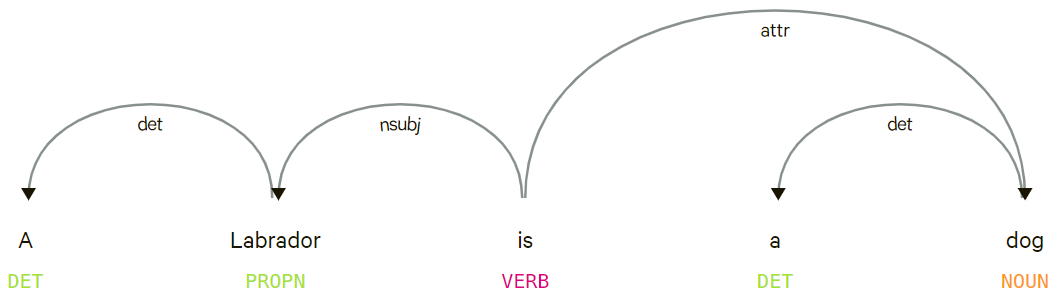
\includegraphics[width=1.\linewidth]{images/dependency_parse.png}
  \caption{Example dependency tree of a simple sentence.}%% \index{Dependency tree}}
  \label{fig:simple_dep_tree}
\end{figure}
The dependency path can be represented as a feature according to a bespoke notation.  An edge between two words can be captured with the tuple $(lemma, pos_tag, dependency_label, direction)$ and the link between two related words expressed as a list of edges.  The link between the hyponym \textit{Labrador} and its hypernym \textit{dog} would be expressed as the sequence:
\[(Labrador, PROPN, NSUB, <), (be, VERB, ROOT, -),(dog, NOUN, ATTR, >)\]

This particular notation is used in \citep{shwartz2016path} which we found more intuitive than the older convention used in \citep{Snow2004}.  To avoid longer, potentially less precise paths, a limit on the links between nouns can be imposed.  \citep{Snow2004} opted for the shortest path consisting of a maximum of four links between any two nouns.

To avoid extreme sparsity in the path vector model, \citeauthor{Snow2004} harvested dependency paths that held for at least five different word pairs from a corpus of 6 million news article sentences \citep{Snow2004}.  Doing so they generated 69,592 distinct dependency path features.  The corpus was also used to extract training and evaluation data.  As \citeauthor{wu2012probase} did later on in \citep{wu2012probase}, \citeauthor{Snow2004} extracted hyponym-hypernym word-pairs from each sentence in their corpus.  Invoking WordNet \citep{Miller1995} as lexical resource, they split the set of pairs into known hypernymy and random words.  To consider a word-pair, both of its constituent words had to be first detected in WordNet.  An ordered word-pair $(x, y)$ would be added to the known hypernym set, if $y$ is found to be an ancestor of $x$.  Words that were not hierarchically related were consigned to the random word list.  The ratio of known hypernyms to random words was 1:50.    

The dataset was used to evaluate the quality of the mined dependency paths.  This was done by applying a simple binary classifier to each path, and predicting hypernymy if a word-pair was connected by a dependency path at least once.  This exercise supplied quantitative support for the efficacy of Hearst’s manually derived patterns, all of which were found to be highly-predictive of hypernymy.  A further four patterns were also found to be high-performing:
\begin{itemize}
    \item $Y$ like $X$;
    \item $Y$ called $X$;
    \item $X$ is a $Y$;
    \item $X$, a $Y$;
\end{itemize}

\subsection{Leveraging Classifiers to Predict Hypernymy}
Intuitively, pattern occurrence frequency should be positively correlated to hypernym detection success.  \citeauthor{Snow2004} create two \ac{VSM}s.  One is a 69,592 dimensional matrix, where each dimension represents a particular dependency path and its value is the total number of times that dependency path connected an input word-pair.  They also create a bucketed, binary vector model where each dependency path corresponds to a 14-dimension “one-hot” encoded binary vector with each dimension capturing the number of pattern occurrences on an exponential scale from 1 (single occurrence) to 8192.  Thus, every word-pair is encoded as a 974,277-dimensional, sparse vector \citep{Snow2004}.  Using the same training set employed to quantify dependency path effectiveness, they train two logistic regression classifiers using each feature vector space respectively.  A significant improvement was observed compared to a simple Hearst pattern-only baseline, which classifies hypernymy if the presence of one or more Hearst patterns is found binding the input word-pair.  Their logistic regression model trained on the bucketed, “one-hot” vectors yields a 0.3480 F1 score, a 132\% improvement over the baseline \citep{Snow2004}. 
\citeauthor{ritter2009anyway}, on the other hand, advocate analysing the word form of the pattern-matched words, prior to proposing them as viable hypernym candidates \citep{ritter2009anyway}.  In particular, words detected in the plural-form by a POS-tagger are more likely to be precise hypernyms when found in certain in patterns \citep{ritter2009anyway}.  They also examine the importance of pattern occurrence frequency in their experiments, focusing on the standard Hearst patterns.  The ambiguity of the English language makes it such that high-frequency patterns alone cannot always guarantee correct hypernyms.  The authors furnish negative hypernymy examples, despite the matching highly-occurring patterns \citep{ritter2009anyway}:
\begin{itemize}
    \item \say{…all around the world including Australia, …} $\Rightarrow$ $hypernym(Australia, world)$
    \item \say{…information about this hotel such as rates, …} $\Rightarrow$ $hypernym(rates, hotel)$
    \item \say{My dog is a bloodhound} $\Rightarrow$ $hypernym(dog, bloodhound)$
\end{itemize}

They distinguish between “left” and “right” patterns where the hyponym $X$ features to the left or right of the hypernym $Y$ in a sentence.  The first two negative examples above are instances of “right” patterns and the last an incorrect instance of a “left” pattern.  \citeauthor{ritter2009anyway} engineer a set of frequency-related features for a given a word-pair.  In addition to total distinct pattern matches, they include features that capture “left” and “right” pattern matches; the total number of times that the hyponym is related to the hypernym via the lemma \textit{be}; the percentage of matches where the hyponym is preceded by an article, determiner or quantifier; the frequency rank of the hypernym with respect to the hyponym in the pair \citep{ritter2009anyway}.   

The word-pair dataset is extracted using \textsc{TextRunner} \citep{banko2007open}, applied on a 117 million web page corpus, which is then validated manually.  A test data-set consisting of 953 pairs is set aside and is split into common concepts (370 pairs) and named entities (583 pairs).  The pattern frequency vector is fed into \textsc{HypernymFinder$_{SVM}$}, a \ac{SVM} classifier \citep{platt1999probabilistic} designed to improve on an earlier na\"ive rules-based classifier that excluded hypernymy in word-pairs that did not match both left and right Hearts patterns.  An \ac{SVM} classifier splits the vector space by estimating hyperplanes which maximise the distance margin between them and the closest training-set samples.    
Unlike \citeauthor{Snow2004} who used WordNet as an evaluation and comparison tool \citep{Snow2004}, \citeauthor{ritter2009anyway} merge WordNet with \textsc{HypernymFinder$_{SVM}$} to create a hybrid classifier.  
Moreover, they opt for a hypernym discovery setup, foreshadowing the SemEval Task 2018 task 9 shared task \citep{camacho2018semeval}.  They retrofit the precision and recall metrics to measure respectively the percentage of overall correct hypermys and the percentage of terms for which one correct hypernym was proposed \citep{ritter2009anyway}.  

WordNet can return high-quality hypernyms but suffers from low coverage, especially with regards to named entities.  Each test candidate was first looked up in WordNet in which 17\% and 64\% of named entities and common nouns respectively were found.  Given some bounded vocabulary (details of which are elusive in their paper), the hybrid classifier outputs the five words it considers most likely to be hypernyms of the test words missing in WordNet.  In this manner, \citeauthor{ritter2009anyway} boosted the WordNet baseline for named entities and, to a lesser extent, common nouns.  Recall/precision increased from 0.17/1.0 to 0.32/0.9 and from 0.64/1.0 to 0.7/0.9 for named entities and common nouns respectively \citep{ritter2009anyway}.  Precision suffers with increased recall since the classifier’s output cannot be of the gold-standard level maintained in WordNet.

\subsection{Identifying Co-hyponyms to Increase Recall}
\citep{Snow2004} and \citep{ritter2009anyway} both acknowledge the limitation of Hearst patterns \citep{hearst1992automatic}.  Most hypernyms simply do not feature in the same sentence with their hyponyms \citep{Snow2004, ritter2009anyway}.  They hypothesise about extending the confines of the sentence for an “orphan” hyponym (i.e. no companion hypernym was found for it in a sentence) by finding co-hyponyms with known hypernyms.  If $(x_i, x_j)$ are two coordinate nouns and $hypernym(x_i, NA)$, $hypernym(x_j, y)$ then we can deduce $hypernym(x_i, y)$.

\citeauthor{Snow2004} experiment with various techniques including: building a distributional similarity vector space model; resorting to WordNet to find co-hyponyms for supported terms; and using high frequency conjunction dependency patterns.  Using the distributional similarity vector space the words can be scored for co-hyponym similarity using the symmetric cosine measure.  A linear combination of the probabilities calculated by the hypernym-only classifier and coordinate classifier increased the $F1$ score by 20\% compared to a hypernym-only classifier on a hand-labelled dataset ($F1$ of 0.3268 and 0.2714 respectively) \citep{Snow2004}.

On the other hand, \citeauthor{ritter2009anyway} were inspired by \textsc{Realm} \citep{downey2007sparse}, which uses \ac{HMM}s to perform type checking in an Information Extraction system, especially if the term in question is sparsely represented in vector space.  In \ac{HMM}s, a hidden stochastic process can only be glimpsed at through another stochastic process that produces a sequence of observations.  No information is known about the model's state but we can assume that there exists some model that can generate the data we're able to observe \citep{rabiner1989tutorial}.  For instance, \textit{Pickerington, Ohio} and \textit{Chicago, Illinois} are both cities but the former will be mentioned much less frequently in a balanced corpus.  Using traditional distributional similarity measures, it is unlikely that \textit{Pickerington} and \textit{Chicago} will be deemed similar since the contexts in which they appear are different.  However given an \ac{HMM} with $n$ hidden states that models the corpus, it is possible that $., Ohio$ and $., Illinois$ were generated by the same hidden states since both terms represent US States \citep{downey2007sparse} in \citep{ritter2009anyway}.

\citeauthor{ritter2009anyway} applied the same concept to finding terms similar to a given hyponym.  To do so, a word is represented by the distribution of the hidden states’ probability of the term being generated by the \ac{HMM} model.  Thus, given an \ac{HMM} model with $n$ states, an $n$-dimensional vector representation is returned.  Similar words to a given term were found by applying a similarity metric on the \ac{HMM}-based feature vector.  The final incarnation of the authors' hypernym finder, is a linear combination of the probability calculated by the \textsc{HypernymFinder$_{SVM}$} classifier and the probability that a given term $x$ has a coordinate word which is a hyponym of the candidate hypernym $y$. Since word similarity alone is tenuous evidence for such words sharing a hypernym, the \ac{HMM} classifier predicts hypernymy in a $(x, y)$ word-pair only if $x'$ exceeds a similarity threshold with $x$, and $x'$ is hyponym of $y$ \citep{ritter2009anyway}.

\subsection{Encoding Dependency Paths with an LSTM} \label{HypeNet}
We have seen that using dependency paths as features can lead to a highly-dimensional vector space.  In one study we have examined, almost 70,000 distinct dependency paths were extracted from a corpus.  Vectors will be sparse since a particular word-pair will only activate a small number of dependency paths.  To improve dependency path representation, \citeauthor{shwartz2016path} trained a \ac{LSTM} \citep{hochreiter1997long} encoder to learn path vectors that are optimised towards detecting hypernymy \citep{shwartz2016path}.  The path vectors are fed into a classifier which predicts whether the dependency pattern feature captures the hypernymy relationship in a given word-pair.  The model is referred to as \textsc{HypeNET} \citep{shwartz2016path}.

The LSTM belong to a family of neural models known as \ac{RNN}s.  Contrary to regular densely-connected networks which require an entire sequence to be presented at once, \ac{RNN}s can be fed the input, one time-step at a time \citep{chollet2017deep}.  A limitation of \ac{RNN}s is their difficulty to recognise signals that come from distant points in a past sequence which does not make them the ideal choice to learn long-term dependencies.  The \ac{LSTM} overcomes this problem because it is a type of recurrent neural network with the ability to learn long-term dependencies.  By having access to the previous time-steps, it is able to build temporal patterns.  Through the use of a special gate composed of a dot product operator and activation function, it can selectively “forget” irrelevant signals whilst retaining information that is more important at the current time-step \citep{chollet2017deep}.  

The motivation behind using the \ac{LSTM} approach is to generalise the lexical-semantic relation between terms that holds in a multitude of contexts.  Prior to feeding them to the \ac{LSTM}, each word-pair is represented by a sequence of dependency paths in which the words co-occur in the corpus.  To be considered, a word-pair needs to co-occur in the corpus and be represented by at least two unique dependency paths.  The path is represented by a list of edge vectors with each edge made up of the concatenation of the embeddings of the lemma, \ac{POS} tag, dependency label and direction.  The dimensionality of the embeddings vary: \citeauthor{shwartz2016path} use 50, 4, 5, and 1 dimension for each respective component \citep{shwartz2016path} although this is not set in stone.  Hyper-parameter tuning on a validation set can help determine the best network configuration.  The \ac{LSTM} should learn which dependency path sequences are predictive of hypernymy while conveniently forgetting those which have no consequence on the semantic relationship \citep{shwartz2016path}.

The weighted-average of the encoded dependency path vectors is computed prior to feeding it to a softmax classifier, trained to minimise cross entropy loss.  The softmax classifier assigns a probability for both the hypernymy and non-hypernymy target labels, which sum up to 1.

\citeauthor{shwartz2016path} compare their novel approach to \citeauthor{Snow2004}'s model \citep{Snow2004} we discussed in section \ref{Learning Patterns Automatically}. The authors train a logistic regression classifier on the 100,000 most information paths chosen using chi-squared feature selection.  On a random data split, the sparse model returns a precision of 0.843 compared to \textsc{HypeNET}’s 0.811 but the latter scores 0.716 recall, a 58\% improvement over \citeauthor{Snow2004}'s model.    

\section{Distributional Model Overview}
%% Need to find out how to type-set Maltese unicode characters
\say{Ghidli ma’ min taghmilha, u nghidlek x’int} is a Maltese expression which means that the company a person keeps says a lot about that person.  The linguist J.M. Firth (1957) cast a similar sentiment to words, saying that a word’s neighbours can divulge much about that word.  This dictum is framed by the Distributional Hypothesis \citep{harris1954distributional} which states that words with similar meaning occur in similar contexts.  

The Distributional Hypothesis is encapsulated in a \ac{VSM} (also referred to as distributional model), a matrix-type data structure which, at its simplest, captures the occurrences of \textit{row} events in \textit{column} contexts. The matrix’s structure in terms of what the rows and columns represent is a design decision and depends on the statistical semantic hypothesis the matrix is supposed to model.  We will briefly discuss the word-context and pair-pattern matrices, the two main types featured in the hypernymy discovery literature.  We also mention the term-document matrix, which we did not encounter in the literature review but which preceded the other two data structures and influenced their development.  The term-context feature is found at the intersection of row and column.  Features can either be expressed as raw frequencies (positive integers including 0) or can be mapped by a weighting function.  In the latter case the frequency value will be a real number.

The objective of a vector space model \ac{VSM} is to convert discrete word symbols into points in higher-dimensional space \citep{turney2010frequency}.  The word symbol does not convey any meaning through its surface form; however, by projecting each word to a multi-dimensional vector, points that are close according to some distance metric will exhibit some form of semantic relatedness.  Conversely, words corresponding to points that are far apart will tend to be weakly related or entirely unrelated \citep{turney2010frequency}.

We will discuss the matrix types in the following section.  We shall borrow the mathematical notation used in \citep{turney2010frequency} as follows:
\begin{itemize}
    \item $\textbf{X}$ will be our matrix which will be made up of $m$ rows and $n$ columns;
    \item $\textbf{X} \in \mathbb{N}^{m \times n}$ if the frequency is unweighted or $\textbf{X} \in \mathbb{R}^{m \times n}$ if we are adopting a frequency weighting mechanism;
    \item $\textbf{x}_{i:}$ will be a row-vector of $n$ elements representing a word $w_i$ in a vocabulary of terms, extracted from a corpus;
    \item $\textbf{x}_{:j}$ will be a column-vector of $m$ elements representing a document, context or pattern depending on the matrix type;
    \item $x_{ij}$ is a scalar value and measures the association between target word $w_i$ and context/pattern/document $c_j$
\end{itemize}    

Most of the elements of $\textbf{X}$ will be set to zero since a word cannot appear in all contexts and each context will correspond to a small percentage of the entire vocabulary.  Such a matrix is referred to as a sparse matrix, which contrasts with a dense matrix which has non-zero values in most of its elements.

\subsection{Mapping Vector Space Models to Semantic Hypotheses}
Word patterns can be statistically examined to understand how humans attribute meaning to the words \citep{turney2010frequency}.  Four main hypotheses were developed, supported by a corresponding mathematical matrix structure that allows each hypothesis to be explored empirically.

\subsubsection{Bag of Words}
According to the bag of words hypothesis \citep{salton1975vector}, we can represent a document in terms of the frequency distribution of the words that compose it.  The term-document matrix is the ideal structure to model this hypothesis.  X will be composed of a vocabulary of m words, extracted from n documents where each row $\textbf{x}_{i:}$ vector is a term word and each column vector $\textbf{x}_{:j}$ is a document.  Thus, the document is represented as a bag of words vector, where each dimension contains the frequency of a word $w_i$ in the document.  In the bag of words model, several aspects of language use are lost, including sequential word ordering, and syntactic links between the words.  Indeed the entirety of the document structure is absent since we cannot tell how the words were strung together in sentences, paragraphs and sections.    Despite these misgivings, the bag of words technique can effectively capture similarity between documents on the basis of word distribution alone \citep{turney2010frequency}.  This result is supported by the intuition that the domain or topic of a document influences the choice of the words used to compose the document \citep{turney2010frequency}.

\subsubsection{Word-context}
The term-document matrix may be an effective tool to measure document similarity or retrieve the most relevant documents to a given query.  However, a document is far too wide to make an ideal context if we are interested in word similarity.  The distribution hypothesis is better served by a word-context matrix.  \citep{lund1996producing} in \citep{turney2010frequency} proposed a window-based context which only considers a number of words before and after a target word.  The $k$ surrounding words of target word $w$ are: $w-k, \ldots, w-1, w+1, \ldots, w+k $.  

The typical context window size is fairly small, consisting of two to five words \citep{roller2014inclusive, santus2014chasing, shwartz2017siege}.  However, wider context windows are also acceptable.  For instance, in \citep{roller2014inclusive}, one of the context windows spanned an entire corpus sentence.

The context windows can be optionally decorated with their direction with respect to a target word \citep{shwartz2017siege}.  In the sentence \textit{The quick brown fox jumped over the lazy dog}, the directional context of the target word $fox$ is $(quick^-, brown^-, jumped^+, over^+)$. In a non-directional window, the left and right context words are indistinguishable.   

Contexts are not necessarily limited to adjacent words; \citep{lin1998information} in \citep{turney2010frequency} and \citep{levy2014dependency} employed dependency-based contexts.  To build their experimental distributional semantic spaces, \citep{shwartz2017siege} considers both parent-daughter and parent-sister neighbours in a dependency tree.

\subsubsection{Pair-pattern}
The term, represented in the matrix row, is no longer a single word but a word-pair and the matrix column feature becomes a doubly-linked pattern which ties the term word-pair together.  We have seen a pair-pattern matrix in action in \citep{Snow2004}.  The term pair is a tuple containing a hyponym and a candidate hypernym.  Tuples can be positive or negative pairs depending on whether the candidate word is an actual hypernym.  The matrix column feature was a dependency path which linked the two words together by the concatenation of edge links in the parse tree and the feature value was the frequency a word-pair matched that particular pattern.

\citep{lin2001discovery} quoted in \citep{turney2010frequency}, propose the extended distributional hypothesis which states that patterns fitting similar pairs tend to have the same semantics.  Conversely, the latent relation hypothesis states that word pairs captured by similar patterns tend to be bound by a similar semantic relation \citep{turney2010frequency}.  \citep{Snow2004} opted for a supervised approach and utilised various classifiers to learn which paths were mostly indicative of hypernymy.  The path feature set they induced included any path that linked at least five distinct nouns pairs extracted from each sentence in the corpus.  

A variant of the pair-pattern matrix is \textbf{TypeDM} \citep{roller2014inclusive}, where a matrix row represents a term word and the context column is a pair consisting of a context word and a syntagmatic relationship that ties the two words together.

\subsection{Feature Weighting}
At its most elemental, each matrix type quantifies the association between a context and a term by counting the occurrences of the term in a particular context \citep{turney2010frequency}, \citep{shwartz2017siege}.  Often, the raw frequencies are adjusted to compensate for the fact that some words convey little information despite their high recurrence in a corpus.  In the bag of words model, the raw frequencies are transformed using the \textbf{\ac{tf-idf}} function family \citep{turney2010frequency}.  This compels a term to score a high weight if its presence in a document is proportional to its scarcity in other documents.

An alternative to \ac{tf-idf} used to weight features in a word-context matrix is \ac{PMI}:
\[PMI(w_i, c_j) = log \Bigg( \frac{p(w_i, c_j)}{p(w_i)p(c_j)} \Bigg) \]
\ac{PMI} measures the log ratio of the joint probability of a word $w_i$ in a context $c_j$ and the product of the marginal probabilities of $w_i$ and $c_j$ \citep{church1990word} in \citep{turney2010frequency, shwartz2017siege}.

If there is an interesting relationship between $w_i$ and $c_j$, then the conditional probability of $w_i$ given $c_j$ is greater than the joint probability of $w_i$ and $c_j$ given that the two are mutually exclusive.  When that is the case, \ac{PMI} returns a positive value.  On the other hand, if $w_i$ and $c_j$ are independent, \ac{PMI} returns a zero value.  If the presence of a particular context decreases the probability of a word co-occurring, then $p(w_i, c_j)$ is smaller than $p(w_i)p(w_j)$ and a negative \ac{PMI} is returned.

A variant of \ac{PMI} is \ac{PPMI} which enforces every matrix element to be positive or zero if a word does not occur in a particular context.  \ac{PPMI} is biased towards rare events \citep{turney2010frequency} but this can be neutralised by the application of \ac{PLMI} which is returned when \ac{PPMI} is multiplied by the co-occurrence frequency of $w_i$ and $c_j$ \citep{evert2008corpora} in \citep{shwartz2017siege}.

\subsection{Building a Vector Space Model}
A pre-processing pipeline is applied to a corpus before it can be transformed into a matrix-based mathematical model.  The pipeline includes tokenisation, normalisation and, optionally, annotation steps \citep{turney2010frequency}.

At first glance, tokenisation of an English corpus may seem like a trivial task since words are conveniently separated by spaces and sentences divided by the full-stop punctuation mark.  A tokeniser must, however, contend with specificities such as hyphenated words, abbreviations, diverse use of punctuation (ex. \textit{can’t}, \textit{isn’t}, etc.) and multi-word phrases that should be treated atomically (ex. \textit{catch fire}, \textit{vice president}, \textit{Daniel Day-Lewis}) .  Pictogram-based languages such as Chinese and Japanese are harder to deal with since words are not separated by spaces to begin with \citep{turney2010frequency}.

Words expressed with different lexicalisations can sometimes have the same meaning.  A chief example is the capitalisation of a word at the beginning of a sentence which does not change the meaning of the word. Normalisation smoothens surface form variation by lower casing and stemming words. Stemming reduces a word to its most generic form which may not be an actual word.  Highly specific word forms can harm recall which is thus augmented by normalisation but only at the expense of precision \citep{kraaij1996viewing} in \citep{turney2010frequency}.

Annotation increases the specificity of a word by decorating it with descriptors such as the part-of-speech tag, word sense tag, and dependency parse labels.  Word sense disambiguation is particularly relevant in the field of hypernymy detection and discovery since disparate meaning is often attributed to identical word forms.  The hypernym of \textit{bank} can either be \textit{incline} or \textit{financial institution} depending on its word sense.  The attachment of more information to a word is expected to increase precision while punishing recall \citep{turney2010frequency}.

We briefly mentioned all the components needed to build a \ac{VSM} from pre-processing to feature weighting.  To find the degree to which $y$ is a hypernym of $x$ in word-pair $(x, y)$, a metric is applied to the vector representation of $x$ and $y$.  The metrics are collectively referred to as unsupervised methods since they are applied without the need of training data.  In the following section we explore unsupervised methods within selected literature.

\section{Unsupervised Methods}
\subsection{Metric Overview}
Unsupervised methods consists of metrics grouped into four categories, each representative of a hypernymy inflected semantic hypothesis.  \citeauthor{shwartz2017siege} furnish us with an exhaustive survey of metrics across all categories which are listed below.  In all descriptions, $\textbf{x}$ and $\textbf{y}$ represent the term word (hyponym) and candidate hypernym feature vector respectively.  A summary of unsupervised measures which can be used to estimate hypernymy simalarity can be seen in Table~\ref{tab:unsupervised_measures}.

%% Table summarising the measures and grouping them by hypothesis needs to come here
\renewcommand{\arraystretch}{1.2} 
\begin{table*}\centering
    \begin{tabular}{@{}ll@{}} \toprule
    \textbf{Metric}              & \textbf{Source} \\ 
    \cmidrule{1-2}
    \multicolumn{2}{c}{Similarity Measures} \\ \cmidrule(lr){1-2}
    $Cosine Similarity$   & \citep{salton1975vector} \\
    $Lin Similarity$      & \citep{lin1998information} \\
    $APSyn$               & \citep{santus2016unsupervised} \\
    \cmidrule{1-2}
    \multicolumn{2}{c}{Inclusional Measures} \\ \cmidrule(lr){1-2}
    $Weeds Precision$     & \citep{weeds2003general} \\
    $cosWeeds$            & \citep{lenci2012identifying} \\ 
    $ClarkeDE$            & \citep{clarke2009context} \\
    $balAPinc$            & \citep{kotlerman2010directional} \\
    $invCL$               & \citep{lenci2012identifying} \\
    \cmidrule{1-2}
    \multicolumn{2}{c}{Informativeness Measures} \\ \cmidrule(lr){1-2}
    $SLQS$                & \citep{santus2014chasing} \\
    $SLQS_{Sub}$            & \citep{shwartz2017siege} \\
    $SLQS_{Row}$            & \citep{shwartz2017siege} \\
    \cmidrule{1-2}
    \multicolumn{2}{c}{Reversed Inclusional Measures} \\ \cmidrule(lr){1-2}
    $Reversed Weeds$      & \citep{shwartz2017siege} \\
    $Reversed ClarkeDE$   & \citep{shwartz2017siege} \\
    \bottomrule
    \end{tabular}
    \caption{Unsupervised Hypernymy Similarity Measures.}\label{tab:unsupervised_measures}
\end{table*}


\subsubsection{Similarity Measures}
Following the distributional hypothesis \citep{harris1954distributional}, similarity measures focus on the symmetric similarities between the hyponym and hypernym.  Cosine similarity is the inner product of the unit-normalised vectors $\textbf{x}$ and $\textbf{y}$, thus placing the onus of similarity on the angle between the vectors.   The cosine metric measures word similarity by the angle between the vectors $\textbf{x}$ and $\textbf{y}$ where acute angles indicate higher similarity.  The Lin measure is the ratio between common contexts and separate contexts of $\textbf{x}$ and $\textbf{y}$.  A high-level explanation of $APSyn$ can be found in \citep{shwartz2017siege} and more details in \citep{santus2016unsupervised}.

\subsubsection{Distributional Inclusional Measures}
A common criticism of the measures based on the distribution hypothesis is that they are not able to discern among various semantic relations \citep{roller2014inclusive}.  A term word’s nearest neighbours will bear some semantic relationship to it but is not guaranteed to be its hypernym. Moreover, the distributional hypothesis fails to acknowledge the asymmetric nature of hypernymy.  Instead, this is better captured by the distributional inclusional hypothesis \citep{geffet2005distributional} which states that the main contexts of the hyponym term are absorbed in the contexts of its hypernym.  According to this hypothesis, plugging in the generic term instead of the specific term in a sentence would not warp the sentence’s meaning.  $Weeds Precision$ \citep{weeds2003general} is an example of an asymmetric metric that computes the weighted inclusion of the contexts of $\textbf{x}$ within the contexts of $textbf{y}$.  Details of the other measures may be found in their respective papers.

$invCL$ \citep{lenci2012identifying} is another example of an inclusional metric which is calculated as the geometric mean of the degree of inclusion of the hyponym’s contexts in the hypernym’s contexts  and the non-inclusion of the hypernym’s contexts into the hyponym’s contexts.


\subsubsection{Distributional Informativeness Measures}
\citeauthor{santus2014chasing} debated the validity of the distributional inclusional hypothesis.  They argue that the distinction between a hyponym and a hypernym lies in the generality of their contexts.  By virtue of their abstract qualities, hypernyms occur in broad contexts.  Their hyponyms, on the other hand, are specific and thus more likely to feature in explicit contexts.  For instance, an animal has general properties of locomotion, feeding and reproduction but only the echidna and platypus will feature in the context of egg-laying mammals.

The distributional informativeness hypothesis is derived from this principal.  $SLQS$ \citep{santus2014chasing} employs entropy to quantify informativeness.  Lower entropy values imply less uncertainty about the outcome of an event.  Hence, the more general the contexts, the lower the probability we can guess the “topic” of reference and the higher the entropy value.  $SLQS$ calculates the reciprocal difference of the median entropy of the top $N$ contexts of hyponym and hypernym vectors.  $SLQS$ is also an asymmetric measure and if $SLQS(x, y)$ yields a positive value, then $\textbf{y}$ is found to be more general than $\textbf{x}$ which is an indicator of hypernymy.  Three further variants of $SLQS$ were first proposed in \citep{shwartz2017siege}.  $SLQS_{Sub}$ is a weakly symmetric version of $SLQS$ evaluated by subtracting the median entropy of a hyponym's top $N$ contexts from the median entropy of its hypernym's top $N$ contexts.  $SLQS_{Row}$ exploits the fact that the context and target word entropies are not highly correlated, thus repositioning $SLQS$ in terms of target word entropy \citep{shwartz2017siege}.  Finally, $SLQS_{Row, Sub}$ uses the same subtraction expression as $SLQS_{Sub}$ on $SLQS_{Row}$.

\subsubsection{Reversed Inclusional Measures}
The distributional inclusional hypothesis is directly challenged by the reversed inclusional measures.  The basis of these measures is the hypernym cannot always replace the hyponym in its contexts due to the high specificity of the latter.  \textit{The mammal climbed into the car} would not be a reasonable alternative for \textit{the man climbed into car} despite the fact that a man is a mammal.  \citep{shwartz2017siege} propose a simple variant of Weeds Precision and ClarkeDE to model this property, consisting of switching the original function parameters around.  Thus $WeedsPrec(x,y)$ becomes $ReversedWeedsPrec(y, x)$ and the same principle applies to ClarkeDE.

\subsection{Application of Unsupervised Metrics in Selected Literature} \label{shwartz_unsupervised}
In \citep{santus2014chasing},  a 2.7-billion word corpus was constructed by concatenating the ukWaC \citep{ferraresi2007building} and WaCkypedia corpora in English \citep{baroni2009wacky}.  Word context was provided by a two-word window on either side of the target word and \ac{LMI} was used to weight the features.  The BLESS dataset \citep{Baroni2011} was recruited as an evaluation dataset.  Besides providing hypernyms for 200 English concepts, BLESS also features several negative examples of hypernymy which include other semantic relations such meronym, co-hyponymy and randomly unrelated words.

\citeauthor{santus2014chasing} pitted the distributional inclusional and informativeness hypotheses against each other over two tasks.  $WeedsPrec$ \citep{weeds2003general} represents the inclusional metric family while the informativeness hypothesis is represented by $SLQS$ \citep{santus2014chasing}.  The first tasks involves detecting hypernymy in each positive word-pair using the most frequently occurring word as a baseline.  The second, harder task consisted of discriminating hypernymy from the other semantic relations.

\begin{table*}\centering
    \begin{tabular}{@{}lrrrr@{}} \toprule
    \textbf{Metric}  & \textbf{Hypernymy} & \textbf{Co-hyponymy} & \textbf{Meronymy} & \textbf{Unrelated} \\
    \cmidrule{1-5}
    \textit{Baseline}   & $0.40$ & $0.51$ & $0.38$ & $0.17$ \\
    \textit{Cosine}   & $0.48$ & $0.46$ & $0.31$ & $0.21$ \\
    \textit{WeedsPrec}   & $0.50$ & $0.35$ & $0.39$ & $0.21$ \\
    \textit{SLQS $\times$ Cosine}   & $\textbf{0.59}$ & $\textbf{0.27}$ & $\textbf{0.35}$ & $\textbf{0.24}$ \\
    \bottomrule
    \end{tabular}
    \caption{Average precision of two unsupervised metrics when discriminating semantic relations.}\label{tab:santus_comparison}
\end{table*}

$WeedsPrec$ does not beat the baseline in the first task, scoring a precision of $0.6304$ (compared to a $0.6609$ baseline) while $SLQS$ does better, yielding a precision score of $0.87$.  Distributional similarity is leveraged in the second task by assuming that a hypernym observes two rules: the hyponym must be distributionally similar to the hypernym; the hypernym must be more general than the hyponym.  To merge the two, the product of cosine similarity and positive $SLQS$ is computed.  Precision is replaced by \ac{AP} as evaluation metric where \ac{AP} evaluates the ranking of the predicted hypernymy word-pairs against false positives pertaining to other relations.  The results are reproduced in Table~\ref{tab:santus_comparison} from \citet{santus2014chasing}.

$SLQS$ is less likely to confuse co-hyponymy for hypernymy than $WeedsPrec$ which suggests that in general the co-hyponym in the candidate word slot ($y$) is as specific as the query word ($x$).  The scores reflect the average precision over all 200 concepts in the BLESS dataset ($AP@all$).

In \citep{shwartz2017siege}, the authors undertake a more ambitious study of unsupervised metrics over four commonly-used datasets: BLESS \citep{Baroni2011}; EVALution \citep{santus2015evalution}; Lenci/Benotto \citep{benotto2015distributional}; and Weeds \citep{weeds2014learning}.  Each dataset features positive hypernymy examples and negative examples consisting of words that are related together via some other semantic relationship such as meronymy, synonymy, co-hyponymy or randomly unrelated.  The study tests each metric’s ability at distinguishing hypernymy from the other relations.  Furthermore, experiments were also carried out to measure the metric’s performance at detecting hypernymy among specific relations in isolation. 

\begin{table*}\centering
    \begin{tabular}{@{}cccc@{}} \toprule
    \textbf{Context Type} & \multicolumn{2}{c}{\textbf{Context Parameters}} & \textbf{Feature Weighting} \\ \cmidrule{1-4}
    \multirow{6}{*}{Window} & 
    \multirow{3}{*}{Directional} &
    \multirow{3}{*}{$win2d$ or $win5d$} & Raw Freq \\
    & & & PPMI \\
    & & & LMI \\ 
    \cmidrule{2-4}
    & \multirow{3}{*}{Non-Directional} &
      \multirow{3}{*}{$win2$ or $win5$} & Raw Freq \\
    & & & PPMI \\
    & & & LMI \\ 
    \cmidrule{1-4}
    \multirow{3}{*}{Dependency} & 
    \multirow{3}{*}{-} &
    \multirow{3}{*}{$dep$ or $joint$} & Raw Freq \\
    & & & PPMI \\
    & & & LMI \\
    \bottomrule
    \end{tabular}
    \caption{Vector Space Model combinations used in \citep{shwartz2017siege}.}\label{tab:siege_vector_spaces}
\end{table*}

Following \citep{santus2014chasing}, \citeauthor{shwartz2017siege} make use of the same concatenated corpus but in contrast to \citeauthor{santus2014chasing}, lemmatised it and annotated it with part-of-speech tags and dependency labels.  The \ac{VSM}’s vocabulary was limited by only considering nouns, verbs and adjectives that featured 100 times or more in the corpus.  Several \acl{VSM}s were constructed in an attempt to determine which particular combination, in tandem with an unsupervised metric, works best at identifying hypernymy among several relata.  

Table~\ref{tab:siege_vector_spaces} illustrates the \ac{VSM} variants tested.  The authors tested window and dependency-based contexts, with the association between the words and their contexts weighted by raw frequency, \ac{PPMI}, and \ac{PLMI} for a total of 18 matrix combinations. $win2$ and $win5$ represent a two and five word non-directional context window respectively, whereas the $d$ suffix denotes a directional context.  The dependency-based contexts are denoted by $dep$ and $joint$, where the former represents parent-daughter context and the latter captures parent-sister pairs in the dependency tree.

\begin{table*}\centering
    \begin{tabular}{@{}lccccr@{}} \toprule
    \textbf{Dataset} & \shortstack{\textbf{Hyper vs.} \\ \textbf{Relation} } & \textbf{Measure} & \shortstack{\textbf{Context} \\ \textbf{Type} } & \shortstack{\textbf{Feature} \\ \textbf{Weighting}} & \textbf{AP@100} \\ \cmidrule{1-6}
    \multirow{5}{*}{EVALution} & 
    All Relations & $invCL$ & joint & freq & 0.661 \\
    & Meronym & $APSyn$ & joint & freq & 0.883 \\
    & Attribute & $APSyn$ & joint & freq & 0.880 \\
    & Antonym & $SLQS_{Row}$ & joint & freq & 0.740 \\
    & Synonym & $SLQS_{Row}$ & joint & freq & 0.830 \\
    \cmidrule{1-6}
    \multirow{5}{*}{BLESS} & 
    All Relations & $invCL$ & win5 & freq & 0.540 \\
    & Meronym & $SLQS_{Sub}$ & win5d & freq & 1.000 \\
    & Coordinate & $SLQS_{Sub}$ & joint & freq & 0.995 \\
    & Attribute & $SLQS_{Sub}$ & dep & PLMI & 1.000 \\
    & Event & $APSyn$ & dep & freq & 1.000 \\
    \cmidrule{1-6}
    \multirow{3}{*}{Lenci/Benotto} & 
    All Relations & $APSyn$ & joint & freq & 0.617 \\
    & Antonym & $APSyn$ & dep & freq & 0.861 \\
    & Synonym & $SLQS_{Row, Sub}$ & joint & PPMI & 0.948 \\
    \cmidrule{1-6}
    \multirow{2}{*}{Weeds} & 
    All Relations & $ClarkeDE$ & win5d & freq & 0.911 \\
    & Coordinate & $ClarkeDE$ & win5d & freq & 0.911 \\
    \bottomrule
    \end{tabular}
    \caption{Subset of best unsupervised results in \citep{shwartz2017siege}.}\label{tab:siege_unsupervised_results}
\end{table*}

For each measure, context-type, feature weighting function, the word-pairs were ranked in descending order of the score achieved.  The \ac{AP} was measured in two instances: on the full list of word-pairs; and on the 100 most confidently scored pairs.  A table reflecting the best $AP@100$ results recorded in the experiments is shown in Table~\ref{tab:siege_unsupervised_results} from \citet{shwartz2017siege}.

Results suggest that there does not exist one combination of measure and semantic space that outperforms the rest across the board.  Supported by the best results, the authors speculated that syntactic contexts (dependency, joint-dependency) have higher hypernymy predictive power due to them capturing both proximity and syntactic features.  The na\"ve raw frequency feature weight acquitted itself surprisingly well considering it does not provide more information than co-occurrence of word and context.

The nature of the word-pairs in the datasets influenced the experiments’ outcome and shed some light on why some metrics fared better on some datasets than others.  $SLQS$ outputs a high score if the candidate word being tested for hypernymy is found to be more general than the query word \citep{santus2014chasing}.  It performed well (although not necessarily the best) in the hypernymy/antonymy, hypernymy/synonymy challenges where the (negative) candidate antonyms and synonyms were largely less general than the hypernyms in the set.  Conversely, the symmetric similarity measures were best suited to distinguish hypernymy from words which have few shared contexts.  For instance, the attribute words featured in BLESS are adjectives which share few contexts with the noun term word.  

Like \citep{santus2014chasing}, $SLQS$ was more effective at recognising hypernymy than inclusion-based methods, even when applied onto dependency-based context types.  However, inclusion-based methods such as $ClarkeDE$, $invCL$ and $WeedsPrec$ were superior to $SLQS$ on the Weeds dataset.  \citeauthor{shwartz2017siege} conclude that this result is due to the distribution of words in Weeds, in which every positive and negative hypernym instance features only once.  BLESS contains several repeated hypernyms which, moreover, tend to be rather general (ex. \textit{animal}, \textit{object}).  This plays to the strengths of $SLQS$ which justifies its dominance on this particular set.

\subsection{Criticism of Unsupervised Methods}
We examined empirical work which illustrated the power of unsupervised metrics, founded as they are on sound linguistic hypotheses.  Although the metrics have been used in a hypernymy detection context, they can be leveraged to discover hypernyms by finding the nearest neighbours of a hyponym vector in a particular vector space according to an asymmetric measure based on the distributional inclusional or informativeness hypothesis like the baselines created by the SemEval 2018 Task 9 organisers \citep{camacho2018semeval}.  For unsupervised methods to be effective in this regard, the score returned when considering a hypernymy word-pair must be statistically distinguishable from the score returned if the word-pair is random or linked by some other semantic relation.  Otherwise recognising hypernyms using such methods is reduced to a game of chance.  Although \citep{santus2014chasing} challenged the soundness of inclusion measures, \citep{roller2014inclusive} tested whether asymmetric metrics based on the inclusional hypothesis are able to fulfill this requirement and, unfortunately, found them initially lacking.

\citeauthor{roller2014inclusive} construct a corpus in a manner similar to \citep{santus2014chasing}, but enlarged by the inclusion of Gigaword and BNC.  The authors pre-processed the corpus by lemmatising it and annotating the part-of-speech tags, after which they filtered out words which occurred less than 500 times.  They constructed three vector spaces, two of which were based on a window context (2 words around the target word, and a full sentence respectively), and one based on a TypeDM tensor model.  The vector spaces are denoted as \textit{U+W2}, \textit{U+Sent} and \textit{TypeDM} respectively.  The features of the two window-based models were transformed by \ac{PPMI}.

\begin{figure}[ht!] 
  \centering
  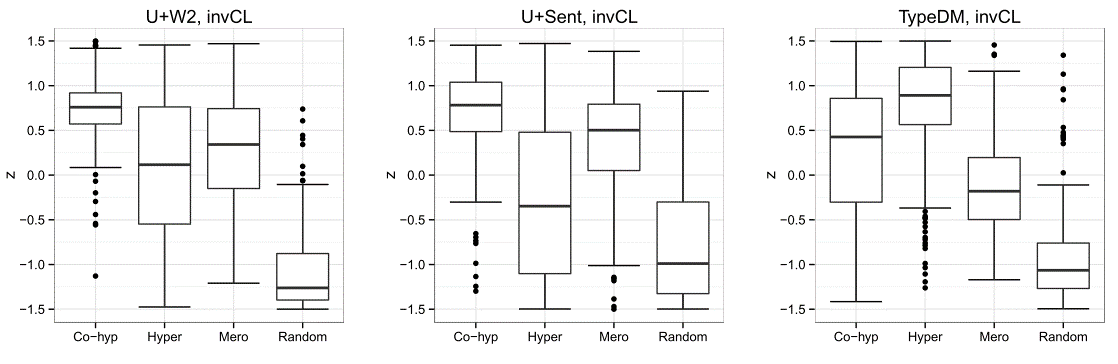
\includegraphics[width=1.\linewidth]{images/standardised_distribution_invCL.png}
  \caption{Standardised distribution of $invCL$ score in \citep{roller2014inclusive}.}
  \label{fig:standardised_invCL_boxplot}
\end{figure}

A battery of inclusional measures, including $WeedsPrec$ \citep{weeds2003general} and $invCL$ \citep{lenci2012identifying}, were used to score the word-pairs in the BLESS dataset \citep{Baroni2011} in each vector space which, as we have already seen, consists of word-pairs tied by several semantic relations.  The scores were standardised and a box-plot of the score achieved when measuring $invCL$ asymmetric similarity - chosen for the best results attained in the experiment - across relations and vector spaces is reproduced in Figure~\ref{fig:standardised_invCL_boxplot} from \citet{roller2014inclusive}.

Despite $invCL$ was the most productive metric at hypernym identification, we can see that performance is not robust across all vector space models.  The standardised $z$-score was significantly higher for hypernymy word-pairs in the \textit{TypeDM} space but was entirely deprived of predictive ability in the \textit{U+W2}  and \textit{U+Sent} \ac{VSM}s. \ac{AP} results for hypernymy against co-hyponymy, meronymy and random relation respectively, depict a similar picture.  In all vector spaces except \textit{TypeDM}, both the asymmetric measures as well as the baseline cosine symmetric measures assigned the highest ranking to co-hyponym terms by a significant margin.  In \textit{TypeDM}, $invCL$ acquires a higher mean average precision for hypernyms than for co-hyponyms but the difference is not statistically significant \citep{roller2014inclusive}.

These experiments pose a conundrum for unsupervised methods research: they have been shown to be successful in some settings but clearly miss the mark in others.  \citeauthor{roller2014inclusive} argued that the distributional inclusional hypothesis was selective and did not apply on all contexts.  However, unsupervised methods of distributional inclusion considered all contexts equally, which ultimately harms their performance \citep{roller2014inclusive}.  They propose a technique similar to \citep{Snow2004}, which leverages a supervised classifier to both learn the distributional signals most associated with a given set of hypernymy word-pairs, and interpret the trained models to understand which features are contributing to the estimated result.

\section{Supervised Methods}
High-quality, ground-truth data and associated target discrete labels (or continuous values if the task is of the regression type), distinguish supervised methods from the unsupervised measures we have reviewed so far.  In the hypernymy identification domain, supervised methods are not grounded in a linguistic hypothesis but attempt to learn the asymmetric metric from a provided training set \citep{levy2015supervised}.

Just like in the unsupervised context, the query and candidate hypernym terms are represented by vectors sourced from a vector space model.  Instead of applying distributional hypotheses, the vectors representing the words in the pair are combined by a vector operations like concatenation \citep{baroni2012entailment}, or difference \citep{roller2014inclusive}.  In the concatenation case, the hypernym vector is added to the tail of the hyponym vector to create a feature which has twice the number of dimensions as the individual word vector.  In the diff case, the hypernym vector is subtracted from the hyponym \citep{roller2014inclusive} or vice versa \citep{shwartz2017siege}.  The combined feature vectors are fed into a classifier together with the target labels.  The literature we reviewed shows a preference for the logistic regression \citep{roller2014inclusive, shwartz2017siege, levy2015supervised, yamane2016distributional, bernier2018crim} and \ac{SVM} classifiers \citep{shwartz2017siege, levy2015supervised, baroni2012entailment}.

\subsection{Classifier Background}
\subsubsection{Logistic Regression}
Despite the name, logistic regression is actually a binary classification learning algorithm that uses the properties of the logistic function $\sigma(z)=\frac{1}{1 + e^{-z}}$ that maps real valued inputs to values between $0$ and $1$.  Values in this range can be interpreted as a probability. The real value input is a linear combination of $m$ features and $m+1$ weights.  This can be expressed in the terms of the logit function: \[logit(p(y = 1 \mid x)) = z = \textbf{w}^T\textbf{x}\]

The resulting real value can be mapped to a probability using the defined logistic equation.  To learn the best weights (or coefficients) a cost function is required to minimise the error when predicting hypernymy.  This is done by minimising the logistic loss function: 
\[J(w) = \sum_{i=1}^{n}\Big[-y^{(i)}log\big(\sigma(z^{(i)})\big) - \big(1 - y^{(i)}\big) log\big(1-\sigma(z^{(i)}\big)\big)  \Big] \] 

The linear model for binary classification can be extended to the multiclass classification via the \textit{OvR} (one vs rest technique) or using multiclass settings that optimise the model for multi label classification.  Deviations from the correct prediction push the cost function towards infinity thus penalising poor predictions. 

Various gradient descent solvers can be used to minimise the cost function but some are better suited than others depending on the circumstances.  Adam \citep{kingma2014adam} is a sophisticated version of the standard \ac{SGD} solver which attempts to minimise the task’s cost function by taking tiny steps in the direction opposite to the gradient calculated from the cost function’s derivative.  Adam is distinguished from vanilla \ac{SGD} by managing an adaptive learning rate for every trainable parameter.  It is known to work well in several empirical scenarios and is used extensively in the literature we reviewed \citep{shwartz2016path, bernier2018crim, yamane2016distributional, espinosa2016supervised}.

Two problems afflict all machine learning algorithms: bias and variance.  High bias means that the model does not learn enough from the training data, under-fitting the data and does not generalise well to unseen instances.   High variance is when the model misinterprets random noise in the data as important features which do not carry over to new unseen instances.  Variance and bias in logistic regression models can be tuned with the addition of regularisation parameters that penalise extreme feature coefficients. $L2$ regularisation penalises large weights whereas $L1$ encourages sparse solutions – weight coefficients set to $0$, thus nullifying the effect of the corresponding feature on the model.  Because of this reason, $L1$ regularisation is often used as a feature selection technique.

\subsubsection{Support Vector Machines}
%% to be added

\subsection{Representative Work} 
\citeauthor{baroni2012entailment}'s work \citep{baroni2012entailment} is considered a baseline in the literature under review \citep{shwartz2017siege, shwartz2016path, camacho2017we, roller2014inclusive, levy2015supervised}.  The study focused on two tasks, but we shall ignore the second task which is related to learning quantifying determiners (ex. \textit{few} entails \textit{some}).  

In the first task, the authors wanted to capture training data for an entailment recogniser by leveraging properties of adjective-noun (AN) composite expressions, such as \textit{red car}.  Based on the fact that most ANs imply the headword noun (\textit{white cat} entails \textit{cat}), the vector equivalent of these pairs can be used to train a classifier to detect hypernymy for other nouns (\textit{cat} entails \textit{animal}).  Like hyponyms, adjective-noun phrases are more specific than the noun and hence their contexts are a subset of the context of the modified noun. 

Corpus pre-processing steps mirror what we have already described in other work.  The author uses a sentence wide word-window context and the features were transformed by \ac{PMI}.  A sparse vector space model composed of $48,000$ target word vector rows and $27,000$ context word columns.  To counter the matrix’s sparsity and improve computation efficiency, the vector was reduced to $300$ components via an \ac{SVD} transformation.  The training data set, partially generated from BLESS, included $1,246$ positive $(AN, N)$ pairs.  Negative instances were induced automatically by linking ANs with randomly-selected nouns in the dataset.  The test set, which had to be composed of (hyponym, hypernym) pairs, was culled from WordNet \citep{Miller1995}, avoiding hypernyms which are too abstract (ex. \textit{object}, \textit{entity}, etc.).  Negative instances were generated using the same method employed in the training set.  

To build the feature vector, \citeauthor{baroni2012entailment} concatenated the vector equivalent of each training pair component together.  Since the vector space was reduced to $300$ dimension, each feature was composed of a $600$-dimension vector.  The author opted for an \ac{SVM} with polynomial kernel to learn the entailment signal.  They supported their choice by noting that a non-linear \ac{SVM} extracts feature interactions automatically, which would otherwise have had to be handcrafted in order to be exploited by a linear classifier like a logistic regression model.  They trained their \ac{SVM} on the $(AN, N)$ pairs and achieved a $69.3\%$ accuracy score when they evaluated the model on the hypernymy test set.  Accuracy ascended to $88.6\%$, when they trained the \ac{SVM} directly on the hypernymy set with $10-$fold cross-validation.  The results showed that a model trained to recognise the head noun in adjective-noun pairs can be effectively transferred to the related - but different - task of distinguishing hypernyms from random words.

\citeauthor{roller2014inclusive} use vector difference to construct their features.  Inspired by the success of \citeauthor{mikolov2013distributed} at using vector subtraction to learn word analogies \citep{mikolov2013distributed}, they come up with their own vector difference variant.  They represent each word-pair by the difference of the unit-normalised vectors, combined with their square differences.  

These features are intended to capture both the dimensions that strongly predict hypernymy and the dimensions that are predictive of random words.
The authors construct a vector space with a sentence wide word-window similar to \citep{baroni2012entailment}.  The corpus used by \citep{roller2014inclusive} differs from \citep{baroni2012entailment} only by the inclusion of Gigaword in addition to BNC, ukWaC and WaCkypedia.  The resultant vector space is reduced to $300$ dimensions by \ac{SVD}, once again mirroring \citeauthor{baroni2012entailment}'s setup.  

The training data were provided by the BLESS and ENTAILMENT datasets.  Instead of splitting the datasets into training and test, they opt to measure the classifier’s ability at identifying hypernyms on all terms in the sets.  To do so, they holdout one term and train on the remaining terms.  Additionally, they carry out a lexical split whereby they ignore any word-pairs in the training set which overlaps one of the words in the test, irrespective of position.  An average accuracy score of $0.80$ and $0.82$ is achieved on BLESS and ENTAILMENT respectively, considerably beyond the most frequent class baseline of $0.46$ and $0.50$ respectively.  \citeauthor{roller2014inclusive} also train an \ac{SVM} classifier on concatenated features and experiment with a variety of vector spaces, achieving similar results.  However, the logistic regression model trained on $diff$ features beat the \ac{SVM} in every experiment attempted.  For the sake of comparison, we specifically cited the result attained on the experiment which was, in our view, most similar to \citep{baroni2012entailment}.

\subsection{"Curse of Dimensionality"}
Vector space models tend to be highly dimensional due to the large number of contexts that feature in any sizable corpus.  Training classifiers on hundreds of thousands of features results in an overly complex model that may struggle to capture the variance in the data.  Singular value decomposition is a dimension reduction technique which projects the sparse highly-dimensional matrix onto a low-dimensional, dense vector space.  To do so, it factorises a matrix $\bm{X}$ into three component matrices $\bm{U}\bm{\Sigma}\bm{V^T}$, where $\bm{U}$ represents a spatial transformation of words, $\bm{\Sigma}$ (also known as singular values) provides weights for those words and $\bm{V}$ is a spatial represenation of the contexts.  As with all dimension reduction techniques, some information is lost from the original matrix but the smaller vectors makes it more suitable for training supervised classifiers.  However, in transforming the original axes, the reduced \ac{VSM}’s dimensions become latent and no longer easily interpretable \citep{levy2015supervised}.

From a practical standpoint, the data compression that is brought about by the application of feature extraction results in a computationally more efficient model which is required to learn a fraction of the parameters it would have otherwise had to learn on the original vector space.  \ac{SVD} is used to reduce the vector space in several work we reviewed \citep{baroni2012entailment, roller2014inclusive, levy2015supervised}.  The number of \ac{SVD} components is a configurable hyper-parameter which can be tuned on a validation dataset, but the studies we examined opt for 300 to 500 dimensions.

\subsection{Lexical Memorisation}
\citeauthor{levy2015supervised} bring a dose of scientifically-grounded scepticism to the proceedings by claiming that the supervised methods we mentioned do not actually learn inferential relations but merely detect mutually independent features associated with the words in isolation.  In doing so, they showed that supervised classifiers trained on vector combinations memorise frequently-seen hypernyms and then predict hypernymy whenever the “prototypical hypernyms” turn up in a word-pair \citep{levy2015supervised}.

To prove that their hypothesis is not dependent on a particular vector space or supervised method, they built a comprehensive experimental setup which allowed them to compare various state-of-the-art approaches.  They created nine vector spaces by crossing three context types with three feature weighting functions:
\begin{itemize}
    \item Three context types:
    \begin{itemize}
        \item Directional word-window using two words on either side of the target word;
        \item Non-directional word-window considering five words on either side of the target word;
        \item Dependency context which chooses all word that are syntactically connected to the target word;
    \end{itemize}
    \item Three feature weighting functions:
    \begin{itemize}
        \item \ac{PPMI};
        \item \ac{PPMI} + dimension reduction to 500 components via \ac{SVD};
        \item Skip-gram with negative sampling which will be discussed in the word embeddings section;
    \end{itemize}
\end{itemize}
Moreover, to show that there is no bias to a particular dataset, they evaluate their models on five labelled datasets: 2 versions of \textit{BLESS} \citep{Baroni2011, baroni2012entailment}; \textit{Kotlerman} \citep{kotlerman2010directional}; \textit{Turney and Mohammad} \citep{turney2015experiments}; and \textit{Levy} \citep{levy2014focused}.  Each dataset was created to capture different semantic relations other than hypernyms including entailment nuances such as causality.  Interestingly, the \textit{Weeds} dataset \citep{weeds2014learning} was eschewed, probably because the dataset is designed to avoid memorisation by featuring a word in the $x$-slot and $y$-slot exactly once in the combined training and test subsets.

\citeauthor{levy2015supervised} tested the $concat$ and $diff$ vector combinations popularised by \citep{baroni2012entailment} and \citep{roller2014inclusive} respectively.  Furthermore, the authors created features which consisted of the exclusive use of the $\bm{x}$ vector and $\bm{y}$ vector separately.  In this manner, the supervised model would be explicitly fed a single word vector and any hypernymy decision boundary learning would be done on the basis of single word features rather than on the combined word-pair features.  Each combination was separately trained on logistic regression with $L1$ or $L2$ regularisation and on an \ac{SVM} with a linear or polynomial kernel.
\begin{table*}\centering
    \begin{tabular}{@{}lrrcrrr@{}} \toprule
    \multirow{2}{*}{\textbf{Dataset}} & \multicolumn{2}{c}{\textbf{Random Split}} & \phantom{ab} & \multicolumn{3}{c}{\textbf{Lexical Split}} \\ 
    \cmidrule{2-3} \cmidrule{5-7} 
    & \textit{Lexical only} & \shortstack[r]{\textit{Lexical} +\\\textit{Contextual}} && \shortstack[r]{\textit{Best}\\\textit{Supervised}} & \textit{Only $y$} & \shortstack[r]{\textit{Best}\\\textit{Cosine}} \\ \midrule
    Kotlerman, 2010 & 0.346 & \textbf{0.437} && 0.408 & 0.375 & \textbf{0.461} \\
    BLESS, 2011 & 0.960 & 0.960 && \textbf{0.665} & 0.637 & 0.197 \\
    Baroni, 2012 & 0.638 & \textbf{0.802}  && 0.774 & 0.663 & \textbf{0.788} \\
    Turney, 2014 & 0.644 & \textbf{0.747} && \textbf{0.696} & 0.649 & 0.642 \\
    Levy, 2014 & 0.302 & \textbf{0.370} && \textbf{0.324} & \textbf{0.324} & 0.231 \\
    \bottomrule
    \end{tabular}
    \caption{Supervised learning results suggesting lexical memorisation in \citep{levy2015supervised}.}\label{tab:levy_lexical_memo}
\end{table*}

They ran experiments on a random and lexical split of the dataset.  In the first case, the dataset was randomly split into 70\% training, 25\% test and 5\% validations sets.  A baseline classifier was trained on one-hot encoded representation of the candidate hypernym words.  This lexical feature is a binary marker which does not capture any contextual information and will lead the classifier to simply memorise the words seen in the training set.   Next, the contextual features drawn from the vector space models were added to the one-hot encoded $\bm{y}$ feature and the classifier retrained on the augmented features.  The dataset was then split lexically, to ensure that neither word in each word-pair appears in both the training and test set.  However, to have a true lexical split, approximately half of the training set had to be discarded, thus reducing sharply the number of training examples.  Alongside the supervised classifiers, the cosine similarity unsupervised score was also used to identify hypernymy, given that the score exceeded a threshold tuned on the validation set.

This process was executed for every vector space model, input feature combination and classifier and the best $F1$ results were documented, and reproduced in Table~\ref{tab:levy_lexical_memo} from \citet{levy2015supervised}.  For the sake of comparison, the best scores achieved using only the $\bm{y}$ contextual features were also included.  The classifiers trained on both the  lexical and contextual features registered a very modest improvement over the classifier trained solely on the lexical features.  On average, the $F1$ score improved by only 18\%, an indication that most of the success of the model was due to recalling frequently-occurring hypernyms in the training set.  A bleaker picture is painted with lexically-split results.  In this case the best supervised model bettered the $y$-feature only classifier by an average of 8\%.  In two out of five cases, the na\"ve cosine unsupervised measure outguns the best supervised model.  

\citeauthor{levy2015supervised} went beyond quantifying the weakness of supervised models.  Although it is clear from the results that the hypernymy relation between the words is not being generalised, the models must be learning some $aspect$ of the hypernym or hyponym in isolation.  They used a technique similar to \citep{roller2014inclusive} to discover which contexts are contributing more to positive hypernym identification.  They trained a logistic regression model, encouraged to fit sparse weights on the features by the addition of $L1$ regularisation, on $concat$ vectors sourced from a positional word-context matrix, weighted with \ac{PPMI}.  Unlike the latent features created by skip-gram or \ac{SVD}, the word-context matrix’s dimensions are interpretable.  The dimensions associated with the highest weights were contributing to the classifiers positive predictions.  They discovered that prototypical hypernyms were characterised by the proximity of Hearst patterns \citep{hearst1992automatic} in their prominent contexts.  However, a Hearst pattern is only effective when it links two words together.  The presence of $such_{+1}$ or $other_{-1}$ after/before a word is not enough to qualify it a hypernym unless a related hyponym sits on the other end of the pattern.

\citeauthor{levy2015supervised}'s analysis shows that far from learning joint properties between the hyponym and hypernyms vectors, supervised methods are merely detecting signals in the candidate term which would make it a likely hypernym, irrespective of the query word which accompanies it.  The authors conclude their study by wondering whether contextual features alone can even encode relational signals.  They cite \citeauthor{Snow2004}'s earlier work \citep{Snow2004} (reviewed in \ref{Learning Patterns Automatically}) as an example of sophisticated feature engineering, where the pair-pattern matrix’s dimensions capture double-linked patterns that match both words.

\subsection{Unsupervised Methods Revisited with Supervision}
In a previous section we have seen how an experiment conducted by \citeauthor{roller2014inclusive} showed how distributional inclusional measures are able to ascribe high similarity to a hypernymy word-pair but struggle at distinguishing hypernymy from other semantic relations, with co-hyponyms particularly prone to being falsely labelled as hypernyms.  Moreover, this phenomenon can be amplified or reduced depending on the vector space from which the word vectors are extracted \citep{roller2014inclusive}.

On the other hand, supervised methods tend to learn salient features of the hyponym and hypernym features separately and over-fit to prototypical hypernyms \citep{levy2015supervised}.  Based on their experiments, \citeauthor{roller2014inclusive} posit that the distributional inclusional hypothesis holds but not on all dimensions \citep{roller2014inclusive}.  To find out, they recruited a logistic regression classifier with added $L1$ regularisation, known to learn sparse coefficients and trained it on a hand-engineered feature set, derived from the \textit{U+W2} (two-word context window) vector space.  

Each word-pair is represented by the concatenation of two vectors.  The first vector (referred to as the $\bm{f}$ feature set) is the difference between the normalised hyponym and hypernym word vectors: 
\[
\bm{f}_i = \frac{\bm{x}_i}{\Vert\bm{x}_i\Vert} - \frac{\bm{y}_i}{\Vert\bm{y}_i\Vert}
\]
Recall that each dimension of the vectors $\bm{x}$ and $\bm{y}$ contains the weighted associated between a target word and a particular context word.  Also, the distributional inclusional hypothesis is expected to hold when a hypernym’s context values are larger than the corresponding hyponym’s context values.  The second component (referred to as $\bm{g}$) is the element-wise square of the vector $\bm{f}_i$:
\[
\bm{g}_i = \bm{f}_i^2
\]
The difference vector highlights the dimensions for which the inclusional hypothesis holds for hypernymy: the values of such discriminative dimensions will have a larger feature weight for hypernyms than for hyponyms.  On the other hand, the squared-difference feature vector will encode dimensions in which large feature weight differences are not indicative of hypernymy.  By examining the coefficients the logistic regression classifier learnt on the $\bm{f}$ and $\bm{g}$ features respectively, \citeauthor{roller2014inclusive} retained 250 dimensions which mostly reflected the inclusional hypothesis; and 250 dimensions for which the inclusional hypothesis did not hold despite large value differences between the hypernym and hyponym feature vectors. 
\begin{figure}[ht!] 
  \centering
  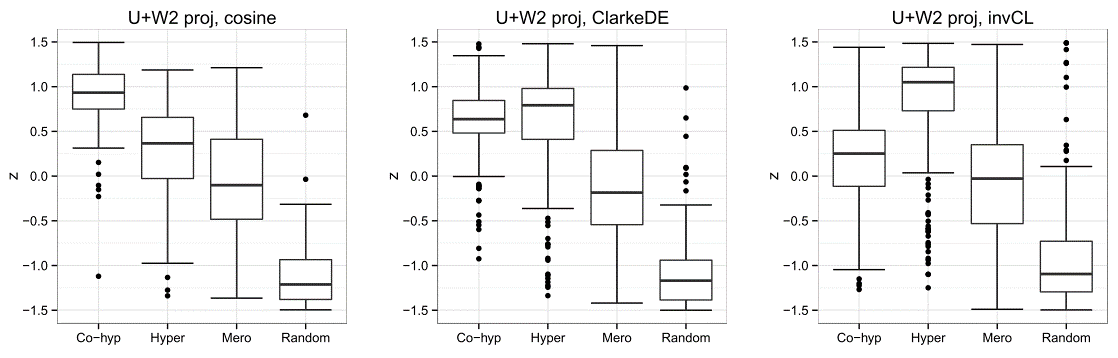
\includegraphics[width=1.\linewidth]{images/std_distrib_invCL_post_feature_selection.png}
  \caption{Standardised distribution of $cosine$, $ClarkeDE$, $invCL$ score across relations in \textit{U+W2} VSM, after feature selection \citep{roller2014inclusive}.}
  \label{fig:std_invCL_boxplot_500dim}
\end{figure}
The unsupervised measures were tested on the lower dimensional \textit{U+W2} vector space using the BLESS dataset.  We reproduced the figure from \citep{roller2014inclusive} in Figure~\ref{fig:std_invCL_boxplot_500dim}
Using the selected dimensions, the $ClarkeDE$ and $invCL$ measures return a higher standardised score for the hypernym term.  As expected, the $cosine$ symmetric measure was unaffected by the updated vector space and assigned a higher score to co-hyponyms.  Statistically significant results were, however, only achieved by the $invCL$ measure \citep{roller2014inclusive}.

\subsection{Unsupervised Measures as Features for Supervised Learning}
\citeauthor{santus2016nine} created another supervised-unsupervised hybrid system by using the scores emitted from various unsupervised measures as input features to several classifiers.  They originally selected thirteen unsupervised measures which are designed to capture different distributional properties of the word-pair vectors.  Feature selection was carried out by systematically excluding one feature at a time and looking at the impact on the model trained on the reduced feature set in terms of the $10$-fold cross-validated $F1$ score.  Through this exercise, four unsupervised metric features were dropped, reducing the set to nine features which included:
\begin{itemize}
    \item Target-word frequency and entropy for each word in the pair (4 features);
    \item The top $N$ context frequency and entropy for each word in the pair (4 features); 
    \item A symmetric measure called $APSyn$ \citep{santus2016unsupervised} (1 feature);
\end{itemize}
 
The supervision was provided by the \textit{ROOT9} dataset, consisting of $9,600$ pairs randomly extracted from \textit{BLESS} \citep{Baroni2011}, \textit{EVALution} \citep{santus2015evalution}, and \textit{Lenci/Benotto} \citep{benotto2015distributional}.  The word-pairs included verbs, nouns and adjective and spanned three semantic relations: co-hyponymy, hypernymy, random.  The vector space model was built from the same corpora as in \citep{santus2014chasing} with the following differences: the window-based context consisted of five words on either side of the target word; \ac{PPMI} was used to weight the feature association; only words which occurred in the joint corpus a minimum of 1,000 times were considered.  This last decision had some ramifications when the authors wanted to test their solution on the alternative \textit{Weeds} dataset \citep{weeds2014learning} since no vectors were available for several words in that dataset.

The authors performed a  battery of experiments.  The best-performing classifier was a multi-class random forest model, trained to detect whether a given word-pair is bound by co-hyponymy, hypernymy or is entirely unrelated.  With $10$-fold cross validation, an $F1$ class average of 0.907 was recorded.  Several baselines which included the use of alternative classifiers such as logistic regression, or different feature sets (cosine similarity measure, randomly initialised numbers between 0 and 1) recorded much inferior results (0.572 and 0.334 respectively), which supported the case that the random forest setup was especially effective.  

However, the result was not replicated when the same random forest model was evaluated on the \textit{Weeds} dataset \citep{weeds2014learning}.  Specifically, it struggled to correctly classify word-pairs featuring hypernymy, co-hyponymy and other relations extracted from WordNet \citep{Miller1995}.  This is not a coincidence: the \textit{Weeds} dataset was designed to eliminate the repetition of words in both the hyponym and hypernym word-pair slot.  Indeed, each word will feature at most twice: once as a hyponym and one other time as a hypernym.  This reduces the impact of hypernym memorisation \citep{levy2015supervised} since a classifier will not be exposed to enough examples of common hypernyms to provoke overfitting.  Similar lower results when evaluating on \textit{Weeds} were observed in other work \citep{shwartz2017siege}.

To test how sensitive their model is overfitting to prototypical hypernyms, \citeauthor{santus2016nine} devised a simple experiment which was replicated with the same outcome in other work \citep{shwartz2017siege}.  False hypernym pairs were generated by linking a hyponym with another word’s hypernym.  The \textit{ROOT9} classifier was evaluated on a dataset consisting of 3,200 switched hypernyms and the results reflected the severity of the problem:  up to 100\% of the hypernyms were falsely classified as hypernyms, if they also featured in the training set associated with one of its actual hyponyms.  \citeauthor{santus2016nine} mitigated this problem by enriching the random pair negative examples in the training set with switched hypernym word-pairs.  Although the $F1$ score plummeted by seven percentage points on the $10$-fold cross-validated test, only 546 random pairs were falsely classified as hypernyms.

In the next section, we will introduce word embeddings, a neural model driven mechanism to learn latent, low-dimensional vector representation of words which were used to provide features for other supervised solutions.

\section{Word Embeddings}
\subsection{Embeddings Overview}
To be included...
\subsection{Supervision with Word Embeddings} \label{supervised_embeddings}
The dense, low-dimensional word representations created with word embeddings methods make ideal features with which to train supervised classifiers.  \citep{shwartz2017siege} mounted a large, comparative experiment to study how well word embeddings features can help distinguish hypernymy from other semantic relations.  They experiment with pre-trained embeddings of various dimensionality, created by three models: word2vec skip-gram \citep{mikolov2013distributed}; GloVe \citep{pennington2014glove}; trained on dependency contexts \citep{levy2014dependency}.  For each embeddings space, the authors combined the term and candidate hypernym vectors using \textit{concat}enation \citep{baroni2012entailment} and \textit{diff}erence \citep{roller2014inclusive} vector operations.  The combined embeddings features were fed into two logistic classifiers, regularised with $L1$ and $L2$ terms.

\citeauthor{shwartz2017siege} train their supervised classifiers on the same four datasets upon which they tested an assortment of unsupervised measures, discussed in section \ref{shwartz_unsupervised}.  The datasets were split randomly and lexically, the latter following \citeauthor{levy2015supervised} recommendation to avoid lexical memorisation \citep{levy2015supervised}.  The scores were measured using \ac{AP} calculated on the top 100 most confidently predicted hypernyms ($AP@100$).

The classifiers’ performance on the randomly-split datasets is close to perfect ($1.0 <= AP@100 >= 0.873$) on all datasets with vector concatenation of GloVe embeddings driving the best results.  Similar to \citeauthor{levy2015supervised} findings, the high scores are influenced by \say{lexical memorisation} to some degree.  Indeed, the worst result was observed when evaluating the \textit{Weeds} \citep{weeds2014learning} dataset, which is designed to avoid memorisation by featuring each of the words $(x, y)$ exactly once in the $x$ or $y$ position.  However, hypernymy was still correctly predicted 87.3\% of the time on the Weeds dataset, suggesting the classifiers were able to home in on some features in the word vectors beyond the word itself.

Furthermore, \citeauthor{shwartz2017siege} discover that the overall performance of the classifiers is not overly penalised when the classifiers were trained on the lexically-split dataset.  They blame \citeauthor{levy2015supervised} poor results on lexically-split data on a shortage of training pairs, seeing that they sacrificed 50\% of the pairs to obtain a perfectly split dataset.  On their part, \citeauthor{shwartz2017siege} discarded only around 30\% of the pairs.  Thus, the authors are less sceptical about supervised methods’ ability to abstract away from words than \citeauthor{levy2015supervised} who posit that supervision merely recalls often-seen “prototypical” hypernyms in the training set.

Having said that, \citeauthor{shwartz2017siege} do not dispute that supervised methods are not able to capture relational features which tie the hyponym and hypernym words together.  The authors manipulated the dataset to introduce false random hypernyms by allocating true hypernyms to unrelated words as previously done in \citep{santus2016nine, levy2015supervised}.  The results, this time, paint a bleaker picture whereby the best supervised model drops 42 points to 0.575 $AP@100$ score.  However, unsupervised methods were unaffected by the same random hypernym dataset and actually improve by a small fraction.  The experiment highlights the robustness of unsupervised methods backed as they are by linguistic hypotheses and agnostic to lexical patterns embedded in a training set.  The authors suggest that unsupervised methods should be considered even when training data is available. Moreover, they can mutually benefit supervised methods as we have seen in previous work \citep{roller2014inclusive, santus2016nine}.

\subsection{Integrating Word Embeddings with Path-based Approach}
Recall \textsc{HypeNET} from section \ref{HypeNet}, the system created in \citep{shwartz2016path} which generates generalised hypernymy dependency paths using an \ac{LSTM} \citep{hochreiter1997long} encoder. The authors improved their path-only model by concatenating term and candidate hypernym word embeddings to either side of the averaged path vector.  The word vectors were furnished by GloVe pre-trained embeddings trained on a Wikipedia corpus \citep{pennington2014glove}.

To create the dataset, they followed \citep{Snow2004} by extracting directly related positive and negative instance from a variety of knowledge resources.  The latter included WordNet \citep{Miller1995} and YAGO \citep{suchanek2007yago}.  Since the solution employed dependency paths, only word-pairs that jointly occurred in the Wikipedia corpus, and which were connected by at least two unique paths were selected.

Similar to \citep{levy2015supervised}, \citeauthor{shwartz2016path} split their dataset both randomly and on a lexical basis.  The model trained on embeddings and path-based features yielded improved results compared to the path-based model and various supervised models constructed in the manner described in \ref{supervised_embeddings}.  The integrated model scored a 0.7 $F1$ score on the lexically-split dataset, marking a 6.1\% and 9.9\% improvement on the path-based and best supervised classifier respectively.  A 0.90 $F1$ score was attained on the randomly-split data by the integrated model -  a more marked improvement of 18.4\% and 20.8\% on the path-based and best supervised classifier respectively.  In all mentioned cases, the integrated model's superiority was statistically significant at a confidence level of 99\% according to the paired \textit{t-test}. 

In the next section, we will review a new family of supervised learning algorithms.  These algorithms learn a transformation matrix which projects the hyponym vector to a vector close to its hypernyminimising
the mean squared error or binary cross entropy objective function.  Such models enable hypernyms to be \textit{generated} rather than merely identified and are particularly amenable to the challenge outlined in SemEval 2018 Task 9 shared task \citep{camacho2018semeval}.

\section{Hypernym Discovery and Projection Learning}
In \citep{camacho2017we}, the author lamented the fact that no effort was spared to devise methods to identify hypernyms but notes that hypernym identification is limited in usefulness.  More effort needs to be poured in hypernym discovery, whereby a system generates hypernyms from the input features of a word-pair.  

However, most of the methods we reviewed so far were designed to map an input word-pair to an unsupervised score or supervised class label.  The supervised model returns the most probable semantic class a word-pair belongs to, according to the model’s learned parameters.  The unsupervised score is harder to interpret.  A higher score suggests a higher degree of hypernymy but a threshold needs to be found, across which a word-pair can be considered to be linked by hypernymy.  

Unsupervised methods can be used in a hypernym discovery setting as they were in the SemEval 2018 Task 9 unsupervised baselines created for the task \citep{camacho2018semeval}.  Given some bounded vocabulary, different words can be plugged in the measures’ $y$-word slot and the words returning the highest score returned as potential hypernyms.  On the other hand, the supervised methods we have seen so far – possibly with the exception of \citep{Snow2004} – were shown to suffer from lexical memorisation which would “discover” the most prominent hypernyms encountered in a training set irrespective of the query term.    Discovering hypernyms from Hearst patterns is viable \citep{hearst1992automatic, wu2012probase, Snow2004} but the assumption that hypernyms and hyponyms have to co-occur in the sentence will limit these methods’ coverage.  

\begin{figure}[ht!] 
  \centering
  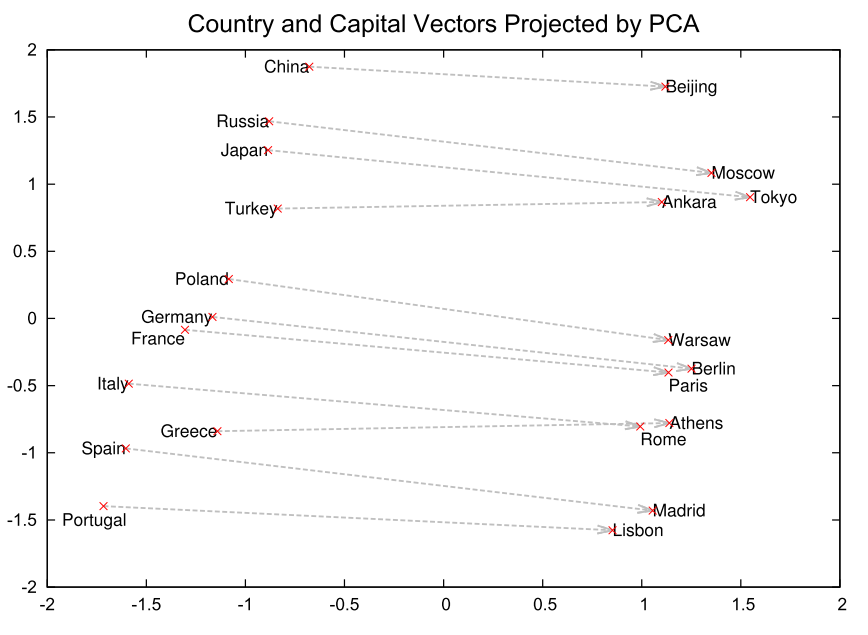
\includegraphics[width=1.\linewidth]{images/mikolov_semantic_regularity.png}
  \caption{Linear regularities between country and capital city retained in word embeddings from \citep{mikolov2013distributed}.}
  \label{fig:mikolov_capital_cities}
\end{figure}

\subsection{Early Work}
Word embeddings do not only represent word with continuous low-dimensional vectors but also retain semantic regularities in the vector space.  Figure~\ref{fig:mikolov_capital_cities} is reproduced from \citep{mikolov2013distributed} and illustrates the linear relationship between countries and their capital cities, after the distributional space is reduced to two dimensions using \ac{PCA}.  \ac{PCA} is a dimension reduction technique that reprojects the original features onto orthogonal axes (referred to as \textit{eigenvectors}) while still trying to capture most of the variance in the data.

Embedding offsets somewhat capture the relationship between words.  \citep{Fu2014} observe that the same phenomenon also applies to hyponyms and their hypernyms: vector offsets between hyponyms and hypernyms in similar domains were found to be similar.  Thus, the hyponym vector can be projected to its hypernym by applying a linear transformation.  Since it is unfeasible to calculate a separate linear projection for every hyponym, the authors propose learning an approximate projection $\bm{\Phi}$ which brings the dot product $\bm{\Phi} \cdot \bm{x}$ as close as possible to its hypernym $\bm{y}$.  Finding the optimal $\bm{\Phi}$ for our feature vector $\bm{x}$ requires the vector equivalent of scalar linear regression and can be approximated using the \ac{MSE} objective function:
\[\hat{\bm{\Phi}} = \argmin_{\bm{\Phi}} \frac{1}{N} \sum_{(x,y)} \Vert \bm{\Phi}\cdot\bm{x} - \bm {y} \Vert^2 \]

Stochastic gradient descent was the optimizer used to converge to the best solution for $\bm{\Phi}$ which returns the lowest average error over the training set.  The input word $\bm{x}$’s vector dimensions and $\bm{\Phi}$'s dimensions must be compatible to allow the dot product to be evaluated.  In general, $\bm{x}, \bm{y} \in \mathbb{R}^{d \times 1}$ represent the embeddings where $d$ is the embeddings dimensionality (typically between 50 and 300).  Therefore, the projection square matrix is $\bm{\Phi} \in \mathbb{R}^{d \times d}$ and the projected hypernym is $\bm{\Phi} \cdot \bm{x} \in \mathbb{R}^{d \times 1}$, which has the same dimensionality as the embeddings.  This allows it to be subtracted from the hypernym embedding $\bm{y}$ and the $L2$ norm can be computed on the vector offset to determine the distance between the estimated and the actual hypernym.  

The embedding vector space is too wide to expect any hyponym and its hypernym to have similar offsets.  In fact, $\bm{y}_{dog} - \bm{x}_{police\_dog} \approx \bm{y}_{fish} - \bm{x}_{tropical\_fish}$ but $\bm{y}_{dog} - \bm{x}_{police\_dog} \not \approx \bm{y}_{actor} - \bm{x}_{clown}$ \citep{Fu2014}.  \citeauthor{Fu2014} find that embeddings vector offsets make suitable dimensions for a clustering algorithm and they adapt the standard \ac{MSE} equation to a piecewise linear projection function:
\[\hat{\bm{\Phi}_k} = \argmin_{\bm{\Phi}_k} \frac{1}{N_k} \sum_{(x,y) \in C_k} \Vert \bm{\Phi}_k \cdot \bm{x} - \bm {y} \Vert^2 \]
The clusters are learnt using the unsupervised $k$-means algorithm, where the optimal $k$ is tuned on a validation set.  The clustering algorithm is fitted on the (hypernym – hyponym) vector offset which partitions the training data into distinct, semantically-related clusters.  Subsequently, a projection transformation matrix is learnt for the samples in each cluster.  Unseen pairs are first allocated to a cluster by transforming the vector offsets of their hypernym and hyponym representation using the $k$-means model fitted on the training data.  Hypernyms are discovered by first applying the learnt transformation matrix on the hyponym vector through the dot product operation, choosing the appropriate projection matrix based on the cluster assigned to the testing pair.  The closest neighbours to the estimated hypernym in the embedding space can then be found by cosine similarity or by dot-product if the vectors are first normalised to unit-length.

\citeauthor{Fu2014} do not cast the task as hypernym discovery, choosing instead to evaluate their solution within the familiar hypernym identification frame.  They focused on the Chinese language, starting from learning word embeddings from a 780-million word Chinese encyclopaedia corpus (Baidubaike) using word2vec’s skip-gram strategy \citep{mikolov2013efficient}, obtaining $560,000$ word embeddings.  $15,247$ training word-pairs were collated from \textit{CilinE}, a Chinese semantic thesaurus.  The evaluation set was sourced from the embeddings corpus and manually labelled by two annotators, ultimately settling on $1,391$ word-pairs which achieved an inter-annotator agreement score of 0.96.  One fifth of the evaluation set was retained as a development set.

The authors classify a word-pair $(x, y)$ as hypernymy as follows. They first assign a cluster to a word-pair, based on the cluster centroid which is closest by Euclidean distance to the vector offset $y - x$.  A positive match is found either: i) if the \ac{MSE} between the estimated hypernym and actual hypernym does not exceed a set threshold; or ii) if the estimated hypernym is close to another word $z$ such that is $z$ is a hyponym of the hypernym $y$, thus linking $x$ and $y$ through transitivity.

The $k$ number of clusters was tuned using the aforementioned development set, with the best performance recorded with 20 clusters and corresponding linear transformation matrices.  \citeauthor{Fu2014} measured performance using precision, recall and $F1$ score and their embeddings-based solution scored 80.54, 67.99 and 73.74 respectively.  A classification error analysis revealed that linear transformations could not be learnt if cosine similarity between the hyponym and hypernym in the embedding space exceeded 0.9038.  The authors reflect that having several training examples of this type could alleviate the problem.

\subsection{Negative Sampling}
The family of algorithms which learn a transformation matrix via stochastic gradient descent was coined \textit{projection learning} by 
\citeauthor{ustalov2017negative} who introduced the notion of negative sampling to \citeauthor{Fu2014}'s method \citep{ustalov2017negative}.  They observed that, normally, datasets used to train supervised models include both positive and negative examples.  Since a word’s nearest neighbours in the embedding space can be linked to the word via several semantic relations, the projection learning model must be shown examples of non-hypernymy to nudge the linear projection matrix away from projecting hyponyms to their synonyms, co-hyponyms, random words or back to the original hyponym.  However, unlike the binary cross-entropy objective function used in logistic classification, an \ac{MSE} loss function cannot deal with negative examples in the training set.

\citeauthor{ustalov2017negative} devise a number of regularisation terms which can be optionally added to the original \ac{MSE} objective function and minimised together.  The regularisation term is weighted by a constant $\lambda$ hyper-parameter which allows the experiment-taker to control how much importance is allocated to the regularisation term:
\[\hat{\bm{\Phi}} = \argmin_{\bm{\Phi}} \frac{1}{\vert P \vert} \sum_{(x,y) \in P} \Vert \bm{\Phi}\cdot\bm{x} - \bm {y} \Vert^2 + \lambda R\]

The regularisation terms reflect two main linguistic constraints.  In the first instance, the authors want to reinforce the asymmetric nature of hypernymy.  Applying the projection matrix back on to $\bm{\Phi} \cdot \bm{x}$ should not generate a vector similar to the original hyponym vector x and is penalised accordingly.  This option is ideal if no negative examples are available since we only require the hyponym itself to manage the regularisation term.
\[R = \frac{1}{\vert P \vert} \sum_{(x,) \in P} \big( \hat{\bm{y}} \bm{\Phi} \cdot \bm{x} \big)^2  \]
In the equation above, the regularisation term $R$ become larger the more similar the re-projected vector and the hyponym vector are. 

The second regularisation variant \citeauthor{ustalov2017negative} propose corrects the transformation matrix from projecting the hyponym to a semantically-related word that is not hypernymy.  The authors refer to this regularisation class as \say{neighbour regularisation} and use synonyms of hyponyms as the set of negative examples $N$, but other semantic relations are also valid as are randomly unrelated words.
\[R = \frac{1}{\vert N \vert} \sum_{(x,z) \in N} \big( \hat{\bm{y}} \bm{\Phi} \cdot \bm{z} \big)^2\]
Variants of the regularisation terms that are not reliant on re-projection were also included in the study.  The authors mounted experiments in the Russian and English language although we will focus mostly on the latter since English is the language of interest in this research project.

\citeauthor{ustalov2017negative} followed the methodology we have explored so far when working on the Russian language by converting a corpus into a vector space model, in this case opting for skip-gram word embeddings using the word2vec algorithm \citep{mikolov2013efficient}.  However, they departed from convention when working on the English language, by using 300-dimensional word embeddings pre-trained on the 100-billion token Google News corpus \citep{mikolov2013efficient}.  The projection learning model with additional regularisation terms was trained on a combination of four commonly-used datasets: \textit{EVALution} \citep{santus2015evalution}; \textit{BLESS} \citep{Baroni2011}; \textit{ROOT09} \citep{santus2016nine}; and \textit{K\&H+N} \citep{necsulescu2015reading}.  Each dataset features word-pairs linked together by an assortment of semantic relations.  The word-pairs linked by hypernymy constitute the positive pairs while the other semantic relations were used to provide \say{neighbour regularisation} example terms.  

The authors followed previous work \citep{levy2015supervised, shwartz2017siege, santus2016nine, roller2014inclusive} by performing a lexical split on the Russian dataset, but do not follow suit with the combined English dataset.  Since pre-trained word-embeddings are used, words which don’t have corresponding embeddings were discarded.  The dataset was ultimately split to 4,374 training pairs, 1,540 testing pairs and 1,483 validation pairs.  Synonyms and co-hyponyms were available for 1,314 terms, with each hyponym having between 1 and 39 relata.  The clustering mechanism used in \citep{Fu2014} is followed in \citeauthor{ustalov2017negative}’s work whereby the optimal number of clusters is tuned on the validation test, the training examples are allocated to their respective cluster based on the vector offset $y - x$, and a projection matrix is learned piecewise for the word-pairs in each cluster.  The best results on the combined English datasets were observed with 25 clusters.

In contrast to \citep{Fu2014}, \citeauthor{ustalov2017negative} framed the problem as a hypernym discovery task and evaluated the results accordingly.  Instead of precision, recall and $F1$ scores, they opted for $hit@l$ (similar to $precision@k$) and \ac{AUC}.  The authors chose to evaluate at $l=(1, 5, 10)$.  While $hit@l$ simply returns the average ratio of correct results in the first $l$-slots, \ac{AUC} also considers the rank of the predicted hypernyms.  The results they achieved showed that the regularisation terms added to the \ac{MSE} loss function improved the scores achieved on all metrics and across the English and Russian datasets, irrespective of the number of clusters trained.  

However, the improvement margin between the scores achieved with and without regularisation (controlling for the number of clusters), is slight.  Statistical significance (or otherwise) was not reported in their paper but the percentage improvement between the baseline score and highest score achieved by any one of the regularisation options is, on average, 1.3\%.  Regularisation terms had a greater impact on the single cluster model, where a 13\% improvement on the baseline was recorded.  However, in general, much better results were accomplished with the 25 cluster model which is consistent with \citeauthor{Fu2014}'s findings.

\subsection{Sense Awareness and Domain Clustering}
\citeauthor{espinosa2016supervised} contribute several developments to the projection learning research with their \textsc{TaxoEmbed} framework \citep{espinosa2016supervised}:
\begin{enumerate}
    \item They used a large sense-annotated repository to source the hypernym word-pairs; 
    \item They complemented the training set by unifying term-hypernyms pairs extracted from Open Information Extract (OIE) knowledge-bases;
    \item The embeddings are trained on a sense-annotated corpus which learns word-sense vectors;
    \item The clustering strategy is distinguished from previous attempts by partitioning the training space according to domain of knowledge rather than vector offset;
    \item They expand the partitioned training sets by exploiting the multiple lexicalisation words available for every concept;
\end{enumerate}

The sense inventory is provided by \textit{BabelNet} \citep{navigli2012babelnet}, a large multi-lingual, semantic repository encompassing both concepts and named entities and which is largely populated from knowledge embedded in Wikipedia and WordNet.  Like WordNet, words are organised in synsets containing one or more lexicalisations of words with the same meaning.  For instance the word (or lexicalisation) \textit{mole} is featured in 18 synsets among which:
\begin{itemize}
    \item The concept \say{spy who works against enemy espionage} sense (bn:00023221n) which includes the lexicalisations \textit{counterspy}, \textit{deep cover agent};
    \item The concept \say{molecular weight} sense (bn:00041297n) which includes the words \textit{mol}, \textit{gram molecule} as alternative lexicalisations;
    \item The named entity \say{Mole} (bn:03210051n) in the \textit{The Wind in the Willows} character sense;
\end{itemize}
The latest BabelNet 4.0 contains approximately 16 million synsets which are connected through semantic relations such as hypernymy, co-hyponymy, synonymy and so forth, extracted from WordNet.  Therefore, a hypernym of \textit{mole} in the espionage sense is \textit{spy} while in the \textit{molecular weight} sense, a hypernym is \textit{metric weight unit}.

\citeauthor{espinosa2016supervised} first mined 5.3 million hyponymy-hypernym synset pairs from the Wikidata branch of BabelNet and a further 1.35 million relations from various OIE knowledge bases.  The terms harvested from the knowledge bases are unaligned since they originated from different sources.  To resolve this problem, they leveraged the \textbf{KB-Unify} framework \citep{delli2015knowledge} to allocate the word-pairs into their corresponding BabelNet synsets and merge equivalent relations across disparate knowledge bases together.

Traditional word embeddings vectors represent words in surface-level form but the training pairs are expressed at the word-sense level.  For the sense embeddings, the authors employ \textsc{SensEmbed} \citep{iacobacci2015sensembed}, which represents word-senses in latent, continuous vector space.  The vectors were built by training word2vec \citep{mikolov2013efficient} on a sense-disambiguated version of Wikipedia, with each vector representing the concatenation of the word-form together with its corresponding BabelNet synset (ex: mole\_bn:03210051n).  In doing so, \textsc{SensEmbed} avoids the conflation of ambiguous homonyms into a single vector which results in a richer semantic space.   

The training word-pair clusters were not induced as in \citep{Fu2014, ustalov2017negative}; instead the content sections which separate Wikipedia’s featured articles \footnote{https://en.wikipedia.org/wiki/Wikipedia:Featured\_articles} by topic were used as cluster labels.  The authors reported 34 content sections (as at date of publishing), examples of which include \textit{Biology}, \textit{Food and Drink}, and \textit{Media}.  Each content section featured an average of 128 sample articles, chosen by Wikipedia as exemplary articles with respect to the high standards they met.  Training set terms were associated with a domain by creating a representative vector of each domain and then choosing the domain mostly associated with a synset via a lexical similarity metric.

The task was accomplished by leveraging \textsc{Nasari} \citep{camacho2016nasari} – a multilingual vector representation which represents words and their BabelNet senses in a joint semantic space.  Lexical domain vectors having words as dimensions, weighted by lexical specificity \citep{camacho2016nasari} were constructed from the concatenation of high-quality articles chosen by Wikipedia as representative of each domain.  Lexical specificity is a metric which returns the most representative words for a given text based on the hypergeometric distribution and is found to be superior to the conventional \ac{tf-idf} which was previously used to determine word relevance in a document \citep{camacho2016nasari}.  The similarity between each domain lexical vector and a training synset’s corresponding \textsc{Nasari} lexical vector was computed using Weighted Overlap (WO), a function that compares two vectors in terms of the rank of their overlapping dimensions.  The term synset was added to the domain whose vector returned the maximum WO score.

After domain clustering, the authors were able to augment the training set further by expanding the hyponym and hypernym sense concepts into their respective lexicalisations.  For example, new training pairs could be created by adding  \textit{counterspy\_bn:00023221n} and \textit{deep\_cover\_agent\_bn:00023221n} to the hyponym \textit{mole\_bn:00023221n}.  Similarly,  \textit{undercover\_agent\_bn:00073685n} was added to the  \textit{spy\_bn:00073685n} hypernym sense.  In this way, the original Wikidata and aligned OIE datasets were increased three and eleven-fold respectively.  

At this stage, a transformation matrix can be learned for each domain cluster by minimising \ac{MSE} similar to \citep{Fu2014}.  Like \citeauthor{ustalov2017negative}, \citeauthor{espinosa2016supervised} framed the task as a hypernym discovery problem.  They held out 250 test terms form each domain.  Finding potential hypernyms is more involved than \citep{ustalov2017negative} since the terms are expressed as BabelNet concepts rather than words.  Each test term concept is expanded to its lexicalisation vectors and the vocabulary words closest (by cosine similarity) to the dot-product of the cluster transformation matrix and lexicalisation vectors are found.  Each lexicalisation’s candidate hypernyms are ranked such that a condensed list of hypernyms can be returned for the lexicalisations’ sense concept.  Performance is evaluated on \ac{MAP}, \ac{MRR} and $precision@k$ .

In general, performance increased with training set size and having a mix of Wikidata and complementary \textbf{KB-U} training pairs.   Some domains such as \textit{Education}, benefitted particularly from a sizeable set of \textbf{KB-U} training pairs since the latter featured a large amount of \textit{is-a} knowledge about North American education institutions, which boosted the coverage of educational concepts.

Performance was also found to be influenced by the domain.  The best \ac{MAP} and \ac{MRR} scores were registered in the \textit{Biology} domain at 0.84 and 0.83 respectively.  The authors speculate that this was primarily due to the formal hierarchical division of flora and fauna, in itself an area of study that has been around for hundreds of years.  Lexical memorisation \citep{levy2015supervised} may have also had a part to play with the transformation matrix learning to project hyponym terms to prototypical hypernyms such as \textit{taxon}, \textit{vertebrate} and so on.   On the other hand, the \textit{Health} and \textit{Warfare} domains scored lowest with a maximum \ac{MAP} of 0.11 and 0.05 respectively; the \textit{Health} domain did not particularly benefit from an increase of training samples.  The authors do not provide reasons behind these (comparatively) poor results but one does suspect the opposite of the prototypical hypernym effect with a wide distribution of possible hypernyms that reduces any lexical memorisation advantage.

Finally, \citeauthor{espinosa2016supervised} demonstrate empirically the advantage of a piecewise projection matrix trained independently on a cluster of semantically related word-sense pairs.  When they introduced a large number of random pairs (hence, pairs which were not formally allocated a domain) to the various domains, the results were uniformly bad.  From all reported data, this results is a \ac{MAP} between 0 and 0.06, with the only outlier being the \textit{Biology} domain where a model trained on domain-unspecific sense pairs still managed a 0.81 \ac{MAP}.  Once again, this was attributed to the lexical memorisation phenomenon. 

\subsection{Joint-Learning of Clusters and Projection Matrices}
In contrast to the projection learning research we have examined so far, \citeauthor{yamane2016distributional} do not rely on the $L2$ norm between the projected hypernym vector and the gold-standard vector to measure how well hypernymy is being estimated.  Similarity, instead, is computed using the dot product of the unit-normalised estimated hypernym vector and actual hypernym embeddings.  The authors were directly motivated by the approach used in word2vec training \citep{mikolov2013efficient} whereby the similarity between the target word vector and context word vector was also computed by the dot product operation.  The similarity score is fed to a sigmoid function which estimates the probability that the projected hypernym vector is a good approximation of the word’s actual hypernym vector.  

The authors propose additional changes to the hypernym generation architecture.  The clusters are not allocated prior to training but are jointly learnt with the cluster parameters \citep{yamane2016distributional}.  Their model starts by creating a single cluster defined by the cluster parameters $\bm{\Phi}_1$,  a randomly-initialised projection square matrix, and a cluster scalar bias term $b_1$ initialised to 0.  The model computes the similarity $s$ with respect to a cluster $c$ for each word-pair $(x,y)$ in the training set according to the equation: 
\[s_c = \sigma\big( (\bm{\Phi}_c \cdot \bm{x}) \cdot \bm{y} + b_c \big)\]
If the maximum similarity for the training sample $(x,y)$ across all clusters does not exceed a threshold $\lambda$, the model assumes that none of the current clusters can adequately absorb the word-pair.  Thus, new cluster parameters are initialised and the word-pair is allocated to the new cluster.  Otherwise, if the maximum threshold is exceeded, the word-pair is allocated to the cluster yielding the highest similarity score. 

After a word-pair is mapped to a cluster, this cluster’s parameters are updated for the projection matrix and similarity measure.  Inspired by the negative sampling in word2vec, \citeauthor{yamane2016distributional} choose $m$ negative hypernyms $z$ of $x$ to discourage the model from projecting false hypernyms. The model’s ability to deal with negative examples is another novelty that distinguishes \citeauthor{yamane2016distributional}'s work from the pioneering effort of \citep{Fu2014}. The model learns the parameters by minimising the binary cross-entropy objective function across all $k$ clusters:
\[J(\bm{\Phi}; b) = \sum_{c=1}^{k} \sum_{(x,y) \in P_c} \Big[ -log \big(s_c(\bm{x}, \bm{y}) \big) - \sum_{i=1}^{m} log \big(1 - s_c(\bm{x}, \bm{z}_i) \big) \Big]\]
The authors experiment with Japanese and English, but we focus on English since it is aligned with our research.  Like \citep{ustalov2017negative}, the authors use readily-available English resources.  The word embeddings are pre-trained on the 100-billion word Google News corpus \citep{mikolov2013efficient} and the training, test and evaluation sets are the same \citep{baroni2012entailment} used in their experiments of supervised learning on lexical entailment.

The \citep{baroni2012entailment} dataset was partially derived from \textit{BLESS} \citep{Baroni2011} and included random pairs.  However, \citeauthor{yamane2016distributional} fed their model only positive examples since negative samples were generated on the fly during training.  Words having the highest cosine similarity to the hyponym vector $\bm{x}$ in the embeddings space were selected as negative samples.  The authors settled on a single negative example for every positive pair $(m=1)$.  The dataset was split such that 70\% of pairs were used for training, 25\% used for evaluation and 5\% used to tune the hyper-parameters such as $m$ negative samples and $\lambda$ similarity threshold.

Stochastic gradient descent was optimised by Adam \citep{kingma2014adam} where $\beta_1$, $\beta_2$ and the initial learning rate hyper-parameters were set according to the recommendations outlined in their paper.  Evaluation was performed on two levels.  Firstly, the joint-learning model with inner product similarity was compared to the “pipeline” model in \citep{Fu2014} which hard-clustered the terms prior to training and then learn piecewise projection matrices by minimising the mean square error objective function.  Secondly, the impact of multiple clusters on the performance was examined, but only on the Japanese dataset.  The English hypernymy dataset was roughly 6.5\% the size of its Japanese counterpart and probably not diversified enough for the model to learn more than two clusters. 

Unlike \citeauthor{Fu2014, espinosa2016supervised}, the test terms are not already allocated to a cluster prior to evaluation.  To determine the likelihood that a word $w$, taken from the embeddings space vocabulary, is a hypernym of a test term $x$:
\begin{itemize}
    \item Each cluster’s model forward-pass algorithm is invoked with inputs $\bm{x}$ and $\bm{w}$ to return the hypernym similarity between the two vectors;
    \item The similarity score for the candidate hypernym $w$ is the maximum score returned from all the cluster models;
    \item The words are ranked in descending order of maximum similarity score and the top $N$ candidates are emitted for evaluation;
\end{itemize}

\begin{table*}\centering
    \begin{tabular}{@{}lrrrrcrrrr@{}} \toprule
    & \multicolumn{4}{c}{\textbf{Development Set}} & \phantom{a} & \multicolumn{4}{c}{\textbf{Test Set}} \\ 
    & \multicolumn{2}{c}{\textbf{Japanese}} & \multicolumn{2}{c}{\textbf{English}} && \multicolumn{2}{c}{\textbf{Japanese}} & \multicolumn{2}{c}{\textbf{English}} \\ 
    %\midrule
    \cmidrule{2-5} \cmidrule{7-10}
    & \textit{Pipeline} & \textit{Joint} & \textit{Pipeline} & \textit{Joint} && \textit{Pipeline} & \textit{Joint} & \textit{Pipeline} & \textit{Joint} \\ \midrule
    \# Clusters & 1 & 1 & 1 & 1 && 5 & 19 & 1 & 2 \\
    \ac{MRR} & 0.215 & \textbf{0.279} & 0.321 & \textbf{0.343} && 0.193 & \textbf{0.349} & 0.280 & \textbf{0.339} \\
    \bottomrule
    \end{tabular}
    \caption{\ac{MRR} comparison between pipeline and joint models and cluster size \citep{yamane2016distributional}.}\label{tab:yamane_results}
\end{table*}

The authors focused on the joint-learning model’s ability to generate highly-ranked, correct hypernyms and opted for \ac{MRR} as evaluation metric.  We merge the results reported in the authors' paper in a single table, Table~\ref{tab:yamane_results} from \citet{yamane2016distributional}.

The \ac{MRR} yielded by the inner product model, proposed by \citep{yamane2016distributional} exceeds the “pipeline” model \citep{Fu2014} on both the Japanese and English development sets, controlling for a single projection matrix to focus on the effect of the objective function.  

Furthermore, \ac{MRR} was found to increase with the number of clusters and the joint-model showed the ability to learn higher-quality clusters than the pipeline model was able to induce from the $y-x$ vector offsets using the hard-clustering approach.  \citeauthor{yamane2016distributional}'s model was only able to learn two clusters over the English dataset, but this was enough to improve the \ac{MRR} score by 21\% over the best-tuned “pipeline” model.  When evaluating Japanese hypernymy, the authors controlled the number of learnt clusters by tuning the $\lambda$ threshold hyper-parameter.  \ac{MRR} increased with the number of clusters, hitting a peak (0.368) at 19 clusters after which performance gently decreased.  They also found that validation \ac{MRR} was unstable during the initial training epochs during which new clusters were created, and then proceeded to stabilise as the model settled on the optimal number of clusters.

\citeauthor{yamane2016distributional} do not examine the lexical memorisation bias especially in the English context where it was shown to be pronounced \citep{levy2015supervised, shwartz2017siege}.  Splitting the dataset on a lexical basis rather than on a random basis would have lowered the risk of learning prototypical hypernyms but, judging on previous studies, would have probably had an adverse impact on the model’s performance.

\subsection{CRIM Modifications to Yamane et al.}
The work submitted to Semeval 2018 Task 9 competition \citep{camacho2018semeval} by researchers affiliated with the \ac{CRIM} achieved the best scores in the English subtasks from all submitted solutions.  Several resources are provided by the task organisers including gold-standard datasets for each subtask and an extensive vocabulary to limit the candidate term search space.  The CRIM solution featured two components:
\begin{itemize}
    \item A supervised projection learning method using the inner-product vector operation to measure similarity between the projected and the actual hypernym embeddings, as introduced in \citep{yamane2016distributional};
    \item An unsupervised method which matches co-occurring hyponyms and hypernyms via the standard Hearst patterns \citep{hearst1992automatic} but which also leverages cosine similarity of their embeddings representation to assign a higher weight to words that are also distributionally similar to each other;
\end{itemize}

To increase recall in the unsupervised mode, the authors follow \citep{Snow2004, ritter2009anyway} and search for conjunction patterns in the corpus to harvest co-hyponyms $q'=(q'_1,\ldots,q'_k )$ of a given term query $q$.  The occurrence frequency of each co-hyponym $q'_i$ is recorded and a co-hyponym is scored by multiplying its occurrence frequency by the cosine similarity of $(q, q'_i)$.  The co-hyponyms are ranked by their score and the highest-scoring words are retained.  The harvested co-hyponyms are used to augment the mined hypernyms of $q$ since the coverage of the original hypernym is extended.  The hypernyms are ranked using the same method employed for the co-hyponym ranking.

In this section we will focus on \citeauthor{bernier2018crim}'s extensions to the inner-product similarity method introduced by \citep{yamane2016distributional}.  The authors’ most prominent deviation is opting out of clustering the training pairs as was done in the literature so far \citep{Fu2014, espinosa2016supervised, yamane2016distributional}.  Instead, they propose a trainable fixed tensor consisting of $k$ projection matrices $\bm{\Phi}_i \in \mathbb{R}^{d \times d}$ for $i \in \{1,\ldots,k\}$ where $d$ is the dimensionality of the embeddings.  Each linear projection matrix is applied to the hyponym embeddings to produce $k$ hypernyms projections $\bm{P} \in \mathbb{R}^{k \times d}$.  The vectors are normalised to unit length, and the similarity between each projected hypernym vector and the ground-truth positive or negative hypernym in the dataset is computed using the dot product.  The linear combination of $k$ similarity scores and $k+1$ weights (an intercept term is included) is fed to a sigmoid activation function which computes the probability that the training word-pair $(x,y)$ is linked by hypernymy.

The similarity weights and $k$ projection matrices are learnt by minimising the binary cross-entropy cost function.  Like \citep{yamane2016distributional}, they leverage Adam \citep{kingma2014adam} to optimize the gradient descent but override the recommended hyper-parameters by setting $\beta_1 = \beta_2 = 0.9$.

Apart from learning fixed multi-projection matrices, \citeauthor{bernier2018crim} carried out additional refinements to \citep{yamane2016distributional}.  They experimented with a projection matrix initialisation strategy whereby they added random noise - drawn from a normal distribution with mean 0 and stardard deviation set as per \citep{glorot2010understanding} - to an identity matrix.  Ablation experiments executed by the authors showed that this initialisation strategy helped the model achieve better results than when the projection matrices were just randomly initialised.

The authors also found that their model benefitted from a higher positive to negative sample ratio than an equal positive to negative ratio advocated in \citep{yamane2016distributional} where every training gradient update is based on a single positive and negative example.  The best results were observed when ten negative hypernym samples were drawn for every positive hypernm in the training set.  Moreover, down-sampling high frequency hypernyms had a positive effect when tuning their model on the development set but later tests revealed that scores would have been higher if the model was trained on all datapoints.  Notwithstanding, their official results were based on down-sampled runs.

\citep{yamane2016distributional} eschew regularisation entirely or do not report provisions taken in their publication.  \citeauthor{bernier2018crim} are aware of their model’s tendency to over-fit and add dropout to the word embeddings as well as the hypernym projection vector.  Furthermore, they use gradient clipping to avoid large gradient updates to the model in the back-propagation step, especially during the first training epochs and also employ early stopping to halt training once no improvement is observed on the validation set for a consecutive number of epochs.

The largest performance boost in the CRIM model was observed when the embeddings were fine-tuned.  The embeddings were initially pre-trained on each input corpus corresponding to the various sub-tasks, using the word2vec skipgram algorithm with negative sampling \citep{mikolov2013efficient}.  Prior to training the embeddings, the corpora were pre-processed such that bi-grams and tri-grams featured in the vocabulary were merged into an atomic token.  In all projection learning setups we considered so far, the embeddings weights are frozen and do not contribute to minimising the loss functions.  Training the embeddings specialises them for the task at hand, but could also result in the embeddings “forgetting” the semantic represenation learnt from the pre-training on the corpus, vastly limiting their usefulness \citep{howard2018universal}.  The authors do not report how the embeddings were tuned but ablation tests show that training the embeddings alongside the projection matrices and sigmoid layer weights improved the \ac{MAP} score by 45\% to 143\%, depending on which other features they excised from their model.

\begin{table*}\centering
    \begin{tabular}{@{}lrrrrcrrrr@{}} \toprule
    & \multicolumn{4}{c}{\textbf{Development Set}} & \phantom{a} & \multicolumn{4}{c}{\textbf{Test Set}} \\ 
    & \multicolumn{2}{c}{\textbf{Japanese}} & \multicolumn{2}{c}{\textbf{English}} && \multicolumn{2}{c}{\textbf{Japanese}} & \multicolumn{2}{c}{\textbf{English}} \\ 
    %\midrule
    \cmidrule{2-5} \cmidrule{7-10}
    & \textit{Pipeline} & \textit{Joint} & \textit{Pipeline} & \textit{Joint} && \textit{Pipeline} & \textit{Joint} & \textit{Pipeline} & \textit{Joint} \\ \midrule
    \# Clusters & 1 & 1 & 1 & 1 && 5 & 19 & 1 & 2 \\
    \ac{MRR} & 0.215 & \textbf{0.279} & 0.321 & \textbf{0.343} && 0.193 & \textbf{0.349} & 0.280 & \textbf{0.339} \\
    \bottomrule
    \end{tabular}
    \caption{\ac{CRIM} results achieved using projection learning only and hybrid results on the general-purpose English dataset \citep{bernier2018crim}.}\label{tab:CRIM_results}
\end{table*}

Like \citep{espinosa2016supervised}, \citeauthor{bernier2018crim} are aware that neural methods benefit from more training data, and tried to bolster their results by augmenting their dataset with synthetic examples.  They exploited word distributional similarity in the embeddings by finding a query’s nearest neighbour (measured by cosine similarity) in the embeddings space and considering that word a co-hyponym.  Similar to \citep{Snow2004, ritter2009anyway}, the authors assign the original query’s hypernym to the “synthetic” co-hyponym and include this as a new word-pair in the dataset.  Similarly, if two or more hypernyms share the same nearest neighbour, the latter is also considered a bona-fide hypernym, paired with the relevant hyponyms and added to the dataset.  

Amplifying the dataset had a positive effect on the results but only when combined with the unsupervised approach.  The synthetic examples had a slight detrimental effect on the projection learning supervised method.

    
    %% Commented out all chapters except into and background
    
    %%\chapter{Materials \& Methods}

\textbf{This section should include a recipe of what you did (explain what you have done so if someone wants to reproduce the experiment, they can).  A flow chart is typically helpful.  Also, make sure to define all software that you used including version numbers and OS.  Should also include a description of statistical methods used (if any).  \footnote{For more information see: \url{http://rc.rcjournal.com/content/49/10/1229.short}}}

\Blindtext
    %%\chapter{Results \& Discussion}
\textbf{Should include a reiteration of the experiments, and their outcome.  Together with a description (discussion).  Preamble should include a reminder of the aims and objectives together with a list of experiments to achieve these.  Should include many charts and other visualization with appropriate descriptions}.  

\Blindtext
\section{Some Other Section}
\Blindtext
    %%\chapter{Evaluation}
%%\textbf{In an ideal world, you should have two kind of evaluations.  The first is against some ground truth (perhaps a random model?).  The second kind of evaluation is against other people's work (accuracy, speed, etc.).  Any dimension which is of interest, should be evaluated.  Evaluation should be statistically sound. }
In this chapter, we interpret our experiment results against a backdrop of reviewed literature.  We divided our experiments in two parts.  In the first instance, we compared the reviewed projection learning techniques by evaluating them on a common dataset and evaluation metrics platform.  Each algorithm features specialised hyperparameters which - according to the original literature - were reported to have some influence on performance.  We built two out of the three algorithms from first principles, following the technical instructions in the respective papers \citep{ustalov2017negative, bernier2018crim}.  

We leveraged the \ac{ANOVA} framework to confirm or reject the hypothesis that a feature has no effect on score.  Before quoting the test's $F-$score and related $p-$value, we confirm that the three conditions for \ac{ANOVA} are met: normal distribution of the data points; homogeneity of variance; independent observations.  We use Jarque-Bera to test for normality; Omnibus to test for variance homogeneity; Condition Number to test for multicollinearity.  Whenever \ac{ANOVA} recommended that we reject the null hypothesis that the group means are equal, we ran Tukey \ac{HSD} post-hoc analysis which computes a series of pair-wise tests among the levels of a particular group to find out which factor levels have a significant effect on the model score.  We assume 95\% confidence throughout, which means we take a 5\% risk of committing a Type 1 error.

In the second set of experiments, we focused on our implementation of CRIM \citep{bernier2018crim} and applied the algorithm on the Shared Task \citep{camacho2018semeval}.  We motivated our decision by our experience in the previous set of experiments, where we found CRIM to perform well, was receptive to different embeddings and other settings, and was easy to train.  Moreover, it was the algorithm which yielded the highest scores in the English language tasks it was set out to solve in the actual shared task.  However, we apply a number of changes which enables us to reduce training epochs significantly (from an original range between 200 and 1000 to less than 20), particularly thanks to a simple transfer learning strategy we employ which lets us learn the projection matrices and tune the embeddings in two separate phases.

\section{Analyses of Projection Learning Models}
We split the evaluation in two, starting from an analysis of regularisation and cluster count on projection learning algorithms which are training by minimising \ac{MSE}.  We, also explore the effect of embeddings on projection learning, an analysis which, to our knowledge, has not been carried out by the research community.  In the second subsection, we focus on CRIM and Yamane, the models which leverage the dot-product to estimate the similarity between the predicted and actual hypernym, and which are trained to minimise the binary cross-entropy objective function.

\subsection{MSE Hard-Clustering Models}
We evaluate our results on the basis of five metrics, but we focus exclusively on \ac{MRR} and \ac{MAP} which provide two interesting facets of our discovered hypernyms: how highly the models ranks  the first correct hypernym; the average precision of our 15 generated hypernyms with respect to the gold standard.  We did not find \ac{MRR} and \ac{MAP} to be always correlated, according to Spearman's correlation test.

Inspired by the $F_1$ score, we fused the two scores by calculating the harmonic mean of the two metrics.  The harmonic mean averages the respective rates to give us a balanced metric which considers both aspects of a model's performance in one number, which we henceforth refer to as $M_1$.  This also saved time by avoiding having to run the analyses twice, once per metric.  We analysed three factors, each having the following levels:
\begin{itemize}
    \item Embeddings: word2vec, GloVe, fastText;
    \item Cluster: 1, 10, 25;
    \item Regularisation: Baseline, Asymmetric, Neighbour;
\end{itemize}

We wanted to investigate the effect of the factors' interaction on $M_1$ rather than the effect of each factor taken independently.  We decided to examine the interaction of cluster count and model for each embeddings space separately.  This was spurred by the fact that published results focused exclusively on word2vec embeddings which means we wanted to study the effect of cluster and baseline independently of the embeddings used.  We carried out a dedicated analysis of embeddings at a later stage.  

\subsubsection{Interaction Effect of Clusters with Regularisation}
We segregated our results per embeddings to get three sets of 45 $M_1$ observation each.  We started by examining the effect of clusters and regularisation on models trained on \textbf{word2vec} vectors.  A 2-way \ac{ANOVA} overall model testing for the effect of the interaction term on $M_1$ was significant, $F(8,36)=13.938$, $p \ll 0.05$.  However, we found the effect of the interaction between cluster and regularisation  insignificant.  After refitting the ANOVA model on the factors independently, we were not able to find statistical evidence that the effect of regularisation was significant.  On the other hand, the effect of clusters was significant on $M_1$, $F(2,40)=44.342$, $p \ll 0.05$, $\omega^2=0.637$.  Post-hoc analysis revealed that increasing the clusters from 1 to 10, 1 to 25 and 10 to 25 all had a positive effect on $M_1$ when training an MSE model on \textbf{word2vec} features.

In the case of \textbf{GloVe}, the overall \ac{ANOVA} model testing for the interaction of cluster and regularisation was not viable.  The regularised models were also found to be insignificant.  We refit the \ac{ANOVA} on the cluster effect only, which was found mildly significant, $F(2,42)=9.748$, $p < 0.05$, $\omega^2 = 0.280$.  Post-hoc analysis revealed that increasing clusters from 1 to 10 had a significantly negative effect on $M_1$, while increasing clusters from 10 to 25 had a positive effect.  However, increasing the clusters from 1 to 25 had no effect on the results.

Lastly, we tested the effect of clustering and regularisation on models trained on \textbf{fastText} embeddings.  Recall from our Results chapter, that fastText performance was inversely proportional to the number of clusters trained.  Neither the interaction of regularisation and clusters, nor regularisation alone had a significant effect on score.  Like word2vec and GloVe, the clusters factor had a moderately significant effect on $M_1$,  $F(2,42)=16.016$, $p \ll 0.05$, $\omega^2=0.40$.  Post-hoc analysis revealed that increasing clusters from 1 to 10, and from 1 to 25 has a significantly negative effect on $M_1$ while increasing clusters from 10 to 25 has a positive, albeit negligible, effect.  

\subsubsection{Interaction Effect of Clusters with Embeddings}
After evaluating the effect of regularisation and clusters on the embeddings separately, and finding  regularisation insignificant in every scenario, we examined the effect of the interaction between clusters and embeddings on $M_1$.  To run this test, we used the scores obtained on the baseline model, which implements the original projection learning algorithm proposed by \citet{Fu2014}.  The interaction of clusters and embeddings was found to be significant, most probably due to the fact that performance on word2vec improves with increasing clusters whilst the opposite happens with the other two embeddings. To discover how embeddings reacts with clusters, we executed three 1-way \ac{ANOVA}, one for each separate cluster count.  

We found embeddings to have a strong, significant effect on single-cluster baseline models, $F(2,12)=52.376$, $p < 0.05$, $\omega^2=0.876$.  Post-hoc analysis revealed that fastText vectors yield a higher $M_1$ score than GloVe, and that GloVe in turn return higher $M_1$ than word2vec.  The effect decreases but it still significant on 10-cluster models, $F(2,12)=9.471$, $p < 0.05$, $\omega^2=0.530$.  In this scenario fastText embeddings mean scores are significantly higher than both word2vec and GloVe but GloVe results are not significantly better than word2vec.  Finally, we see the gap narrowing in the 25-cluster scenario.  The effect of embeddings is still moderately significant, $F(2,12)=11.406$, $p < 0.05$, $omega^2=0.582$, but post-hoc shows that the only significant $M_1$ difference is observed when comparing fastText and GloVe, the latter being worse.  

\subsection{Binary Cross-entropy Models}
We evaluated our implementation of two models, CRIM and Yamane, both of which learn multiple projection matrices without resorting to hard-clustering.  We believe that hard-clustering runs counter to the philosophy of hypernym discovery.  The clusters are originally learned in an unsupervised fashion, by applying a $k-$means model to the hypernym/hyponym vector offsets.  To allocate the test samples to the clusters, the hypernym vector needs to be used to compute the appropriate vector offsets.  This is equivalent to leaking test data to the training procedure.  In reality, we should not assume, and do not require, the presence of test hypernyms when validating a hypernym discovery model.  CRIM and Yamane only need query terms, and a vocabulary to bound the search space, to estimate hypernyms and thus are "purer" hypernym discovery implementations.  We test CRIM on four factors each having the following levels:
\begin{itemize}
    \item Embeddings: word2vec, GloVe, fastText;
    \item Projections: 1, 5, 10;
    \item Negative samples: 1, 5, 10;
    \item Regularisation strength: 0, 0.1, 1.0;
\end{itemize}
Yamane, on the other hand, are tested on a single factor, embeddings.  At the end of this section, we compare the best-performing MSE, Yamane and CRIM models and test for statistical significant performance differences.  As we did in the previous section, we evaluate our results on a custom metric we dubbed $M_1$, which is the harmonic mean of \ac{MRR} and \ac{MAP}, which are numbers in the range $[0,1]$.  Once again, we leveraged \ac{ANOVA} to determine whether differences of means between factors were significant.

\subsubsection{Interaction Effect of Projections and Negative Sample Count on CRIM}
To reduce the complexity of \ac{ANOVA}, we temporarily ignored the regularisation factor and proceeded to examine the interaction of projections and negative samples on each embeddings space separately, starting from \textbf{word2vec}.  The overall model testing for the combined interaction was significant $F(8, 36)= 11.230$, $p<0.05$ but inspection of the \ac{ANOVA} table informed us that the mean difference due to the combined interaction was not significant.  We refitted the model, this time investigating the main effects separately.  The projection factor effect was found to be moderately significant on $M_1$, $F(2,40)=25.06$, $p < 0.05$, $\omega^2=0.410$; the negative sample factor was less significant, $F(2,40)=13.159$, $p < 0.05$, $\omega^2 = 0.207$.  We conducted post-hoc analyses on both factors. Increasing the negative sample count from 1 to 5 or from 1 to 10, was justifiable since both are expected to increase $M_1$. Performance does not increase significantly when the negative sample count is augmented to 10 from 5.  A stronger, negative significant effect was detected when the model learned several projections.  Increasing projection layers from 1 to 10, reduced the mean difference by 0.035 points, while a less pronounced, but nonetheless significantly, negative effect was estimated with 5 projection layers.

With \textbf{GloVe}, the combined interaction was not significant. However, the main effects were significant when tested independently.  The projection factor had a strong effect on $M_1$, $F(2,40) = 63.77$, $p \ll 0.05$, $\omega^2=0.714$ while the negative count also had a significant but much weaker effect, $F(2,40) = 3.70$, $p < 0.05$, $\omega^2 = 0.031$.  Post-hoc revealed that, contrary to the word2vec scenario, increasing the projections from 1 to 5 and from 1 to 10 pushed the $M_1$ score up by 3.81 and 4.25 points respectively.  Increasing projections from 5 to 10 had a positive but insignificant effect on the score.  Meanwhile, post-hoc analysis reported that the negative sample count had no significant effect on the ultimate score.

Once again, the combined interaction was significant for models trained on fastText vectors.  However, the negative sample count, and projection factor both had a significant, independent effect on $M_1$.  The negative count was significant, $F(2,40)=11.23$, $p < 0.05$, $\omega^2 = 0.212$; projections are significant, $F(2,40)=16.48$, $p < 0.05$, $\omega^2 = 0.321$.  Post-hoc analysis indicated that learning more than a single projection benefited fastText-trained models although going from 5 to 10 projections had an insignificant effect.  As far as negative samples are concerned, the cross-validated score increased significantly only when the model was trained on 10 negative samples.

\subsubsection{Interaction Effect of Projections with Embeddings on CRIM}
Next, we studied the combined and independent effect of projections and embeddings.  We only considered results from models trained with 10 negative samples.  At worst, 10 negative samples were found to have an insignificant effect on our models, so eliminating the negative sample factor should not have any effect on our analysis.  For this exercise, we set aside our regularisation modification and analysed results returns by unregularised models (i.e. regularisation weight $\lambda=0$).

The combination of embeddings and projections factors was significant, $F(4,36)=21.578$, $p \ll 0.05$, although the effect is very weak with $\omega^2=0.07$.  On the other hand, the independent effect of the embeddings is very strong with $\omega^2 = 0.88$.  We opted against exploring the embeddings independently since previous tests have shown projections to be often significant when examining embeddings spaces separately.  Instead we re-ran \ac{ANOVA} focusing on the simple effect of embeddings, by examining the three  projection levels separately.

The choice of embeddings exerts a large influence on the $M_1$ score of a single-projection CRIM model, $F(2, 12)=297.95$, $p \ll 0.05$, $\omega^2 = 0.97$.  Post-hoc analysis further revealed that fastText embeddings had a positive, significant effect on $M_1$.  The mean difference between fastText and GloVe was estimated at 12.2 points, in favour of fastText.  The latter tend to yield a higher $M_1$ than word2vec embeddings would but word2vec vectors are also significantly superior to GloVe.

We reached the same conclusion for 5-projection models.  Embeddings had a similarly strong effect on $M_1$ score, $F(2, 12)=163.24,$ $p \ll 0.05$, $\omega^2 = 0.956$.  Post-hoc analyses re-asserted our previous findings: fastText embeddings yield the best result while GloVe will be significantly worst.

The embeddings effect was also significant in models which learn 10 projections, $F(2,12)=152.53$, $p \ll 0.05$, $\omega^2 = 0.953$.  fastText embeddings are expected to increase $M_1$ by 10.35 points and 9.39 against GloVe and word2vec respectively.  However, the 10-projection, word2vec-trained CRIM model was sufficiently poor to be almost indistinguishable from a 10-projection model trained on GloVe word vectors.

\subsubsection{Interaction Effect of Regularisation and Projections}
In \cref{crim_model_structure}, we described our modification to the original CRIM model, whereby together with \textit{random} negative samples, we fed the model with 5 \textit{semantically-related} negative examples.  The mean similarity of the semantically-related words to the projected hypernym was added as a regularisation term in our customised loss function.  The importance the model assigned to this regularisation term is determined by the weight scalar $\lambda$ which takes on values in the range $[0,1]$, where 0 signals the model to ignore the regularisation term. 

The results were, generally-speaking, indifferent to regularisation.  In a few cases, the \ac{MAP} and/or \ac{MRR} scores increases fractionally, and in other cases dipped marginally.  We evaluated the influence of our three regularisation weighting settings by considering the embeddings separately.  We initially attempted to fit an \ac{ANOVA} model on the 4-way interactions of embeddings, projections, negative samples and regularisation weight but the overall model failed the multicollinearity test.  We encountered the same problem when testing for 3-way interactions, having eliminated the embeddings factor.  This forced us to follow a simpler evaluation strategy. 

We evaluated the combined and independent effect of projections and regularisation weight on word2vec and fastText separately \footnote{We did not evaluate regularisation with GloVe due to its significantly low performance when used with CRIM.}.  For each embeddings space, we fit separate models for every negative sample count settings.  The combined interaction was found to be weakly significant for a fastText model trained with 5 negative samples, $F(4,36)=3.271$, $p < 0.05$, $\omega^2=0.093$.  To find which particular factor combination was responsible for this, we tested for "between-subject" effects and found a significant effect of the regularisation factor on a single-projection model, trained on fastText vectors with 5 negative samples, $F(2,12)=4.290$, $p <  0.05$, $\omega^2=0.305$.  Post-hoc analysis showed a significant, negative difference of means when subtracting the mean result where $lambda=1.$  from $lambda=0.$.  In this scenario, regularisation damaged the models' prospects.

\subsubsection{Effect of Embeddings on Yamane}
We fit Yamane models with features extracted from our three embeddings spaces.  To test if the choice of embeddings is significant on Yamane's result, we performed a 1-way \ac{ANOVA} on the embeddings factor.  The effect was strongly significant on $M_1$, $F(2,12)=33.28$, $p < 0.05$, $\omega^2=0.81$.  As we had noted in the Results chapter, Yamane levels the fastText and word2vec performance.  Post-hoc revealed there is no significant difference between the score obtained from models trained on fastText and word2vec.  However, the use of GloVe embeddings led to a significant 9.37 point deduction from the $M_1$ returned by word2vec.

\subsection{Best Out of Three}
We selected the best model out of our \ac{MSE}, CRIM and Yamane categories to find out whether the difference in the means of cross-validated scores was superficial or significant.  We fit a 1-way \ac{ANOVA} which tests for differences on the model factor, which we found significant, $F(2,12)=11.390$, $p < 0.05$, $\omega^2=0.581$.  Post-hoc analyses found that both Yamane and CRIM were significantly better than the top \ac{MSE} model, returning a mean of 4.01 and 3.50 points respectively more than \ac{MSE}.  No significant difference was detected among CRIM and Yamane results.

\subsection{Analyses of Lexical Memorisation Effect}
Some hypernyms will invariably feature at a higher frequency than others.  Common hypernyms such as \textit{animal} and \textit{person} capture the \textit{is-a} relation of a large number of words.  Table~\ref{tab:high_freq_hyper_combined_set} features the 10 most frequently occurring hypernyms and 10 of the least frequently hypernyms in the combined dataset on which we trained our models during the first experiment phase.
\begin{table*}\centering
    \begin{tabular}{@{}lrclr@{}} \toprule
    \multicolumn{2}{c}{\textbf{Most Frequent}} & \phantom{a} & \multicolumn{2}{c}{\textbf{Least Frequent}}\\
    \textit{Word} & \textit{Frequency} && \textit{Word} & \textit{Frequency} \\ 
    \cmidrule{1-2} \cmidrule{4-5}
    animal & 0.06676 && attach & 0.00017 \\
    plant & 0.05947 && property & 0.00017\\
    chordate & 0.04863 && attitude & 0.00017\\
    vertebrate & 0.04812 && enemy & 0.00017\\
    mammal & 0.02762 && relationship & 0.00017\\
    placental & 0.02474 && aconite & 0.00017\\
    herb & 0.0205 && exist & 0.00017\\
    invertebrate & 0.01305 && handcart & 0.00017\\
    artifact & 0.01288 && educational & 0.00017\\
    artefact & 0.01288 && helpful & 0.00017\\
    \bottomrule
    \end{tabular}
    \caption{10 most frequent (l) and least frequent (r) hypernyms in combined dataset.}\label{tab:high_freq_hyper_combined_set}
\end{table*}
A word-pair drawn at random from the dataset is 393 times more likely to feature \textit{animal} in the hypernyms slot than, say, \textit{handcart}.  Of course, there are more hyponyms of \textit{animal} in the English language than there are of \textit{handcart}.  Splitting the dataset on a lexical basis is effective when classifying word-pairs as hypernymy or otherwise \citep{shwartz2017siege, levy2015supervised, santus2016nine}, but sharply depletes the training set and evaluation set pairs when applied to hypernym discovery.  Therefore, it is possible that a model might learn a transformation matrix which projects any word to a \textit{prototypical hypernym}.

Although our results, particularly when compared to the \ac{MFH} na\"ive baseline, do indicate that the model is learning some aspect of the linear relationship between hyponyms and hypernyms in the embeddings space, we wanted to investigate the degree to which scoring success is predicated by hypernym frequency.  In this exercise, we focus exclusively on the CRIM and Yamane binary cross-entropy models.  We wanted to eliminate the bias that \ac{MSE} models introduce by leaking test data into the model by clustering similar word-pairs together prior to predicting the hypernyms.

We fit a CRIM and Yamane model on the same training split and got each respective model to predict the hypernyms of query terms in the same test split.  We scored the \ac{AP} of the retrieved projections and found the median frequency rate of the corresponding gold-standard hypernyms \textit{in the training set}.  If none of the gold-standard hypernyms featured in the training set, we assigned a median score of 0. The results were charted in a scatter-plot to which we added random jitter on both axes to get a better sense of the bivariate relationship.  A regression line was fitted and superimposed on each plot.  Both plots can be seen in Figure~\ref{fig:scatter_crim_yamane}.
\begin{figure}[!ht]
    \centering
    \subbottom[CRIM]{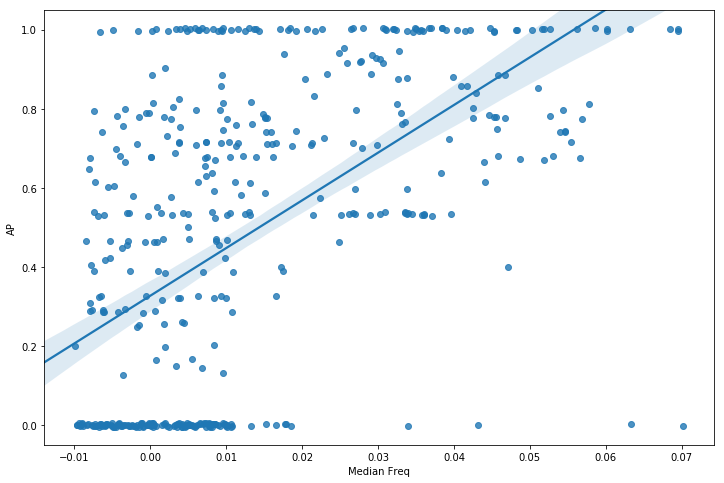
\includegraphics[width=0.5\textwidth]{images/scatter_crim.png}}\qquad
    \subbottom[Yamane]{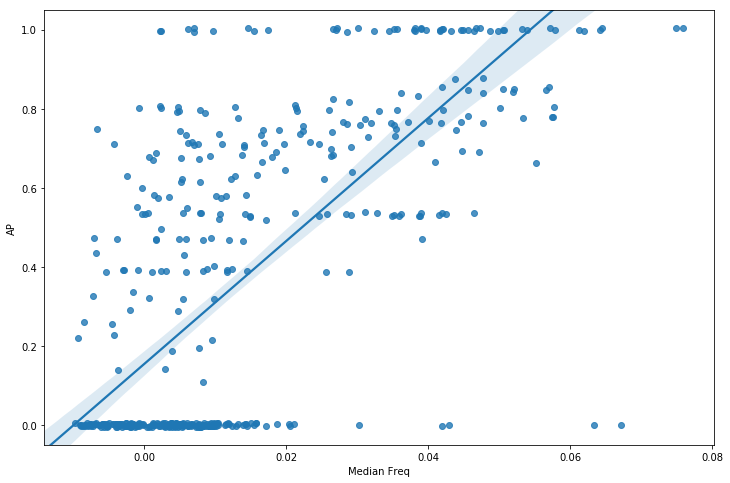
\includegraphics[width=0.5\textwidth]{images/scatter_yamane.png}}%
    \caption{Scatter-plot of median gold hypernym frequency against \ac{AP}.}        
    \label{fig:scatter_crim_yamane}
\end{figure}

There is a linear, positively-correlated relationship between the median frequency of the gold hypernyms which also feature in the training set and the precision of predicted hypernyms.\footnote{Note that query terms (i.e. hyponyms) feature in either the training set or test set but never in both.}  A cluster of points at the bottom-left of the charts represent query words which scored 0 \ac{AP}.  The model struggled to generate correct hypernyms on account of the absence of these words in the training set.  CRIM (top) shows more of a tendency to score well on seldom seen hypernyms, as attested by a larger concentration of point to the top-left of the plot than can be found in the same region of the Yamane plot.  The regression lines explain 0.31 and 0.51 of CRIM's and Yamane's hypernym frequency/score relationship respectively.  The median gold hypernym frequency has less predictive power in CRIM than in Yamane.  This might suggest that CRIM generalises more than Yamane, possibly due to the fact that gradient updates are computed on batches of 352 samples compared to just 6 samples in the case of Yamane.

Next, we investigated the negative hypernyms most often predicted with the highest confidence by each respective model, for query terms that yielded an \ac{AP} score of 0.  We plotted the 15 most common top-ranked, false positive words predicted by CRIM and Yamane respectively with histograms shown in Figure~\ref{fig:false_positive_crim_yamane}.
\begin{figure}[!ht]
    \centering
    \subbottom[CRIM]{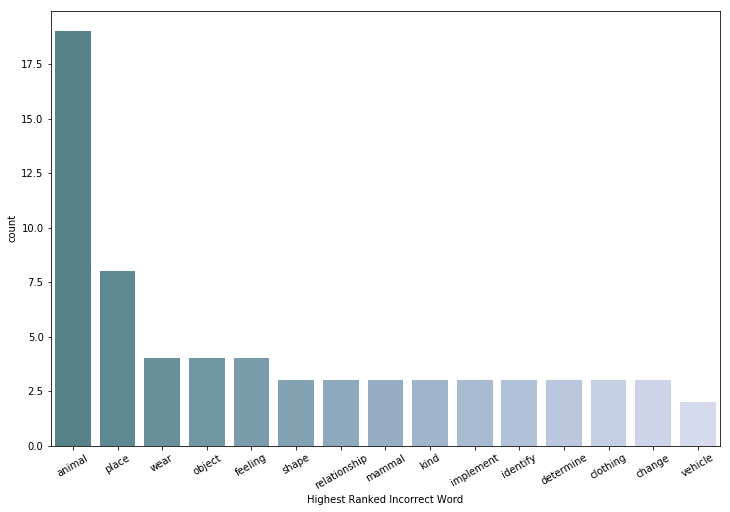
\includegraphics[width=0.6\textwidth]{images/crim_highest_ranked_incorrect.png}}\qquad
    \subbottom[Yamane]{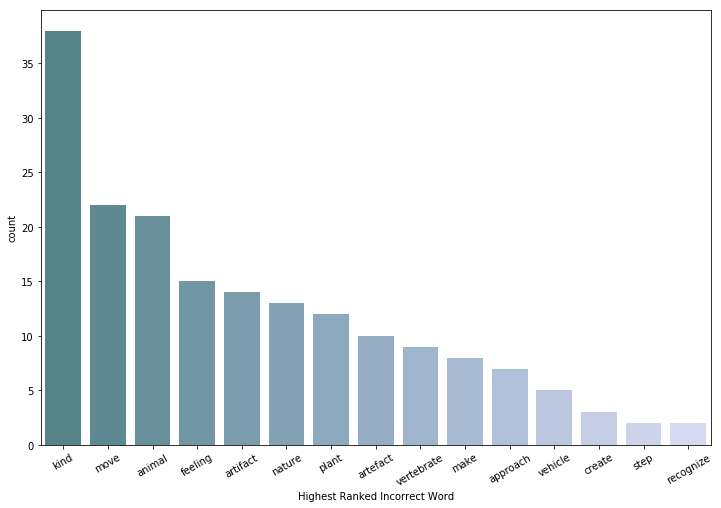
\includegraphics[width=0.6\textwidth]{images/yamane_highest_ranked_incorrect.png}}%
    \caption{Highest-ranked false positive hypernyms.}        
    \label{fig:false_positive_crim_yamane}
\end{figure}
Both CRIM and Yamane display a tendency to generate hypernyms which were often encountered during training such as \textit{animal}, \textit{plant} and \textit{object}.  Out of the 15 false positives most-commonly predicted by CRIM, two featured in the top ten highest occurring hypernyms in the training set. In the case of Yamane, five of these words were also on the top ten hypernym list.  Therefore, a shade of lexical memorisation can also be observed in projection learning models.  Perhaps, this phenomenon cannot be entirely avoided in the context of supervised learning.  

To restore some of our confidence in the capabilities of projection learning models, let us consider examples of terms which scored a perfect 1 \ac{AP}.  Moreover, we will only regard terms with hypernyms which seldom occur in the training set.  We will focus on CRIM, which has shown more ability to discover relatively rare hypernyms.  We reiterate that the length of the gold-standard list exerts a heavy weight on the scoring function we borrowed from the SemEval shared task \citep{camacho2018semeval}.  

\begin{table*}\centering
    \begin{tabular}{@{}lrrl@{}} \toprule
    \multicolumn{4}{c}{\textbf{CRIM Predictions}} \\
    \textit{Word} & \textit{AP} & \textit{Median Frequency} & \multicolumn{1}{c}{\textit{Top 5 Predictions}} \\ \midrule
    airship & 1. & 0.00373 & \textbf{vehicle}, \textbf{craft}, \textbf{aircraft}, airplane, artifact \\
    canoe & 1. & 0.00339 & \textbf{vehicle}, \textbf{boat}, \textbf{craft}, \textbf{vessel}, watercraft \\
    drape & 1. & 0.00271 & \textbf{cover}, wear, buy, sell, protect \\
    fog & 1. & 0.00085 & \textbf{weather}, change, place, shape, supply\\
    liberty & 1. & 0.00017 & \textbf{freedom}, liberty, belief, element, object\\
    square & 1. & 0.00119 & \textbf{shape}, place, form, figure, point\\
    violence & 1. & 0.00271 & \textbf{action}, violence, emotion, crime, anger\\
    yellow & 1. & 0.00237 & \textbf{color}, plant, crop, flower, green\\
    \bottomrule
    \end{tabular}
    \caption{Terms having low-frequency hypernyms correctly predicted by CRIM.}\label{tab:crim_perfect_score}
\end{table*}

Table~\ref{tab:crim_perfect_score} shows the top five hypernyms, predicted by CRIM \footnote{unregularised; 10 projections; 10 negative samples; trained on fastText word features for 15 epochs.}, for the terms having the least frequently occurring gold hypernyms.  Words in bold are gold-standard hypernyms and most terms in the table featured only a single gold-standard hypernym.  The model was unregularised, which explains why predictions at times include the term word itself (\textit{liberty}, \textit{violence}), or synonyms of the word (\textit{yellow}).  However, the model also surprises us with hypernyms which, despite being technically incorrect, are arguably precise.  Examples include, \textit{canoe} $\Rightarrow$ \textit{watercraft}; \textit{liberty} $\Rightarrow$ \textit{belief}; \textit{square} $\Rightarrow$ \textit{place}, \textit{form}, \textit{figure}; and \textit{violence} $\Rightarrow$ \textit{crime}. 

\subsection{Observations}

% CRIM is at least as good as Yamane
% Yamane's assertion that "joint learning" method is better "pipeline" model as he calls clustering together with piece-wise transformation matrix learning
% Choice of embeddings makes a real difference
% Increasing projections works, just on word2vec which is what bernier observed after running ablation tests
% during the shared task result evaluation
All configurations - irrespective of model, embeddings choice, clusters or regularisation comfortably beat the basic Cosine similarity and \ac{MFH} na\"ive baselines.  We did not evaluate these results statistically, since the improvement is obvious: for instance the fastText, single-cluster asymmetric model minimising \ac{MSE} beats the \ac{MFH} baseline by a 69\% margin.

With respect to the \ac{MSE} model family, there is strong empirical evidence which suggests that - on our chosen combined dataset and metrics - training a single-cluster, baseline model on fastText is the way to go.  We challenged the \citet{ustalov2017negative} assertion that regularisation has an effect on \ac{MSE} model performance.  Indeed, we found that regularisation has no significant effect on $M_1$ both in interaction with other factors, and in isolation.  This applied on all embeddings, including the same word2vec embeddings \citeauthor{ustalov2017negative} used in their English experiments.  However, we did not run an exhaustive grid-search tests to tune the $\lambda$ regularisation weighting parameter; instead we fixed the setting to 1, which was their chosen regularisation weight for re-projected regularisation.

\citet{Fu2014} findings were re-confirmed, despite the setup was modified in several ways: we recast their original problem as hypernym discovery; we evaluated on information retrieval metrics; we cross-validated the models on a different dataset.  Cluster size was certainly found to improve performance on word2vec embeddings, although the same did not hold for the other embeddings vector spaces, particularly fastText.

Introducing the regularisation terms proposed by \citet{ustalov2017negative} to a binary cross-entropy model (CRIM) did not really work out.  The effect was moderately negative, insofar that a significant result was only observed in one model setup out of 27.  Regularisation was not found to have any significant effect on \ac{MSE} models either.  

Increasing the projections in CRIM, had an adverse reaction when training the model on word2vec features.  \citet{bernier2018crim} reported a different empirical experience whereby multiple projections improved their \ac{MAP}/\ac{MRR} score.  This could be due to the interaction of the projection layer setting with one or several other setting.  The authors themselves specifically point out that they did not perform an in-depth analysis of their hyperparameter settings.  Moreover, they tune embeddings jointly with the projection matrices while decreasing the learning rate by a full order of magnitude and training for several hundred epochs.  

In both \ac{MSE} and binary cross-entropy model types, fastText was proven to be the superior embeddings out of the three tested.  We believe this is a small contribution we made to the research area since, to our knowledge, projection learning models have so far only been evaluated on word2vec embeddings features.  Yamane, on the other hand, narrowed the gap between word2vec and fastText we had so far observed.  Yamane and CRIM were found to perform significantly better than \ac{MSE} models which \citet{yamane2016distributional} refer to as \say{pipeline models}. In this paper, the authors reported the superior performance of the "inner product" method, an assertion we found to be statistically sound.

The poor performance of GloVe, is probably due to how the embeddings training algorithm makes use of the dot product operator.  In word2vec and fastText, dot-product is used to estimate the similarity of the context word and target word (and vice-versa depending on the model choice).  In GloVe the objective function encourages the dot product of word vectors to approximate the log of the co-occurrence probability of the words which may make the embeddings less suitable for our model.

\section{Experiments on Shared Task Corpus and Data}
Recall that we made exclusive use of our CRIM implementation when attempting the Shared Task.  We deliberately opted for the same metrics when evaluating the models on the Combined and Shared Task dataset.  This enables us to compare the performance of the same model on different data.  Doing so, we observed that the multi-projection model performed substantially better on the Combined Dataset.  For instance, a 10-projection CRIM model trained on fastText embeddings returned 0.391 \ac{MAP}; the equivalent model trained on the Shared Task dataset only managed 0.133 \ac{MAP}.

Despite the performance reduction with Shared Task data, two significant observations we made with the Combined Dataset still hold:
\begin{itemize}
    \item fastText embeddings still coax the best performance out of the CRIM model compared to word2vec and GloVe;
    \item Learning more than a single projection layer improves \ac{MAP} and \ac{MRR} performance;
\end{itemize}
\begin{figure}[!ht]
    \centering
    \subbottom[MRR]{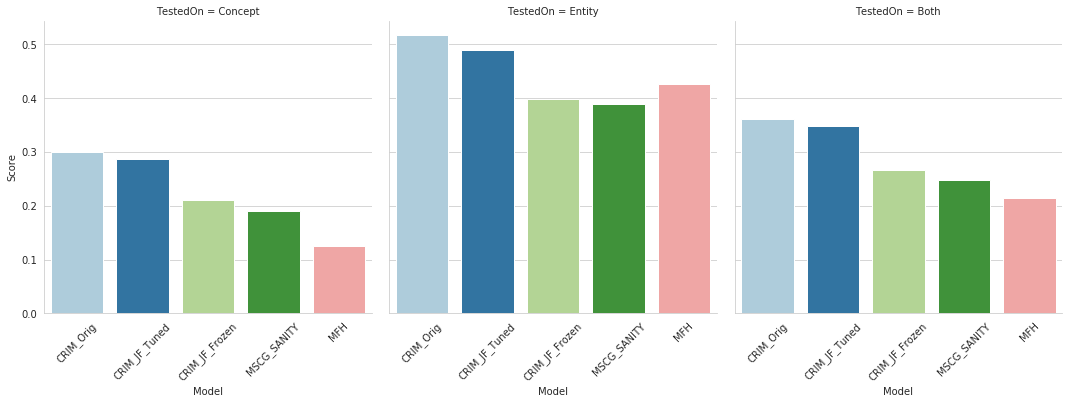
\includegraphics[width=0.8\textwidth]{images/jf_official_mrr.png} }\qquad
    \subbottom[MAP]{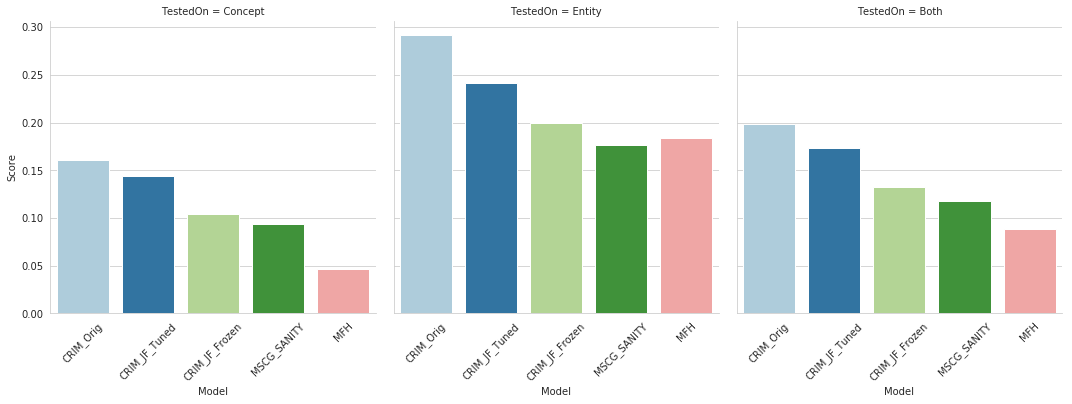
\includegraphics[width=0.8\textwidth]{images/jf_official_map.png} }%
    \caption{Comparison of best \ac{MRR} and \ac{MAP} scores with Shared Task top submissions, MFH baseline.}        
    \label{fig:jf_official_results}
\end{figure}
This sharp decline in performance should not be appraised in isolation, but in the context of the Shared Tasks submissions and baselines.  We show our best result in terms of \ac{MRR} and \ac{MAP}, alongside selected submissions' scores and the \ac{MFH} baseline in Figure~\ref{fig:jf_official_results}.  \textit{CRIM\_Orig} represents the original CRIM submission, which ranked first among all submissions in the English general-purpose subtask.  \textit{MSCG\_SANITY} was the second-best submission after CRIM, conspicuous for being the only submission to make use of an external resource, MS Concept Graph\footnote{originally known as Probase, which we briefly discussed in \cref{sec:lit_probase}.}.  Unfortunately, we do not know how the resource was used since the participants did not publish a technical paper to accompany their solution.  \ac{MFH} is a null model which emits the most frequent hypernyms in each word-type category.  \textit{CRIM\_JF\_Frozen} is the best model we achieved by learning the projection matrices while keeping the fastText embeddings frozen.  We resumed training \textit{CRIM\_JF\_Frozen}, this time tuning the embeddings but keeping the already-learned projections frozen.  We refer to the tuned model as \textit{CRIM\_JF\_Tuned}. 

Using the original fastText embeddings, our model surpasses \textit{MSCG\_SANITY}, enriched with external resources, in all word-categories.  The \ac{MFH} model scores the second highest \ac{MRR} when tested on entities.  This is because the 15 most frequent hypernyms, which only constitute  2\% of unique hypernyms in the entity test set, account for 22\% of all (entity) test word-pairs.  Contrast this with concepts term,  whereby the 15 most frequent hypernyms only account for 8.7\% of concept test word-pairs.  \ac{MFH} duly struggled with generating hypernyms for concept query terms.

After tuning the embeddings, the score margin between our model and the rest widened, but we were still not able to reach \textit{CRIM\_Orig}.  \citeauthor{bernier2018crim} conducted a series of ablation tests, each time setting a key hyperparameter to the default value or disabling it entirely.  Their \ac{MRR} ranged from 17.15 to 35.46; \ac{MAP} ranged from 8.01 to 19.47.  The main contributors to good performance were: multiple projections (they used 24, we used 10); 10 negative examples (we also opted for 10); initialising the projections by adding random noise to an identity matrix (we multiplied random noise to an identity matrix); tuning the embeddings.  Embeddings tuning was the most crucial decision of all; with frozen word2vec embeddings their model managed 0.172 \ac{MRR} and 0.080 \ac{MAP}.  \textit{CRIM\_JF\_Frozen}, which we trained on frozen fastText embeddings (concepts+entities) for less than 15 epochs scored 0.267 \ac{MRR} an 0.133 \ac{MAP}.  Our results are a reasonable improvement on the original, which we attribute primarily to our choice of embeddings, and secondly to our shorter training cycle using the default learning rate (0.001).

\citeauthor{bernier2018crim} did not list all the model hyperparameters in their paper, but they included a configuration file\footnote{\url{https://github.com/gbcolborne/hypernym_discovery/blob/master/hparams.conf}}  to the published code on GitHub.  Parameter values which were specifically cited in the paper matched the values in the configuration file, an indication that they were not arbitrary.  This file indicated that the original CRIM model was trained for at least 200 epochs (based on the patience setting), the learning rate was set to 0.0002 and the gradient value clipped to 0.0004.  We speculate that this configuration caused the model to converge very slowly, which was necessary considering that embeddings were being tuned when the model had not yet acquired any knowledge of the task and large gradient updates would have disrupted the pretrained embeddings' knowledge.

In the end, our tuned model managed 0.348 \ac{MRR} and 0.173 \ac{MAP} when evaluating a mix of concept and entity test terms; the original CRIM scored 0.361 and 0.198 but at the cost of a considerably longer training time.

\subsection{Embeddings Tuning}
Tuning the embeddings for one or two epochs boosted the scores substantially.  We examined the generated hypernyms after embeddings tuning to appraise the qualitative improvements in the model's performance.  In Table~\ref{tab:ft_tuned_predictions}, we illustrate a sample of high-quality predictions made by the tuned model.  The predicted words in bold matched the gold-standard.
\begin{table*}\centering
    \begin{tabular}{@{}lcl@{}} \toprule
    \textit{Word} & \phantom{a} & \multicolumn{1}{c}{\textit{Top 5 Predictions}} \\ \midrule
    azathioprine && \textbf{medicine}, \textbf{pharmaceutical\_drug}, \textbf{drug}, disease, medical\\
    blazonry && \textbf{picture}, illustration, work\_of\_art, \textbf{emblem}, \textbf{figure}\\
    flood && \textbf{natural\_phenomenon}, \textbf{physical\_phenomenon}\\
    && atmospheric\_condition, weather\_condition, \textbf{phenomenon},\\
    hardpan && \textbf{soil}, plant, soil\_structure, dirt, sand\\
    hostile\_fire && \textbf{war}, \textbf{military\_operation}, \textbf{military\_action},\\ 
    && military, military\_force\\
    postdoc && \textbf{person}, \textbf{scholar}, \textbf{researcher}, faculty\_member, leader\\
    president\_lyndon\_johnson && \textbf{person}, \textbf{leader}, \textbf{politician}, \textbf{political\_leader}, legislator\\
    slovenia && \textbf{country}, \textbf{state}, city, municipal\_government, territory\\    
    \bottomrule
    \end{tabular}
    \caption{Examples of accurate predictions after tuning fastText embeddings.}\label{tab:ft_tuned_predictions}
\end{table*}

However, a closer inspection of the results uncovered a detrimental side-effect: the model tended to suggest frequently occurring, but entirely unrelated, hypernyms as likely candidates for test words.  We chose the concept and entity query terms for which no correct hypernyms were discovered before and after our fastText embeddings tuning.  In each case, we found the candidate words the model suggested with highest confidence and plotted their frequency in a histogram which can seen in Figure~\ref{fig:confident_bad_prediction_before_after_tuning}.
\begin{figure}[!ht]
    \centering
    \subbottom[Before tuning]{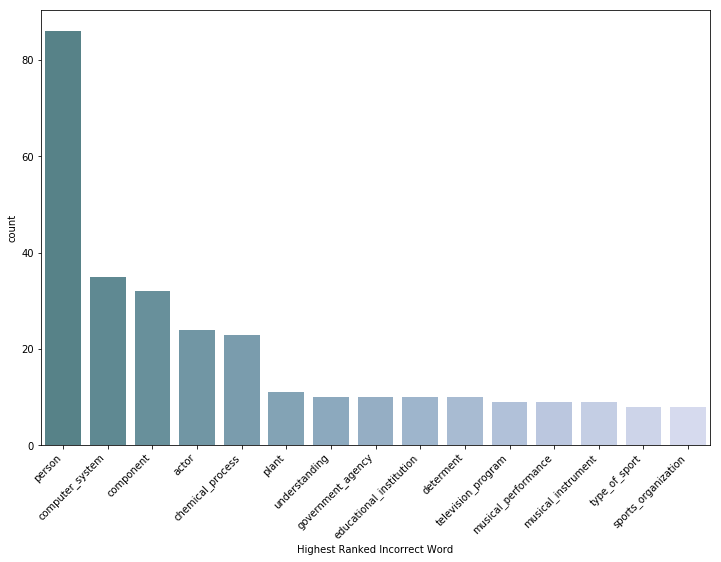
\includegraphics[width=0.6\textwidth]{images/ft_frozen_sum_highest_Ranked_incorrect.png} }\qquad
    \subbottom[After tuning]{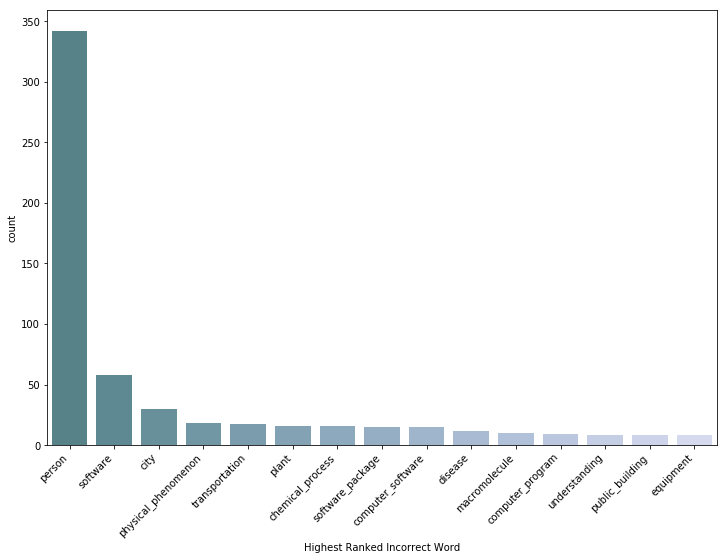
\includegraphics[width=0.6\textwidth]{images/ft_transfer_max_highest_Ranked_incorrect.png} }%
    \caption{Incorrect first-choice candidates before and after fastText embeddings tuning. }    
    \label{fig:confident_bad_prediction_before_after_tuning}
\end{figure}
In the top chart, \textit{person} was the most popular, first-choice incorrect term by the model trained on frozen embeddings but was only suggested for around 85 words.  After tuning, the model predicted \textit{person} as the most-likely hypernym for around 420 words.  Our relatively small dataset, coupled with the (relative) high concentration of terms related to the \textit{person} superordinate compelled the model to push the \textit{person} vector close to several projected hypernyms.  We did not have the opportunity to study the effect of the original, tuned embeddings, which the authors trained alongside the projection matrices.  It would have been interesting to see whether the same effect was observable or whether our result was due to our two-phase training strategy.
    %%%\textbf{This section should have a summary of the whole project.  The original aims and objective and whether these have been met should be discussed. It should include a section with a critique and a list of limitations of your proposed solutions.  Future work should be described, and this should not be marginal or silly (e.g.\ add machine learning models).  It is always good to end on a positive note (i.e.\ `Final Remarks').}
\chapter{Conclusions}
In this dissertation we tackled hypernym discovery, a topic in computational semantics which focuses on algorithms which can suggest the hypernyms of given query words.  Hypernym discovery is an evolution of the hypernym identification binary task, in which a model is expected to detect whether two words are related by hypernymy.  Pattern-based and distributional semantic models have been proposed as solutions to either task.  We focused on \textit{projection learning}, a supervised distributional method which learns a transformation matrix that when combined with a hyponym's embeddings generates an estimate of its hypernym vector.  Although originally developed as an alternative hypernym identification solution, it was later found to be well-suited for hypernym discovery.  We were further motivated to explore these algorithms after a  projection-learning-based model, submitted by the Computer Research Institute of Montreal, achieved the highest rank in all English subtasks in the SemEval-2018 Task 9 challenge.

\section{Achieved Aims and Objectives}
We divided our empirical work in two sections.  We first reviewed four projection learning methods and found two overlooked gaps in the literature.  To our knowledge, there was no published comparative analysis of all four models using a common dataset and evaluation metrics, which made it impossible to determine whether one or more models had an edge over the others.  Secondly, word2vec features were exclusively used to train all four models when applied to English-language hypernym discovery tasks.

Inspired by \citet{shwartz2017siege} work with unsupervised methods, we devised an experimental setup against which to test the chosen four projection model variants.  

\begin{table*}\centering
\begin{tabular}{@{}llll@{}}\toprule
\textbf{Model} & \textbf{Loss Function} & \textbf{Hyperparameter} & \textbf{Values}\\ \midrule
\multirow{2}{*}{\citep{Fu2014}} & \multirow{2}{*}{\ac{MSE}} & Embeddings & w2v, GloVe, ft\\
&& Clusters & 1, 10, 25\\ \midrule
\multirow{3}{*}{\citep{ustalov2017negative}} & \multirow{3}{*}{\ac{MSE}} & Embeddings & w2v, GloVe, ft\\
&& Clusters & 1, 10, 25\\
&& Regularisation & Asym., Neigh.\\ \midrule
\citep{yamane2016distributional} & Log-loss & Embeddings & w2v, GloVe, ft\\ \midrule
\multirow{4}{*}{\shortstack[l]{(Bernier-Colborne, and\\Barrière, 2018)}} & \multirow{4}{*}{Log-loss} & Embeddings & w2v, GloVe, ft\\
&& Projections & 1, 5, 10\\
&& Negative Samples & 1, 5, 10\\
&& $\lambda$ & 0, 0.1, 1\\
\bottomrule
\end{tabular}
\caption{Summary of tested factors in comparative analysis.}\label{tab:conc_experiment_summary}
\end{table*}

We borrowed the English Combined Dataset from \citet{ustalov2017negative} consisting of four high-quality datasets and partitioned it into $k=5$ folds.  We cross-validated each model using \ac{MRR}, \ac{MAP} and P$@k$ metrics mandated by \citet{camacho2018semeval} in the Shared Task.  We tested several versions of every model, each initialised with a different set of hyperparameters, chosen based on their claimed effect on performance in the respective publications.  We treated the embeddings like another hyperparameter, fitting each model with features extracted from publicly available, pre-trained embeddings created using word2vec (skip-gram, negative sampling), GloVe and fastText.  Each experiment yielded a distribution of scores which allowed us to perform multi-factor statistical tests using the \ac{ANOVA} framework.  Our salient findings are summarised below:
\begin{enumerate}
    \item The choice of embeddings has a significant effect on both \ac{MSE} and log-loss models.  fastText was significantly better than GloVe and word2vec in almost all of the tested configurations;
    \item GloVe embeddings are statistically a poor choice for log-loss models;
    \item Contrary to \citet{ustalov2017negative} findings, regularisation did not have a significant effect on English hypernym discovery, irrespective of the embeddings and number of clusters learned.  We confirmed that the scores increased when using regularisation in a single-cluster, word2vec context, but the improvement was not significant;
    \item Learning several projections in the multi-projection model has a significantly positive effect but is dependent on choice of embeddings;
    \item Log-loss models are significantly superior to \ac{MSE} models, while no difference was detected between the joint Yamane model and multi-projection CRIM model.  However, CRIM converges and generates hypernym predictions faster than Yamane.
\end{enumerate}

The \ac{MSE} models were published on GitHub by \citeauthor{ustalov2017negative}, and we modified the code to fit our experimental requirements.  Following the technical papers, we built the log-loss (binary cross-entropy) neural models and the training algorithms from scratch using TensorFlow's \texttt{Keras} machine learning framework.  We extended CRIM by integrating both asymmetric and neighbour regularisation terms from \citet{ustalov2017negative} training the model on both random and semantically-related negative samples. 

To predict hypernymy, the binary cross-entropy models require the query word as well as candidate hypernym which results in testing every vocabulary word (consisting of around 200K words) against each query term and selecting the words returning the highest hypernymy probability.  To accelerate this process we extracted the weights from the models and customised the forward-pass using fast \texttt{numpy} operations, significantly reducing the time required to generate the test dataset's query predictions.  

By addressing the aforementioned gaps and developing two models from scratch, we were able to develop a deep understanding of the models, which was the initial aim of this dissertation.  We showed that the multi-projection model developed by \citet{bernier2018crim} was statistically superior to the \ac{MSE} models that preceded it and faster to train than the original dot-product based model which inspired it \citep{yamane2016distributional}.  

We applied the multi-projection (CRIM) model to our second set of experiments: the English, general-purpose subtask outlined in the Shared Task.  For this task we trained word2vec, fastText and GloVe 300-dimensional embeddings on the 3-billion-word \textit{UMBC} corpus.  With frozen fastText embeddings and using no external resources, our model achieved \textbf{0.267} \ac{MRR} and \textbf{0.133} \ac{MAP}, a substantial improvement on the original CRIM which managed \textbf{0.172} \ac{MRR} and \textbf{0.080} \ac{MAP} when trained on frozen word2vec embeddings.  We also underline that the model converged in under 15 epochs, requiring less than 5 minutes training time.  The model would have ranked third overall in the Shared Task's general-purpose English subtask leader-board, preceded only by the \ac{CRIM} group, who submitted two runs.

Furthermore, we applied two sophisticated machine-learning techniques to the vanilla model.  We implemented a multi-task setup which trained two separate classifiers for concepts and entities whilst sharing the same feature extractor.  Despite the additional complexity, this had a negligible effect on the score, actually reducing performance on fastText vectors by a slight margin when compared to the vanilla setup.  We also tuned the embeddings, adopting a different approach to \citeauthor{bernier2018crim}.  Instead of training embedding and projections in the same phase, we split training into two phases.  We froze embeddings and trained projections in the first phase and froze the projections and tuned the embeddings in the second phase.  With only an additional 2 epochs of training, the strategy boosted our fastText \ac{MRR} and \ac{MAP} metrics by 30.5\% to 0.348 and 0.173 respectively.  Despite the improvement, we were not able to beat the original CRIM top-ranked submission which scored 0.361 \ac{MRR} and 0.198 \ac{MAP}.  However, to train embeddings and projections in one phase, the authors had to reduce the learning rate by an order of magnitude, clip the gradients and subsequently train their model for hundreds of epochs which is more expensive than our approach.

\section{Critique and Limitations}
The performance of projection learning methods seem to largely influenced by the choice of dataset.  This can be seen from the sharp decline in performance when evaluating our models on the Shared Task's more diverse dataset.  The more we move away from strict taxonomic definitions, the harder recognising hypernymy becomes.  This was observed on the Combined Dataset where 31\% of the word-pairs were related to the natural world.  Although there were significant fluctuations, all models performed relatively well on this task.  However, they do not possess the sophistication to discern among similar hypernyms.  For instance, the transformation matrix will project the hypernym for the term \textit{cat} in the vicinity of the \textit{animal} hypernym vector. But the model would also retrieve false positive candidates like \textit{invertebrate}, which are related to \textit{animal} but unrelated to \textit{cat}.

Supervised models are only as good as their training datasets.  We should keep in mind that there is an element of subjectivity even in the way humans perceive hypernymy.  This was evident in the Shared Task dataset which contained noisy training tuples, although it not clear how susceptible the models were to these samples.  In both Combined and Shared Task datasets, there was an observable tendency to project terms close to high frequency hypernyms seen during training.  Conversely, rarer hypernyms were unlikely to be discovered.  In Chapter 5, we plotted the relationship between test hypernym occurrence frequency in the Combined Data training set and average precision score per term.  There is a positive correlation between the two variables so we cannot rule out lexical memorisation.  However, we do not think the phenomenon is as pronounced as in simple binary classifiers trained to identity hypernymy; the projection models are also capable of surprising us by correctly retrieving relative rare hypernyms pertaining to non-trivial terms.

We achieved our best results when we tuned the embeddings.  However, we dwell on whether this strategy was merely a short-cut to amplify the scores and wonder whether the model ability to "understand" hypernymy really benefited from this.  Although we cannot argue with higher scores, we also noticed an increased predisposition towards projected the most frequent hypernym in the set.  The most galling example is the hypernym \textit{person} which was incorrectly predicted as a first-choice hypernym for nearly 350 test terms after tuning, up from 85 terms before tuning.

In this dissertation, we largely ignored the challenges of homonymy and polysemy. In the shared dataset, the organisers simplified the problem for us by conflating word senses into a single lexicalisation.   The vector representation of a polysemous word will arguably be a reflection of the context of that word in the corpus.  Word embeddings rely on latent dimensions which are not directly interpretable so we do not know exactly which sense/s of the word have been captured by the embeddings.  Finding the closest words to a polysemous in the embeddings space by cosine similarity may give some indication of how the word was "distilled" by the embeddings.  For instance in our word2vec embeddings trained on the \textit{UMBC} shared task corpus, the 15 most similar words to \textit{shell} are all related to the command-line interface sense of the work.  The projection learning methods show some ability at capturing the hypernyms for one sense of the word or another, but not likely to capture all word senses.  Specialised embeddings like \textsc{SenseEmbed} \citep{iacobacci2015sensembed} learn word embeddings for BabelNet \citep{navigli2012babelnet} synsets but require the corpus to be fully sense-disambiguated first.

Finally, projection learning systems have been used to discover hypernyms in languages other than English.  We reviewed work which describes their deployment on Chinese, Russian and Japanese.  However, we do not know how our favoured multi-projection model reacts to languages other than English.  

\section{Future Work}
Supervised methods generally benefit from larger training sets.  One way of augmenting the dataset is by using external lexical resources such as BabelNet.  BabelNet exposes a REST API which would allow us to search for a query term's co-hyponyms.  By definition co-hyponyms share the same hypernyms which we already have in our dataset.  We could then create new training examples by linking the co-hyponyms we retrieve from Babelet and the corresponding hypernyms from our given dataset.  Having a larger dataset would allow us to downsample highly frequent hypernyms in the dataset, much like embeddings training algorithm allow the subsampling of high frequency, less informative words.  Both dataset augmentation and subsampling were used in \cite{bernier2018crim} with mixed results.

Projection learning techniques depend on embeddings for word features.  However, the objective functions of the embeddings algorithms we chose are not designed with the hypernymy semantic relationship in mind.  In fact a term's most similar words in the word2vec, GloVe and fastText spaces tend to be synonyms or co-hyponyms.  Specialised embeddings which specifically learn the hypernym semantic relations have been developed.  \textit{HyperVec} is one example whereby the authors propose two objective functions to: train hypernym embeddings to have a higher Euclidean norm than hyponyms; to instil asymmetry in the embeddings such that the cosine similarity metrics is sensitive to word order \citep{nguyen2017hierarchical}.  \textit{HyperVec} embeddings can be used in an unsupervised context but whether they can be effectively used to train a projection learning model remains to be seen.

Arguably, one of the greatest challenges in hypernym discovery is the application of the techniques in a multi-lingual setting, especially for low-resource languages such as Maltese.  Applying effectively a projection learning approach would require high-quality embeddings which in turn depend on a corpus, large and diverse enough to somewhat encapsulate this relationship in a distributional manner.  Furthermore, a sufficiently large gold-standard dataaset would be required to train a projection learning model (or any other supervised model) as well as to evaluate the result.

The methodology employed by the SemEval 2018, Task 9 organisers which leveraged crowsdsourcing to verify semi-autonomously collected hypernyms works given a decent corpus and a rich, multilingual lexical resource such as BabelNet.  BabelNet already covers 2.5 million Maltese synsets and 5.1 millions word senses\footnote{Stats acquired from \url{https://babelnet.org/stats}} but we are not sure to what extent the synsets are linked semantically, especially considering that only 4,636 definition have been extracted from Maltese resources.  Possibly, a small evaluation Maltese gold-standard set can be created by translating an existing dataset such as the Combined Dataset we used in our own experiments.

In the absence of training data in a particular language, promising work has been done in the area of cross-lingual distributional semantics which leverage well-resourced languages to produce word representations for related, under-resourced languages.  In their recent paper, \citet{upadhyay2018robust} proposed an unsupervised method which learns bilingual, dependency-based word embeddings for a low-resource language by using a delexicalised parser trained on a treebank of a similar language.  There method was so far validated on a simulated low-resource language, whereby the resources were depleted manually.  Evaluating this method on a real under-resourced language like Maltese would be an interesting avenue of research to explore. 
    %%\appendix
    %%    \chapter{Media Content}

If the dissertation has a DVD or pendrive attached to it, you will need a section which explains what is on the media (structure, files, data, etc.).  This could be a table with filename and description.

\blindtext
     % these are just test names as I didn't know what you'd want
    %%    \chapter{Installation Instructions}
\blindtext
    
    %%    \chapter{User Manual}
\Blindtext
 

{\backmatter
    % Bibliography
    \if@openright\cleardoublepage\else\clearpage\fi
    \bibliographystyle{um-plainnat} %% specific plainnat does not show url for articles
    {\footnotesize\bibliography{chap1/introduction_biblio,chap2/background_and_lit_overview_biblio}}
	\printindex
}


\end{document}

%%% The End %%%